\documentclass[a4paper,11pt]{report}

\usepackage[T1]{fontenc}
\usepackage[utf8]{inputenc}
\usepackage[left = 2cm, top = 2cm, right = 2cm]{geometry}
\usepackage[autooneside=true, automark, headsepline, footsepline, plainfootsepline]{scrlayer-scrpage}
\usepackage{lmodern}
\usepackage{graphicx}
\usepackage{listings}
\usepackage[german]{babel}
\usepackage[font=small, margin=0pt ,labelfont=bf]{caption}
\usepackage[numbers,square]{natbib}
\bibliographystyle{alphadin}
\DeclareUnicodeCharacter{FEFF}{ }
\usepackage{tikz}
\usetikzlibrary{circuits.ee.IEC}
\usepackage{placeins}
\usepackage{pdfpages}
\usepackage{standalone}
\usepackage[hidelinks,plainpages=false,pdfpagelabels]{hyperref}
\usepackage{dirtree}
\usepackage[autostyle,german=quotes]{csquotes}

\ifoot*{\authormark}
\cfoot*{\pagemark}

\makeatletter
\newcommand*{\authormark}{}
\newcommand*{\markauthor}[1]{%
	\renewcommand{\authormark}{#1}%
}
\newcommand*{\chapterauthor}[1]{%
	\markauthor{#1}%
}
\makeatother

\usepackage{lipsum}

\begin{document}

\title{Projektdokumentation - MotorXP}

\author{Christian Brunner, Andreas Kölbl, \\
  Ricardo Krause, Bernd Krupinski, \\
  Andreas Lackner, Michael Schleinkofer, \\
  Franz Welker}

\automark{chapter}
\headheight1.3cm

\lehead{\headmark}
\lohead{\headmark}
\rehead{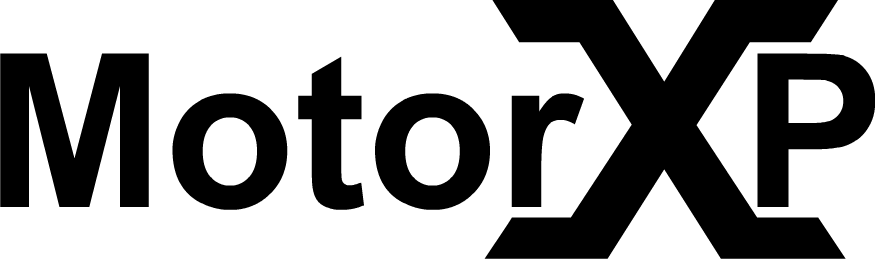
\includegraphics[height=25pt]{images/MotorXP}}
\rohead{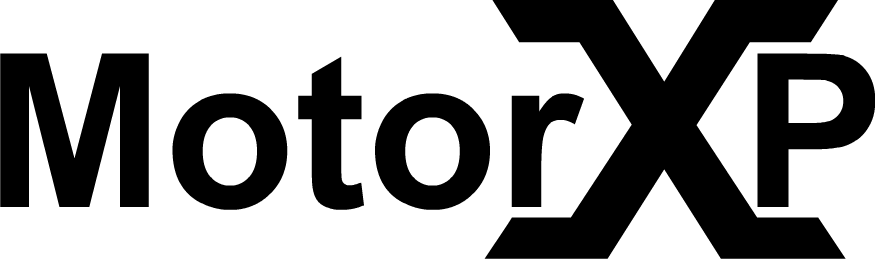
\includegraphics[height=25pt]{images/MotorXP}}


\renewcommand{\lstlistingname}{Code}
\lstset{
numbers=left,
stepnumber=1,
firstnumber=1,
numberfirstline=true,
breaklines=true}
\renewcommand{\figurename}{Bild}
\renewcommand{\refname}{Quellen}
\renewcommand{\bibname}{Quellen}
\renewcommand{\appendixname}{Anhang}
\renewcommand{\abstractname}{Zusammenfassung}
\renewcommand{\chaptername}{Kapitel}
\renewcommand\contentsname {Inhaltsverzeichnis}



\pagenumbering{Roman}
\makeatletter
\begin{titlepage}
  \centering
  \vspace*{0.02\textheight}
  
\includegraphics[width=\textwidth]{images/OTHLogo}\vspace*{0.1\textheight}
  {\huge\textbf{\\Projektdokumentation\\}}\vspace*{0.05\textheight}
  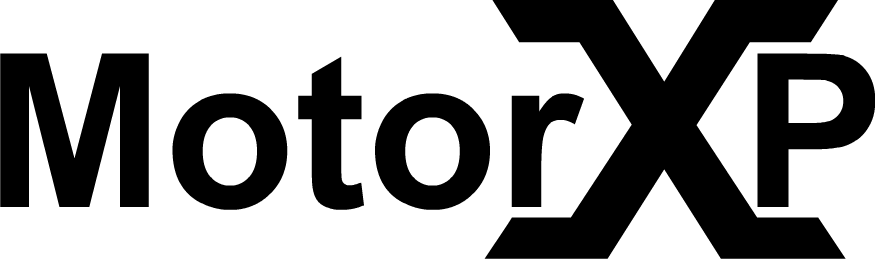
\includegraphics[height=2cm]{images/MotorXP}\vspace*{0.05\textheight}
  {\large\textit{\\Ansteuerung eines Brushless DC Motors mit einer grafischen Oberfläche und MATLAB Simulation}}\vspace*{0.03\textheight}
  {\\Vorlesung DT - Wintersemester 2016/17\\}\vspace*{0.2\textheight}
  {\@author}
\end{titlepage}
\makeatother
\tableofcontents


\begin{abstract}
Diese Dokumentation entstand im Rahmen der Vorlesung "Datenverarbeitung in der Technik" im Wintersemester 2016/17. 
In dem Projekt wurde ein mit einem BLDC-Motor bestückter Experimentierplatz angesteuert, Sensorwerte ausgelesen und eine bidirektionale Kommunikation zwischen $\mu$-Controller und einem PC wurde aufgebaut. Weiter wurde eine Benutzeroberfläche zur Visualisierung und Einstellung der Werte erstellt. Mit Hilfe einer Regelung wurden die eingestellten Werte auf dem Motor erreicht und gehalten. Parallel zu diesen Punkten wurde eine Simulation erstellt, welche den Motor in einem MatLab-Model nachempfindet und es wurden diverse Tests und Auswertungen angefertigt.
\end{abstract}
\pagenumbering{arabic}
\chapter{Projektstart}

Dieses Kapitel wurde von Herr Krause erstellt und betreut. Es beschreibt die Startphase des Projektes und zählt auf welche Tätigkeiten und Entscheidungen vor beginn des eigentlichen Projektes durchgeführt wurden. Es werden die Punkte Projektauftrag, Projektplan, Versionsverwaltung, Projektkommunikation und Dokumentenmanagement beschrieben.

\section{Projektauftrag}

Das Grundlegende Dokument für jedes Projekt ist der Projektauftrag, dieser Auftrag beinhaltet alle relevanten Parameter und Eckdaten des Projektes.

\begin{description}
\item[Projekttitel:] Der Arbeitstitel des Projektes.
\item[Projektnummer:] Eine in der Regel einzigartige Nummer zur Identifikation eines Projektes.
\item[Projektart:] Unterscheidung von verschiedenen möglichen Projekttypen.
\item[Projektleiter:] Bindeglied zwischen Kunden und Entwicklern mit überwachender und steuernder Tätigkeit.
\item[Projektauftraggeber:] Der Auftraggeber des Projektes.
\item[Projektkunden:] Können von Auftraggeber abweichen und auch mehrere sein.
\item[Projektdauer:] Legt den zeitlichen Rahmen des Projektes fest.
\item[Ausgangssituation/Problembeschreibung:] Dies beschreibt den aktuellen Zustand und das Problem, welches mit dem Projekt gelöst werden soll.
\item[Projektgesamtziel:] Zusammengefasste Beschreibung des Projektes mit dem zu erreichenden Ziel.
\item[Projektteilziele und -ergebnisse:] Detaillierte Auflistung der einzelnen Teilziele, mit messbaren zu erreichenden Ergebnissen.
\item[Nicht-Ziele / Nicht-Inhalte:] Abgrenzung des Projektes.
\item[Meilensteine:] Eckpunkte des Projektes mit ziel Datum, welche erreicht werden müssen um das Projekt erfolgreich zum Abschluss bringen zu können.
\item[Randbedingungen und -projektkontext:] Nebenbedingungen welche meist nicht direkt von Projektteam beeinflussbar, aber Notwendig zum erreichen des Projektzieles sind.
\item[Projektklassifizierung:] Parameter, welche das Projekt als Ziffer beschreiben und somit eine Vergleichbarkeit zwischen anderen Projekten schaffen.
\item[Projektorganisation:] Beinhaltet das Projektteam, weitere beteiligte Personen.
\item[Projektressourcen:] Alle für das Projekt zur Verfügung stehenden Ressourcen, beinhalten Personal und Material.
\item[Projektbudget:] Das zur Verfügung stehende Budget.
\item[Wirtschaftlicher oder sonstiger Nutzen:] Dieser Parameter ist meist wichtig für die Entscheider eines Projektes und soll den Gewinn durch das Projekt aufzeigen.
\item[Projektrisiken und -unsicherheiten:] Zeigt alle Risiken auf, welche zu einen Scheitern des Projekt führen könnten.
\item[Projektentscheidung:] Das Projekt muss vor beginn von einer Entscheidungsbefugten Person freigeben werden.
\item[Sonstige relevante Informationen:] Weitere wichtige Information.
\item[Anlagen:] Weitere Dokumente, welche das Projekt betreffen.
\end{description}

Der Projektantrag wurde von Herr Krause aufgesetzt, die Inhalte wurden gemeinsam erarbeitet und mit den Projektbeteiligten Personen abgestimmt. Der ausgearbeitete Antrag befindet sich im Anhang

\section{Projektplan}
Nach dem der Projektantrag erstellt wurde und die Ziele des Projektes bekannt waren, wurde ein detaillierter Projektplan erstellt. Dieser Plan wurde mit dem Open Source Tool \textit{OpenProj}\footnote{Link zum Projekt \url{http://www.serena.com/index.php/en/products/pod-update/}} erstellt und befindet sich ebenfalls im Anhang.\\
Der Projektplan beinhaltet alle erforderlichen Tätigkeiten und ermöglichte eine Abschätzung ob das Projekt mit den gegebenen Ressourcen in der gegeben Zeit durchführbar ist.

\section{Versionsverwaltung}
Als weiterer fundamentaler Pfeiler dieses Projektes wurde ein Versionsverwaltungssystem eingerichtet, welches dem Team ermöglichte ohne größere Probleme gemeinsam an dem Projekt zu arbeiten, ohne Gefahr zulaufen, die erstellten Artefakte\footnote{Arbeitsergebnis in einem Projekt} zu beschädigen.\\
Die Wahl viel auf das kostenlose und Open Source laufende Tool \textit{GIT}\footnote{Link zum Projekt \url{https://git-scm.com/}}, welches als verteiltes Versionsverwaltungssystem für die Software Komponenten und Dokumentation eingesetzt wird.\\
Das System GIT wurde gewählt, da es schon mehreren Mitglieder des Entwicklungsteams bekannt war und eine Vertiefung mit dem Umgang dieses Tools gewünscht wurde.\\
Durch den zusätzlichen Einsatz von \textit{Github}\footnote{Link zum Projekt\url{https://github.com/}}, welches ein Web-Interface für das eingesetzte GIT bietet, wurde es ebenfalls ermöglicht untereinander die Software Artefakte zu testen und direkt über Issues\footnote{engl. für Problem oder Angelegenheit}, Probleme und Änderungswünsche zu berichten.//
Die grobe Erstellung des Projektes auf Github übernahm der Herr Krause, die interne Struktur der einzelnen Arbeitspakete wurde von dem Herr Kölbl erledigt. 


\section{Kommunikation}
Für die Kommunikation der Projektgruppe wurde das ebenfalls Open Source laufende Tool \textit{Slack}\footnote{Link zum Projekt \url{https://slack.com/}} eingesetzt. Dieses Tool ermöglichte es gemeinsam und Themen orientiert zu kommunizieren und erleichterte durch Schnittstellen zur Versions- und Dokumentenverwaltung die erforderlichen Workflows.\\
Es wurde für jedes Arbeitspaket ein eigener Kommunikationsbereich eingerichtet und Mitglieder welche in einen bestimmten Bereich involviert oder interessiert waren, konnten diesen Bereichen beitreten und miteinander diskutieren.\\
Das Kommunikationstool wurde vom Herrn Krause eingerichtet.

\section{Dokumentenmanagement}
Im Team wurde entschieden, dass der Großteil der Dokumente für das Projekt nicht in die Versionsverwaltung gehört, deshalb wurde für die Verwaltung dieser Dokumente der Online Speicherdienst \textit{Dropbox}\footnote{Link zum Anbieter \url{https://www.dropbox.com/home}} gewählt. Dieses System wird bereits von den Studenten eingesetzt und bietet Schnittstellen zu aktuellen Textbearbeitungsprogrammen wie Microsoft Word und ebenfalls eine Integration zu Github und Slack ist möglich.\\
Es wurde eine grobe Ordnerstruktur\ref{fig:folderStruct} für die Dokumente festgelegt, welche sich an den Phasen des Projektes orientiert. Erstellte oder beschaffte Dokumente wurde in diese übersichtliche Struktur eingeordnet.\\
\begin{figure}[h]
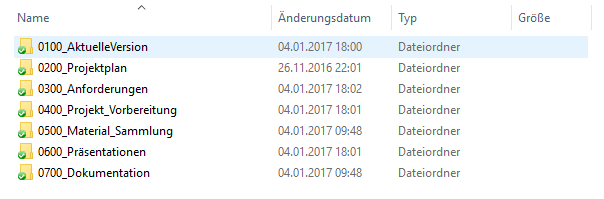
\includegraphics[scale=1]{projectdefinition/Bilder/FolderStructure}
\caption{Ordner Struktur Projekt}
\label{fig:folderStruct}
\end{figure}
Für Dokumente, welche gemeinsam bearbeitet wurden, erstellte man Templates. Diese konnten separat erstellt werden und wurden anschließend zusammengeführt. Dies ermöglichte einen einheitlichen Stil der Dokumente.

\graphicspath{{./communication/}}
\chapter{Arbeitspaket Kommunikation}
Für die Analyse, den Entwurf, die Impelementierung dieses Arbeitspaketes übernahm Herr Schleinkofer die Verantwortung. Während der Integration des Arbeitspaketes war Herr Schleinkofer unterstützend eingebunden.
\paragraph{}
Da die Projektspezifikation einen Datenaustausch zwischen $\mu$-Controller und PC enthält, muss diese auch im Projekt realisiert werden. Dabei kann sich auch am ISO/OSI-Schichtenmodell für Netzwerkkommunikation orientiert werden.
\section{Analysephase}
\subsection{Hardware}
Wie auch in der Physical-Layer behandelt, muss die Kommunikation in diesem Projekt zunächst physikalisch erfolgen. 
Dabei stellt sich die Frage, welche Möglichkeiten der Controller zur Datenübertragung an ein externes Gerät bietet. In dessen Handbuch ist aufgeführt, dass dort ein Universal Serial Interface Channel (USIC) Baustein zur Verfügung steht. Dies würde eine serielle Kommunikationsverbindung mit dem Universal Asynchronous Receiver Transmitter (UART) ermöglichen. Weitere Möglichkeiten sind auf dem Evaluation Board kaum gegeben. Dieses ist zwar für Ethernet vorbereitet, jedoch müssen dafür ein zusätzlicher Chip und eine RJ45-Buchse nachgerüstet werden. Eine selbst definierte und implementierte parallele Schnittstelle mit den GPIO-Ports wäre theoretisch auch möglich, jedoch in der Umsetzung zu komplex und zeitintensiv.
\paragraph{}
Die gemachten Überlegungen haben zur Folge, dass die Kommunikation zwischen Testplatz und PC über die serielle Schnittstelle abgewickelt wird. Nun muss entschieden werden, welches Gerät am Computer verwendet werden soll. Möglich wäre eine Kommunikation über ein serielles Kabel, welches an eine EIA-232 Schnittstelle des PC's angeschlossen wird. Dies ist jedoch mit einigen Problemen behaftet. Zunächst verfügen moderne Desktop Computer nur noch in wenigen Fällen über eine dedizierte EIA-232 Schnittstelle. Dies kann jedoch durch Verwendung eines USB-zu-Seriell-Adapters umgangen werden. Am $\mu$-Controller erfolgt dann der Anschluss an die GPIO-Pins. Allerdings muss dafür ein Adapter angefertigt werden, welcher auf der einen Seite einen D-Sub 9 Stecker und auf der anderen Seite mindestens die Pins 2 (Data Transceive), 3 (Data Receive) und 5 (Ground) als Stifte, passend zur Buchsenleiste des Evaulation Boards, weiterführt. Allerdings werden die Daten an der EIA-232 Schnittstelle mit bis zu 9 Volt übertragen. Dies stellt ein weiteres Problem dar, da an den Pins des Controllers nur 3,3 oder 5 Volt ausgegeben werden können. Auch kann ein Eingangssignal mit 9 Volt zu Schäden am $\mu$-Controller führen. Um dieses Problem zu umgehen, wäre es möglich, einen USB-zu-Seriell-Adapter mit integriertem Wandler-Chip zu verwenden.
\paragraph{}
Eine weitere Möglichkeit zur seriellen Kommunikation zeigt ein Beispielprojekt von Infineon für das Evaluation Board auf. In diesem erfolgt die Kommunikation zwischen PC und Controller über das USB-Kabel, welches am Debugging-Chip des Boards angeschlossen wird. Auch in diesem Projekt erfolgt der Datenaustausch mit Nutzung des USIC-Bausteins. Allerdings werden hier die Sende- und Empfangsleitungen an den ... Chip weitergeleitet. Für den PC ist darüber hinaus ein Windows-Treiber verfügbar, welcher einen "virtuellen Com-Port" zur Kommunikation mit dem Evaluation Board einrichtet und über den nun Daten im Rahmen des Beispielprojektes ausgetauscht werden können. Auf die Software des PC's hat diese Vorgehensweise keinen Einfluss, da ein virtueller Com-Port in der gleichen Weise verwendet wird, wie ein Hardware-Gerät. Ein weiterer Vorteil dieser Lösung ist, dass eine zusätzliche Stromversorgung des $\mu$-Controllers entfällt, da dies über das USB-Kabel der Kommunikation erfolgt.
\paragraph{}
Die Aufgaben der zweiten Schicht des ISO/OSI-Modells umfassen unter Anderem auch die Sicherung der Datenintegrität während der Übertragung. Dies geschieht im Fall des Ethernet-Protokolls mittels eines Cyclic Redundancy Check Verfahrens. Und auch andere Kommunikationsprotokolle nutzen diese Art der Integritätsprüfung um etwaigen Störungen während der Übertragung entgegenzuwirken.
\paragraph{}
Weitere Funktionen aus höheren Schichten des ISO/OSI-Modells scheinen in der gegebenen Zeit nicht umsetzbar oder werden schlichtweg nicht benötigt. Eine Adressierung der Kommunikationspartner ist in diesem Fall aufgrund der auf genau zwei beschränkten Anzahl an Teilnehmern genausowenig notwendig wie eine Sitzungsverwaltung ähnlich derer in OSI-Schicht 5. Eine Flusskontrolle oder Empfangsbestätigung ist im Falle zu übertragender Sensordaten auch nicht sinnvoll. Diese Sensordaten sollen nach den Anforderungen regelmäßig vom $\mu$-Controller an den PC gesendet werden. Bei höheren Drehgeschwindigkeiten des Motors würden diese nur unnötig Rechenzeit auf der Senderseite verbrauchen. Bei der Übertragung von Regelungsparametern allerdings könnte eine Empfangsbestätigung durch den $\mu$-Controller durchaus nützlich sein. Allerdings ist hierzu wie bereits erwähnt der Zeitrahmen zu eng gesteckt.
\subsection{Software}
Des weiteren muss noch Analysiert werden, wie die Sensor- und Regelungsdaten für die Kommunikation aufbereitet werden. Hierzu kommen verschiedene Serialisierungsverfahren in Betracht. Zunächst besteht die Möglichkeit die Daten als String zu formatieren und die einzelnen Zeichen als char-Daten seriell zu übertragen. Dies ist eine einfache Lösung, jedoch für zukünftige Änderungen nur schlecht erweiterbar. Es muss dazu für jeden Sensor die komplette Decodierungs-Routine des Strings auf beiden Kommunikationspartnern angepasst werden. Sollten nun in Zukunft beispielsweise mehr Experimentierplätze mit unterschiedlichen Sensoren existieren, muss darauf geachtet werden, dass zu jedem auch ein PC verwendet wird, dessen GUI auch den String mit den vorliegenden Sensorwerten auswerten kann.
\paragraph{}
Alternativ dazu kann ein Serialisierungsformat mit dem Namen "Protocol Buffers" (kurz: Protobuf)  verwendet werden. Dieses wurde durch die Firma Google entwickelt und ist für mehrere Programmiersprachen verfügbar. Dies ist wichtig, da die Software auf dem $\mu$-Controller in C, der Teil für den PC aber in C\# geschrieben wird. Der Vorteil dieser Lösung besteht darin, dass etwaige neu hinzukommende Sensoren einfach in die Protobuf-Nachrichten aufgenommen werden können. Kann eine Gegenstelle diesen Teil einer Nachricht nicht verarbeiten, so wird dieser einfach ignoriert.
\paragraph{}
\begin{lstlisting}[caption=Beispieldefinition einer Protocol Buffers Nachricht, label=lst:protoEx]
message Person {
  required string name = 1;
  required int32 id = 2;
  optional string email = 3;
}
\end{lstlisting}
Dies liegt in der Art, wie eine Nachricht in Protobuf aufgebaut ist. Zunächst wird diese in einer Beschreibungssprache definiert.
Im Code \ref{lst:protoEx} ist ersichtlich, dass eine "Message" aus mehreren Feldern und deren zugehörigen Identifiern ("= 1" für das Feld "name") besteht. Wird nun eine Nachricht um neue Felder erweitert, so kann ein Programm, welches jedoch noch die alte Beschreibung nutzt, eine neuartige Nachricht wieder deserialisieren. Die neuen Felder jedoch werden hierbei aufgrund des unbekannten Identifiers ignoriert. Protobuf verfügt darüber hinaus noch über einen Codegenerator. Das bedeutet: Der Entwickler definiert in der gezeigten Beschreibungssprache eine Nachricht. Anhand dieser Beschreibung wird nun duch den Generator zum Beispiel C\#-Code zur De-/Serialisierung erstellt. Zusätzlich wird dabei eine Datenstruktur definiert, die vom Entwickler im Programmcode mit den zu übertragenden Daten ausgefüllt werden und einfach in einen Bytestream verwandelt und wieder zurückverwandelt werden kann.
\paragraph{}
Zwar gibt es keine "offizielle" Implementierung von Protobuf für C, jedoch existiert ein Projekt mit dem Namen "nanopb" welches die grundlegenden Funktionen von Protocol Buffers in C speziell für Embedded Systems umsetzt.
\section{Entwurfsphase}
Der Ablauf der Kommunikation sollte relativ einfach gehalten werden, um in der vorgegebenen Zeit umsetzbar zu sein. Daher senden die Kommunikationspartner nur einfache Protobuf-Nachrichten. Der PC sendet Regelungsparameter und Ziel an den Controller. Dieser wiederum sendet regelmäßig die Daten der angeschlossenen Sensoren an die GUI auf dem PC. Um die Kommunikation für die angrenzenden Arbeitspakete so einfach wie möglich zu gestalten, soll die Schnittstelle nur aus wenigen Funktionen bzw. Methoden bestehen.
\subsection{Nachrichtendefinition}
Im System gibt es zwei Arten von Nachrichten. Die erste Art enthält die gesammelten Daten aller Sensoren auf dem Controller und wird von diesem an den PC verschickt. Die zweite Art enthält die Regelungsparameter und die Größe, welche geregelt werden soll. Diese Parameter können an der GUI eingestellt und an den $\mu$-Controller gesendet werden. Der grundlegende Aufbau beider Nachrichten auf Byte-Ebene ist gleich und wird in Bild \ref{fig:FrameOv} dargestellte. Den Beginn der Nachricht markiert ein Byte, welches die Anzahl aller Bytes der Nachricht (nachfolgend Frame genannt) enthält. Anschließend folgen die bereits von Protobuf serialiserten Daten als Reihe von Bytes. Den Abschluss des Frames bilden zwei Bytes, welche die CRC Prüfsumme enthalten. Bei der Prüfsumme handelt es sich um die 16-Bit große CRC-CCITT, welche unter anderem auch beim seriellen Datenübertragungsprotokoll HDLC verwendet wird. \cite[Absatz 1]{hdlcCrc}
\begin{figure}[h]
  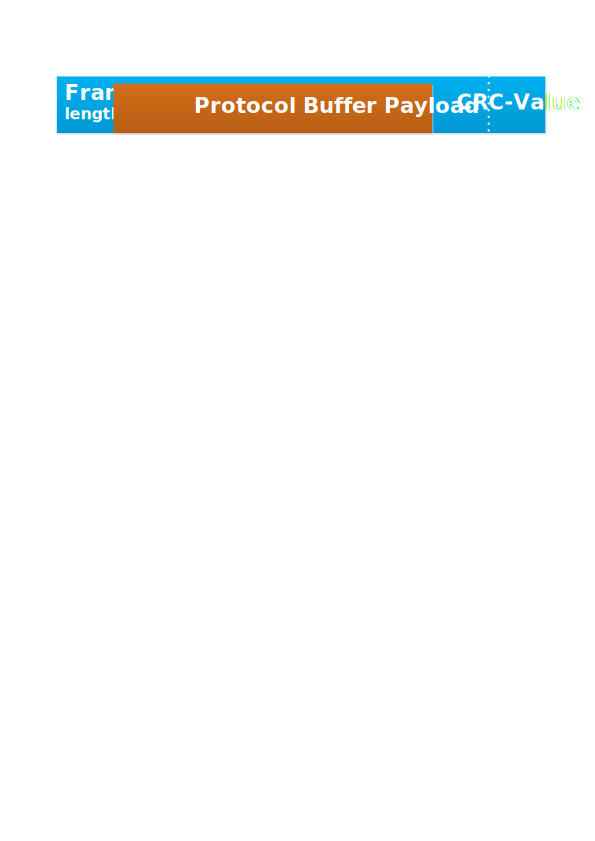
\includegraphics[width=\textwidth]{MessageFormat}
  \caption{Schematischer Aufbau eines Frames}
  \label{fig:FrameOv}
\end{figure}
\subsubsection{Sensordaten Nachricht}
Bei der Absprache mit den für die GUI verantwortlichen Entwicklern, kam folgende Anforderung hinzu: "Die Nachrichten sollen mit einem Zeitstempel oder einer fortlaufenden Nummer ausgestattet sein, um diese später unter Umständen nochmals sortieren zu können." Um auch für zukünftige Erweiterungen von Sensoren gerüstet zu sein, soll die Anzahl der Sensordaten in der Nachricht variabel gestaltet sein. Zudem wird jedem Sensorwert die ID des Sensors, welcher den Wert produzierte, zugeordnet. Um das alles zu erfüllen gilt für die Protobuf Nachricht folgende Beschreibung:
\begin{lstlisting}[caption=Beschreibung der Sensordaten Nachricht, label=lst:protoData]
//defining an entry of the data table
message DataEntry{
	uint32 SensorId = 1;
	double Data = 2;
}
//defining the real message
message SensorMsg{
	//Upcounting Nr
	uint64 SequenceNr = 1;
	//all Data
	repeated DataEntry DataTable = 2;
}
\end{lstlisting}
\subsubsection{Regelungsparameter Nachricht}
Das Team, welches die Regelung umgesetzt hat, stellt eine API bereit, welche neben den Parametern der P-, I- und D-Glieder eines Reglers auch die Regelgröße (z.B. Geschwindigkeit oder Drehmoment) und den Zielwert entgegennimmt. Dazu müssen diese Werte auch in der Protobuf Nachricht wie folgt berücksichtigt werden:
\begin{lstlisting}[caption=Beschreibung der Parameter Nachricht, label=lst:protoPara]
//defining the parameter message
message RegParams{
	uint32 target = 1;
	float paraP = 2;
	float paraI = 3;
	float paraD = 4;
	float tgtVal = 5;
}
\end{lstlisting}
Im Codebeispiel \ref{lst:protoPara} wird die Regelgröße mittels dem "target" Feld übermittelt. Dabei muss jedoch beachtet werden, dass bei beiden Kommunikationspartnern die Werte der gleichen Größe zugeordnet werden.
\subsection{Schnittstellendefinition}
\subsubsection{PC Bibliothek}
Für den Teil, welcher die Kommunikation auf Seiten der GUI übernimmt, soll eine Bibliothek auf C\#-Basis implementiert werden. Um nun Regelungsparameter an den Controller senden zu können, muss ein Datenobjekt beim Aufruf der Sende-Methode übergeben werden. Für den Empfang von Sensordaten ist es von Vorteil, das Hollywood-Prinzip anzuwenden. So soll die Bibiliothek nicht regelmäßig nach neuen Daten abgefragt werden. Vielmehr lößt deren API ein Event aus, welches die Verfügbarkeit neuer Werte anzeigt. Da sich bereits darauf festgelegt wurde, einen virtuellen Com-Port zur Kommunikation zu verwenden, soll dieser nun auch bei der Initialisierung der API als String oder gleich als ComPort-Objekt mit angegeben werden. 
\subsubsection{Controller Funktionen}
Ähnlich zur PC Bibliothek sollen die Funktionen auf dem $\mu$-Controller aufgebaut werden. Es soll zunächst eine Funktion zur Initialisierung der Kommmunikation bereitgestellt werden. Darüber hinaus soll es eine Funktion zum Setzen und eine weitere zum Versenden der gesammelten Sensordaten geben. Während der Analysephase wurde ersichtlich, dass auf dem Controller ein DMA-Baustein (Direct Memory Access) genutzt werden kann, um die Nachrichten-Bytes vom und zum UART-Modul zu übertragen. Dies erleichtert die Handhabung der Kommunikationsfunktionen dahingehend, dass nun beim erfolgreichen Empfang von Regelungsparametern ein globales Flag gesetzt werden kann, welches dies gegenüber der Regelungsschleife anzeigt. Eine weitere Aktion bezüglich des Datenempfangs von Seiten der Regelung ist somit nicht erforderlich. Die so empfangenen Regelungsparameter sollen nun nach Erhalt in global sichtbare Variablen abgelegt werden. Dies geschieht auf Wunsch des für die Regelung verantwortlichen Teams.
\section{Implementierung}
Da beide Endpunkte gänzlich unterschiedliche Eigenschaften und Ressourcen besitzen, gibt es zwei separate Softwareprojekte. Die Implementierung der Bibliothek erfolgt wie bereits erwähnt in C\# und unter Visual Studio 2013. Für die Implementierung des Kommunikationsmoduls auf dem Controller wird die Programmiersprache C unter DAVE 4 genutzt. 
\subsection{PC Bibliothek}
\begin{figure}
  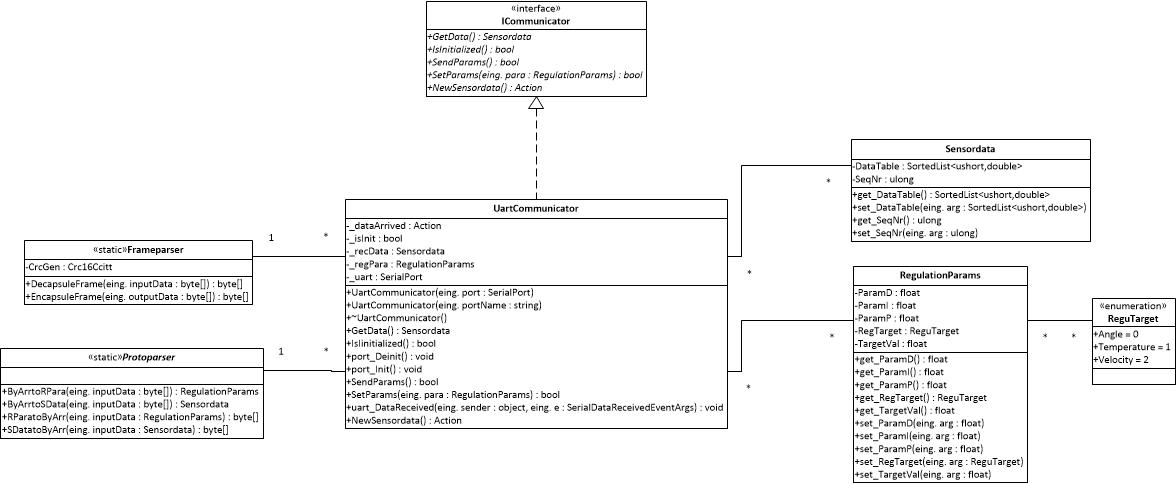
\includegraphics[width=\textwidth]{LibraryClasses}
  \caption{wesentliche Klassen der implementierten Bibliothek für die GUI}
  \label{fig:guiclasses}
\end{figure}
Wie aus Bild \ref{fig:guiclasses} ersichtlich ist, dient das Interface "ICommunicator" als API zur GUI hin und die Klasse UartCommunicator ist die Hauptklasse. Diese versammelt alle Funktionalität zum Senden und Empfangen von Nachrichten in sich. Bei der Erstellung eines Objektes dieser Klasse wird auch sofort die Initialisierungsmethode aufgerufen. In dieser wird das SerialPort-Objekt, welches zuvor dem Konstruktor angezeigt wurde, parametriert und geöffnet. Die gesetzten Parameter sind in den Zeilen 5 bis 12 im Anhang \ref{ComAPP:ComPortSettings} ersichtlich. Da zur Übertragung die USB-Schnittstelle mit nur zwei Signalleitungen genutzt wird, ist es nicht möglich für die Kommunikation einen Handshake auszuwählen bzw eine hardwaregesteuerte Flusskontrolle anzugeben. Dies wäre nur bei einer Verwendung der EIA-232 Schnittstelle möglich, da hier zusätzliche Leitungen für diese Zwecke existieren. Aus diesem Grund sind die Parameter "Handshake", "DtrEnable" und "RtsEnable" auf None bzw. false gesetzt. Alle weiteren Parameter wurden so gewählt, dass diese bereits bekannten Einstellungen für andere serielle Kommunikationen entsprechen.
\paragraph{}
Die Eigenschaft "ReceivedBytesThreshold" wurde auf 10 gesetzt. Dies bedeutet, dass nach 10 empfangenen Bytes die Methode aufgerufen wird, welche auf dem "DataReceived"-Ereignis des SerialPort-Objektes registriert wurde. Dies ist die private Methode des UartCommunicators. In dieser ist die Logik für den Empfang von Nachrichten implementiert.
\paragraph{}
Bei einem Empfang von Daten auf der seriellen Schnittstelle, wird zunächst das erste Byte im Eingangspuffer gelesen. Da dies die Framelänge darstellt (vgl. Bild \ref{fig:FrameOv}), kann nun daraus geschlossen werden, wie lang die empfangene Nachricht tatsächlich ist. Anschließend wird die nun bekannte Anzahl an Bytes in den Bearbeitungspuffer gelesen. Auf diesem Bearbeitungspuffer wird nun zunächst der Frame mit der statischen Methode "DecapsuleFrame" entpackt und folgend die Protobuf-Nachricht in ein Sensordata-Objekt umgewandelt. Am Ende der Empfangsprozedur wird das Event NewSensordata ausgelöst, welche anzeigt, dass neue Sensordaten vom UartCommunicator-Objekt abgeholt werden können. Dies geschieht mit der GetData-Methode.
\paragraph{}
Um nun Regelungsparameter versenden zu können, muss die GUI dem UartCommunicator-Objekt zunächst mit der SetParams-Methode ein Datenobjekt übergeben. Dieses Datenobjekt der Klasse RegulationParams kann nun mit der Methode "SendParams" an den Controller gesendet werden. Hier ist der Ablauf in umgekehrter Reihenfolge zu durchlaufen. Das Datenobjekt wird nun von einer statischen Methode in eine Protobuf-Nachricht serialisiert und in einen Bearbeitungspuffer abgelegt. Dieser Bearbeitungspuffer wird im Anschluss mit einem Frame-Header und einem Frame-Tail ausgestattet. Abschließend wird der Bearbeitungspuffer versendet. In Zeile 9 im Anhang \ref{ComAPP:SendWait} ist zu erkennen, dass nach jedem gesendeten Byte des Bearbeitungspuffers 30 Millisikunden gewartet wird. Dies ist notwendig, da ein kontinuierliches Senden der Datenbytes den DMA-Baustein auf dem Microcontroller überlastet und dort nur noch unverwertbare Daten vorhanden wären.
\paragraph{}
Für die Umwandlung der Daten in Protobuf-Nachrichten und umgekehrt, existiert eine separate Protoparser-Klasse. Diese stellt wie im Klassendiagramm ersichtlich statische Methoden zur Verfügung. Um aus einem Bytearray mit Protobuf-Daten ein Sensordaten-Objekt zu erzeugen, nutzt die Methode "ByArrtoSData" zunächst ein SensorMsg-Objekt aus dem durch Protobuf generierten Code. So wird ein Protobuf-Objekt erzeugt, aus welchem im Anschluss die Daten für das Sensordaten-Objekt extrahiert werden.
\paragraph{}
In die "Gegenrichtung" muss in umgekehrter Reihenfolge vorgegangen werden. Zunächst wird ein Objekt aus dem von Protobuf generierten Code mit den Daten eines Sensordata-Objektes gefüllt. Dieses Protobuf-Objekt wird nun mit der Methode "ToByteArray" in ein Array aus 8-Bit-Zahlen umgewandelt, welches wieder zurückgegeben wird. Die gleiche Vorgehensweise gilt auch für die Methoden "RParatoByArr" bzw. "ByArrtoRPara" welche die Regelungsparameter in eine Protobuf-Nachricht um- bzw. zurückwandeln.
\paragraph{}
Für die Handhabung der Nachrichten-Frames stehen in der Klasse "Frameparser" zwei statische Methoden zur Verfügung. Die Methode "DecapsuleFrame" nimmt zunächst das übergebene Byte-Array mit dem Frame und berechnet ab Element 2 die CRC-Summe. Da am Ende des Frames bereits ein 16 Bit CRC-Wert steht, entspricht das Ergebnis der aktuellen CRC-Erzeugung bei einem korrekten Frame 0. Ist dies der Fall, so werden die Bytes der Payload in einem neuen Byte-Array zurückgegeben.
\paragraph{}
Um nun ein Byte-Array mit einer Protobuf-Nachricht mit einem Frame auszustatten, existiert die statische Methode "EncapsuleFrame". Über das übergebene Array wird in dieser Methode die 16 Bit lange CRC-Summe berechnet. In ein neues Byte-Array wird nun an erster Stelle die Länge des alten Arrays + 3 als neue Framelänge abgelegt. Im Anschluss an das erste Element folgt nun das bereits übergebene Array. Abschließend werden beide Bytes des CRC-Wertes in das neue Array eingefügt, bevor dieses wieder zurückgegeben wird.
\paragraph{}
Für die Berechnung der CRC-CCITT in C\# wurde eine Klasse verwendet, welche unter sanity-free.org \cite{crc} zur Verfügung steht. Als Initialwert bei der Instanzierung wurde "NonZero1" verwendet. Es ist darauf zu achten, dass dieser Wert mit dem Initialwert auf dem $\mu$-Controller übereinstimmen muss.
\subsection{Controller Funktionen}
Die Implementierung des Kommunikationsmoduls auf dem $\mu$-Controller erfolgte unter Verwendung des Programmes DAVE 4 von Infineon. Bild \ref{fig:xmcobj}Damit ist es relativ einfach, die auf dem Chip vorhandenen Ressourcen zu parametrieren und zu nutzen. Im Rahmen der Kommunikation werden hauptsächlich zwei sogenannte Apps verwendet. Eine davon dient zur Parametrierung des UART-Bausteins, die andere zur Parametrierung der CRC-Erstellung.
\begin{figure}
  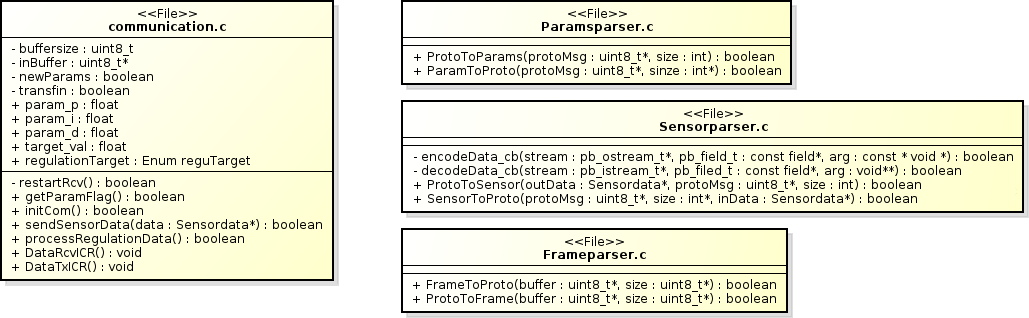
\includegraphics[width=\textwidth]{XMCObjects}
  \caption{Implementiertie Funktionen des Kommunikationsmoduls auf dem $\mu$-Controller}
  \label{fig:xmcobj}
\end{figure}
\paragraph{}
Als Hauptobjekt der API dient die Datei communication.c. Hier wird zunächst die Funktion \\"initCom" zur Verfügung gestellt. Damit werden die globalen Variablen zur Übergabe der Regelungsparameter auf einen definierten Anfangszustand gebracht und der Empfang von Nachrichten auf dem UART-Baustein angestoßen. Dazu wird die Funktion "UART\_Receive" genutzt, welche vom Programm DAVE bei Verwendung der UART-App automatisch generiert werden kann. Allerdings wird hier nur ein Byte gelesen. Denn nach der Definition des Frameaufbaus, resultiert daraus die Framelänge. Ist dieses Byte erfolgreich gelesen worden, so wird die Callback-Funktion "DataRcvICR" durch einen Interrupt aufgerufen.
\paragraph{}
In dieser Callback-Funktion wird nun ein Bearbeitungspuffer passend für den Empfangenen Frame erstellt und in diesem die noch fehlenden Bytes eines nach dem anderen abgelegt. Wurde nun der gesamte Frame erfolgreich empfangen, so wird ein Flag gesetzt. Falls nicht, wird die Kommunikation neu initialisiert.
\paragraph{}
Darüber hinaus existiert eine Funktion, welche bei ihrem Aufruf das Flag aus der Callback-Funktion zurückgibt und so anzeigt, ob eine neue Nachricht mit Regelungsparametern vorliegt. Wird hier true zurückgegeben, kann die Regelung die Funktion "processRegulationData" aufrufen. Damit wird die Verarbeitung der empfangenen Datenbytes und das erneute Empfangen von Nachrichten angestoßen.
\paragraph{}
Um nun die Daten der Sensoren zu versenden, kann die Funktion "sendSensorData" genutzt werden. Dieser muss ein Pointer auf eine Struktur des Typs "Sensordata" mit übergeben werden. Diese Funktion nun wandelt die übergebenen Daten zunächst in eine Protobuf-Nachricht und dann in einen Frame um. Dann wird dieser Frame mit der von DAVE generierten Funktion "UART\_Transmit" übertragen. Da in der Entwurfsphase beschlossen wurde, dass die Übertragung der Daten vom und zum UART-Baustein mittels DMA geschieht, gibt es für den Interrupt eines erfolgreichen Versendens der Daten eine Callback-Funktion. In dieser Funktion wird ein statisches Flag gesetzt, welches verhindert, dass der DMA-Baustein erneut Daten senden muss, obwohl die "alte" Nachricht noch nicht komplett versendet worden ist.
\paragraph{}
Für die Umwandlung der Sensordaten in eine Protobuf-Message, steht die Funktion "SensorToProto" in der Datei Sensorparser.c zur Verfügung. In dieser wird zunächst eine von nanopb generierte Struktur soweit wie möglich ausgefüllt. Um jedoch das wiederholte Feld für die sogenannte "DataTable" auszufüllen, muss eine Callback-Funktion definiert werden. Dies ist die in der gleichen Datei befindliche "encodeData\_cb". Mit dem Aufruf der ebenfalls durch nanopb generierte Funktion "pb\_encode" wird nun die Message-Struktur in ein Byte-Array umgewandelt.
\paragraph{}
In der Callback-Funktion muss für jeden Eintrag in der "DataTable" aus der Protobuf-Message die funktion "pb\_encode\_submessage" aufgerufen werden. Funktionen zum decodieren der Sensordaten-Nachricht wurden in der gleichen Datei implementiert, werden hier jedoch nicht weiter ausgeführt, da diese im Rahmen des Projektes nicht genutzt werden.
\paragraph{}
Um nun empfangene Nachrichten mit Regelungsparametern dekodieren zu können, wird die in der Datei Paramsparser.c implementierte Funktion "ProtoToParams" genutzt. Aufgrund des einfacheren Aufbaus der Parameter-Message, müssen hier nach dem Aufruf der generierten Funktion "pb\_decode" nur die Parameterwerte aus einer temporären Struktur in die zuvor genannten, globalen Variablen übertragen werden. Auch in dieser Datei existiert wieder eine Funktion, welche Regelungsparameter in eine Protobuf-Nachricht umwandelt. Auch diese wurde nur der Vollständigkeit wegen implementiert und wird im Projekt nicht genutzt.
\paragraph{}
Zum Ein- und Entpacken der Messages in Frames, können die Funktionen "ProtoToFrame" bzw. "FrameToProto" aus der Datei Frameparser.c genutzt werden. Bei der Erstellung des Frames wird der übergebene Puffer auf die richtige Größe gebracht. Weiter werden am Anfang die Anzahl der Bytes des gesamten Frames und am Ende zwei Bytes mit dem CRC-Wert abgelegt. Um diesen Wert zu erhalten werden die durch DAVE generierten Funktionen "CRC\_SW\_CalculateCRC" sowie "CRC\_SW\_GetCRCResult" genutzt. Bei der Nutzung der Funktion "ProtoToFrame" ist darauf zu achten, dass das erste Element des übergebenen Puffers keine Daten der Payload enthält, da hier die Framelänge abgelegt wird.
\paragraph{}
In der Funktion "FrameToProto" werden auch die genannten Funktionen zur Generierung des CRC-Wertes genutzt. Hier wird jedoch das Ergebnis auf 0 überprüft. Wie bereits geschildert, bedeutet beim Entkapseln des Frames ein CRC-Wert gleich 0, dass kein Fehler während der Übertragung aufgetreten ist. Ist dies der Fall, so wird der Bearbeitungspuffer um 2 Elemente verkleinert. Das dritte nun überschüssige Byte des Puffers wird nicht gelöscht, da ein dadurch notwendiges Verrücken der Payload im Puffer zu ressourcenintensiv ist. Allerdings wird die Größe der Payload durch die Funktion "FrameToProto" richtig zurückgegeben.
\paragraph{}
Außerdem existieren noch zwei Header-Dateien com\_types.h und SensorIDs.h. In der Ersteren befinden sich die Definitionen für die Sensordata-Struktur, welche die Regelung zur Übergabe der Sensorwerte nutzt, sowie der Aufzählung der möglichen Regelgröße. In der Letzteren wurden die ID's der einzelnen Sensoren für die Zuordnung der Werte abgelegt.
\paragraph{Parametrierung der DAVE Apps}
Hier werden alle in den DAVE Apps getroffenen Einstellungen aufgeführt. Die notwendigen Apps "UART [4.1.8]" und "CRC\_SW [4.0.6]" werden über den Menüpung "DAVE -> Add New APP …"... hinzugefügt.
\begin{figure}
  \begin{minipage}{0.4\textwidth}
    \centering
    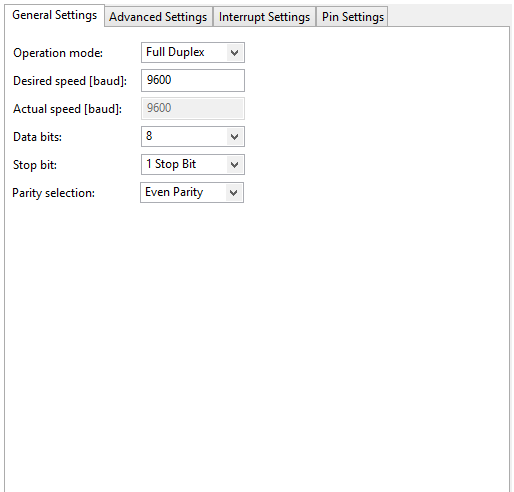
\includegraphics[width=\textwidth]{UARTgeneralSet}
    \caption{Grundlegende Einstellungen der UART-App: Diese müssen mit den Einstellungen der C\#-Bibliothek übereinstimmen.}
  \end{minipage}
  \begin{minipage}{0.4\textwidth}
    \centering
    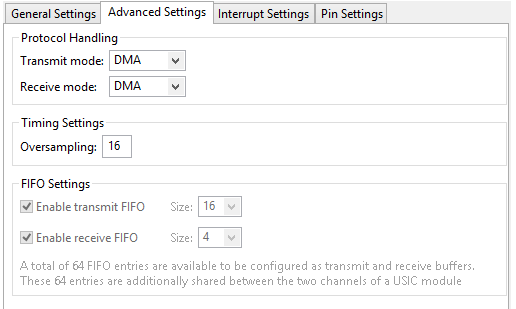
\includegraphics[width=\textwidth]{UARTadvancedSet}
    \caption{Weiterführende Einstellungen der UART-App: Beide Richtungen werden per DMA gehandhabt.}
  \end{minipage}
\end{figure}
\begin{figure}
  \begin{minipage}{0.4\textwidth}
    \centering
    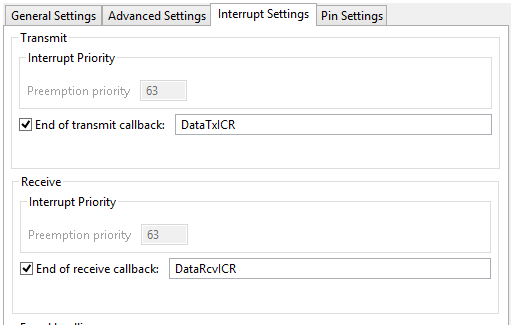
\includegraphics[width=\textwidth]{UARTinterSet}
    \caption{Interrupt Einstellungen der UART-App: Hier werden die Callback-Funktionen angegeben.}
  \end{minipage}
  \begin{minipage}{0.4\textwidth}
    \centering
    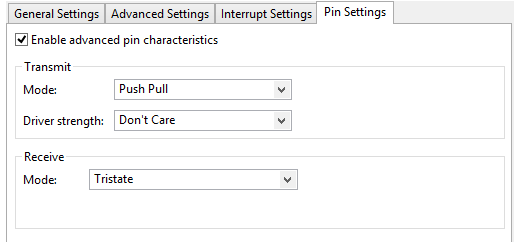
\includegraphics[width=\textwidth]{UARTpinSet}
    \caption{Einstellungen der GPIO-Pins für die UART-App}
  \end{minipage}
\end{figure}
\begin{figure}
  \begin{minipage}{0.4\textwidth}
    \centering
    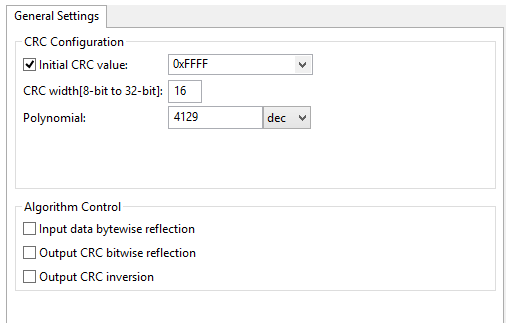
\includegraphics[width=\textwidth]{CRCgeneralSet}
    \caption{Einstellungen für die CRC-Berechnung: Auch hier müssen die Einstellungen mit denen der C\#-Bibliothek übereinstimmen}
  \end{minipage}
  \begin{minipage}{0.4\textwidth}
    \centering
    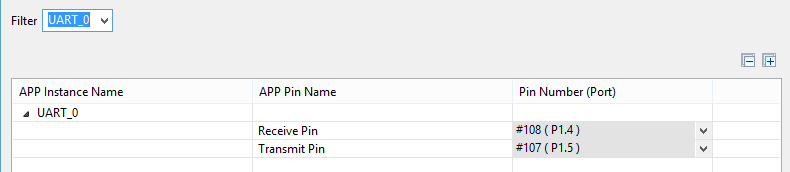
\includegraphics[width=\textwidth]{PinAlloc}
    \caption{Zuordnung der GPIO-Pins unter "DAVE -> Manual Pin Allocator; Die Pins P1.4 und P1.5 sind mit dem Debug-Chip verbunden."}
  \end{minipage}
\end{figure}
\section{Integration}
\begin{figure}
  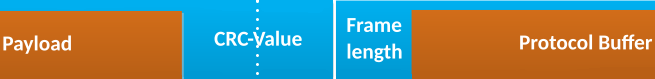
\includegraphics[width=\textwidth]{WorkBufferFail}
  \caption{Inhalt eines falsch interpretierten Bearbeitungspuffers}
  \label{fig:FrameFail}
\end{figure}
Die Integration der beiden Module in die Regelung erfolgte hauptsächlich durch Herrn Krupinski. Auf Seiten der GUI übernahm diese Aufgabe Herr Krause. Herr Schleinkofer war in beiden Fällen nur beratend tätig. Seine Hauptaufgabe während dieser Phase bestand in der Behebung der auftretenden Fehler. Bei einem ersten Zusammenfügen von Regelung und GUI wurde ersichtlich, dass das Senden der Nachrichten mit den Sensorwerten nur unzureichend robust war. Die Ursache bestand hauptsächlich im Design der Nachrichten und des Kommunikationsablaufs. Sind im Eingangspuffer des SerialPort-Objekts noch Rest-Daten, so interpretiert die Kommunikationsbibliothek diese fälschlicherweise als Beginn einer neuen Nachricht. Das erste Byte wird daher als Framelänge interpretiert. Ein neuer Frame wird dann nur unvollständig in den Bearbeitungspuffer übernommen (siehe Bild \ref{fig:FrameFail}). So befindet sich dort am Anfang die Hälfte der alten Nachricht und am Ende der Anfang der neuen. Dies führt zu einem Verwerfen des Inhalts im Bearbeitungspuffer. Dieses Verhalten wiederholt sich nun im weiteren Programmverlauf, sodass nun keine Sensordaten mehr empfangen werden können. Sender und Empfänger sind nicht mehr im "gleichen Takt". 
\paragraph{}
\begin{figure}
  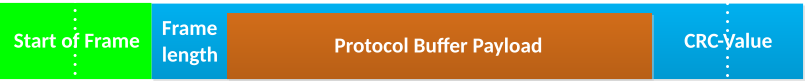
\includegraphics[width=\textwidth]{MessageFormat_enhanced}
  \caption{Verbessertes Nachrichtendesign mit Start of Frame}
  \label{fig:FrameEnhanced}
\end{figure}
Um dies zu verhindern, wird nun zu Beginn jedes Frames vom $\mu$-Controller ein 16 Bit langer Start of Frame Delimiter (kurz: SoF) mit übertragen (siehe Bild \ref{fig:FrameEnhanced}). Es ist bei der Wahl des SoF darauf zu achten, dass diese Bitreihenfolge möglichst einzigartig in der Kommunikation ist. Aus Bekanntheitsgründen und mangels Vergleichswerten aus der vorliegenden Kommunikation wurde dabei auf einen Teil des Musters eines Ethernet-Frames gewählt. Das erste Byte des SOF ist 0x55 und das zweite 0xD5. Es wären aber auch andere Werte denkbar. Die Bibliothek prüft nun vor dem Verarbeiten eines Frames, ob am Anfang des SerialPort-Eingangspuffers nun diese zwei Bytes vorhanden sind. Dies geschieht mittels eines einfach implementierten Zustandsautomaten. In einer Schleife wird nun immer das erste Byte des Eingangspuffers gelesen und verworfen. Folgendes Bild verdeutlicht den im Anhang \ref{ComAPP:SoFMachine} implementierten Automaten.
\begin{figure}
  \centering
  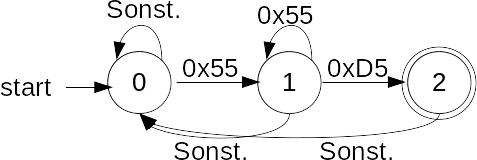
\includegraphics[width=0.4\textwidth]{Automat}
  \caption{Zustandsautomat zur erkennung des Start of Frame}
  \label{fig:Machine}
\end{figure}
\section{Ausblick}
Einige Funktionen für eine zuverlässige Kommunikation konnten aufgrund der beschränkten Zeit nicht mehr umgesetzt werden. So ist es von Vorteil, wenn auch die Nachrichten mit den Regelungsparametern einen Start of Frame vorangestellt bekommen. Dies würde wie auch auf der GUI-Seite verhindern, dass eine unvollständig empfangene Nachricht das Erkennen eines Framebeginns verhindert.
\paragraph{}
Darüber hinaus wäre noch vorstellbar, für die Übertragung der Regelungsparameter eine Empfangsbestätigung zu implementieren. Dies würde einem eventuell notwendigen mehrfachen Sendeversuch durch den Benutzer vorbeugen.
\paragraph{}
Weiterhin wurde bei einem Review des erstellten Codes ersichtlich, dass die DAVE-App zur Erzeugung des CRC-Wertes keinen Gebrauch der Flexible CRC Engine auf dem $\mu$-Controller macht. Aufgrund des Zeitdrucks war eine detailliertere Einarbeitung in die Parametrierung der Hardware nicht mehr möglich.


\chapterauthor{Andreas Lackner}

%todo einrückungen bei den Absätzen konsisten halten!
%todo Hurrenkind entfernen

\chapter{Arbeitspaket Sensorik}
Die Analyse, Implementierung und Integration, sowie der Aufbau der ben\"otigten Schaltungen f\"ur die Sensorik des Experimentierplatzes, war Aufgabe von Herrn Lackner mit Unterst\"utzung von Herrn Brunner f\"ur Hardware-relevante Problemstellungen.

\section{\"Uberblick}
Um den Betrieb des Motorexperimentierplatzes zu erm\"oglichen und sinnvolle Anwendungen zu finden, m\"ussen eine Reihe von relevanten Kenngr\"o{\ss}en, durch den Einsatz von Sensorik, gemessen und diversen Modulen, bzw. den Benutzern des Experimentierplatzes zur Verf\"ugung gestellt werden. \\
Die zu erfassenden Daten, die in der Analysephase des Projekts festgelegt wurden, ergeben sich haupts\"achlich aus den bereits verbauten und uns so zug\"anglichen Sensoren. Gemessen werden folgende Werte:
\begin{itemize}
\item \textbf{Drehwinkel} \\
Aktueller Winkel der Motorwelle, relativ zu einem Festgelegten Nullpunkt.
\item \textbf{Drehgeschwindigkeit} \\
Umdrehungen der Welle pro Zeiteinheit.
\item \textbf{Motor-Temperatur} \\
Temperatur des Motors, da dieser sich im Betrieb erhitzt.
\item \textbf{Hall Pattern} \\
Stellt eine alternative M\"oglichkeit da, den Drehwinkel zu ermitteln. Das Pattern wird haupts\"achlich zur Kommutierung eingesetzt, da sich daraus sowohl der passende Zeitpunkt als auch das korrekte Motor-Pattern ableiten lassen.
\end{itemize}
Für die Ermittlung definierten Werte stehen auf den Experimentierstand drei \textbf{Hall-Sensoren}, ein \textbf{Inkrementalgeber} und ein \textbf{Temperatursensor} zur Verfügung, die alle im Aufbau fest verbaut sind. 

\section{Entwicklungsumgebung}
Wie auch die anderen Module, die direkt mit dem aufgebauten Motor interagieren, befindet sich die gesamte Software für die Sensorik auf dem Steuerungsmikrocontroller. Diese Aufgabe erfüllt momentan ein \textbf{XMC4800} von Infineon, aufgebaut auf einem Relax Kit V1. Da die Interaktion mit den Sensoren Hardware-nahe Programmierung erfordert, ist sämtlicher Code in C geschrieben. Als IDE für die Entwicklung dient DAVE 4 von Infineon.

\subsection{DAVE 4}
DAVE ist eine von Infineon bereitgestellte Entwicklungsumgebung für das Firmeneigene Controller Portfolio. Die Installationsdatei kann nach Registrierung bei Infineon direkt heruntergeladen werden. Während des Installationsprozesses werden ebenfalls automatisch die benötigten Treiber für den Debug-Chip auf dem Entwicklungsboard mit installiert. \\

\subsubsection{Projekt anlegen} 
DAVE bietet Standardm\"a{\ss}ig mehrere verschiedene Projekttypen an, die eine unterschiedliche Menge von bereits fertigem Code mit sich bringen. Bei einem \textbf{Empty Project} wird nur die HAL Bibliothek und die f\"ur den Controller ben\"otigten Startup Dateien bereitgestellt. Das \textbf{Simple Main} Projekt erstellt zus\"atzlich noch eine main.c Datei, mit einer leeren Main-Funktion. Entscheidet man sich für ein \textbf{Easy Start} Projekt, erh\"alt man Beispielcode der exemplarisch eine AD Wandlung vornimmt und einige Ausg\"ange setzt.

\begin{figure}[ht]
\centering
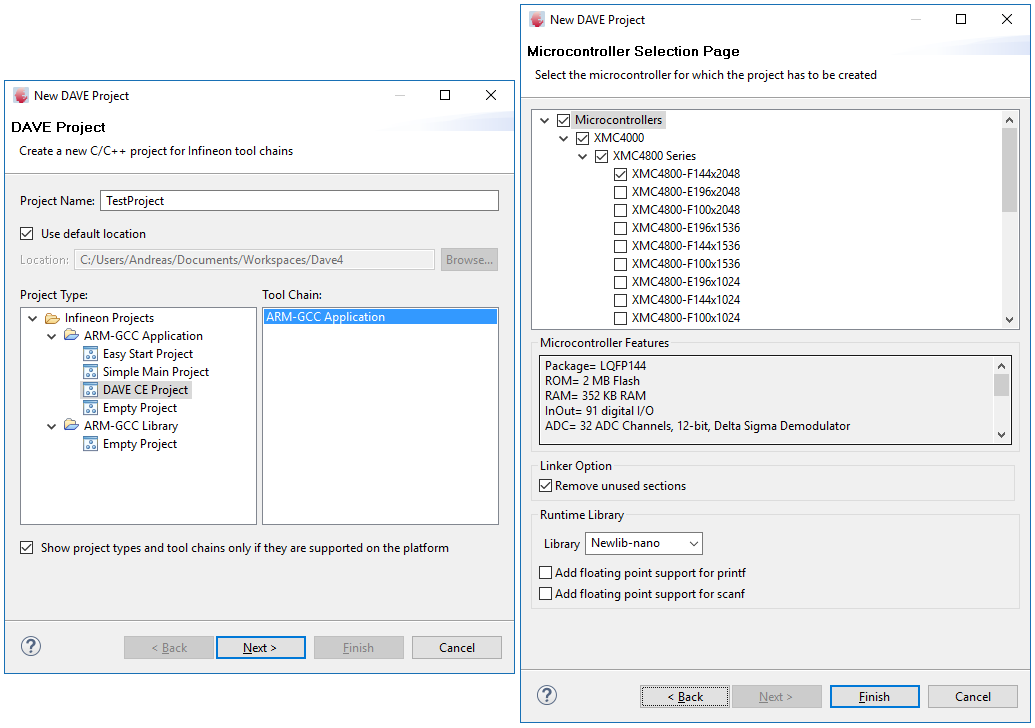
\includegraphics[width=\textwidth]{sensor/dave_project.PNG}
\caption{Projektdialog DAVE}
\label{img:dave_project}
\end{figure}

Einen Sonderfall bei den zur Auswahl stehenden Projektvorlagen stellen \textbf{DAVE CE} Projekte da. Diese Art von Projekt, ermöglicht die Verwendung von grafischen Oberflächen für die Konfiguration der Hardwareabstraktion. Dies umfasst unter anderem die Verbindung einzelner Komponenten untereinander oder mit den Pins des Mikrocontrollers, sowie grafische Konfigurationsformulare für die Komponenten selbst (z.B. ADC, CCU, POSIF, DIO usw.). \\ \\
Nach Wahl des Projektnamens und des gewünschten Projekttyps, muss auf der zweiten Seite des Dialogs der verwendete Mikrocontroller ausgewählt werden, um die korrekte Hardwarebibliothek bereitstellen zu können. Ein exemplarisches Beispiel für die Projekterstellung befindet sich in Abbildung \ref{img:dave_project}. 

\subsubsection{Projekt erstellen und herunterladen}
Um ein zu testendes Projekt auf den Controller herunterzuladen, muss es erst \textbf{kompiliert} werden. Gestartet wird der Buildprozess über den in Abbildung \ref{img:dave_build} markierten Button in der Menüleiste. 

\begin{figure}[ht]
\centering
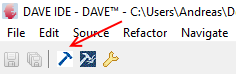
\includegraphics{sensor/dave_build.PNG}
\caption{Buildprozess starten}
\label{img:dave_build}
\end{figure}

\noindent
Im Anschluss an einen erfolgreichen Erstellungsprozess wird eine \textbf{Debug- bzw. Run-Konfiguration} angelegt. Diese umfasst alle für das Flashen benötigten Parameter wie Ort der zu ladenden Binärdatei sowieso GDB Konfigurationen.\\

\noindent
\fbox{\parbox{\linewidth}{Es ist wichtig, dass das Projekt vor dem Anlegen der Konfiguration einmal erstellt wird, da sonst wichtige Parameter nicht automatisch eingetragen werden.}} \\

\noindent
Das exemplarische Anlegen einer Debug-Konfiguration wird in Abbildung \ref{img:dave_debugConfig} gezeigt. Dafür wird im Fenster \textit{Debug Configurations} durch Doppelklick auf den eingesetzten Debug-Chip automatisch eine fertige Konfiguration angelegt.

\begin{figure}[ht]
\centering
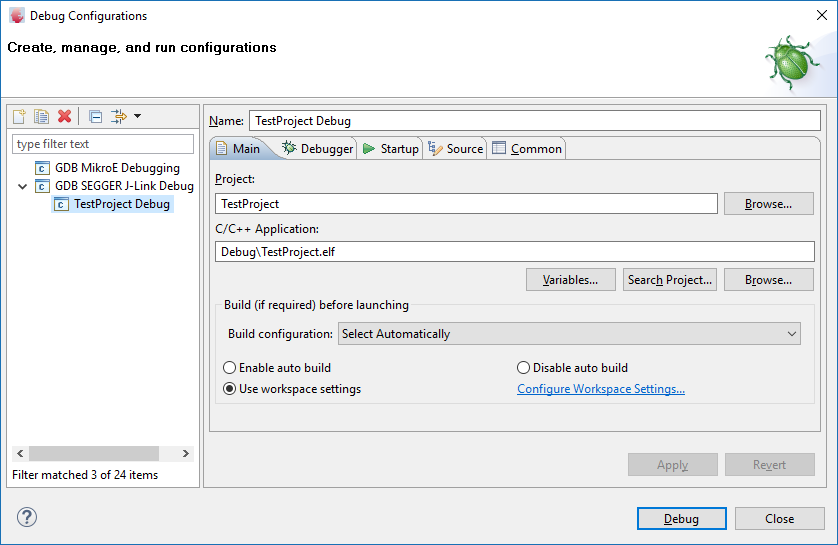
\includegraphics[width=0.8\textwidth]{sensor/dave_debugConfig.PNG}
\caption{Debug-Konfiguration erstellen}
\label{img:dave_debugConfig}
\end{figure}

\paragraph{Wichtiger Hinweis!} Es kann vorkommen, dass aus bisher unbekannten Gründen falsche GDB Startup-Skripte generiert werden, die beim Versuch das Projekt zu Debuggen, den sofortigen Abbruch des Vorgangs zur Folge haben. Es muss Sichergestellt werden dass in der Debug-Konfiguration, im Tab \textit{Startup}, unter dem Punkt \textit{Run/Restart Commands} keine Anweisungen eingetragen sind! \\

\noindent
Nach dem eine korrekte Konfiguration erstellt ist, kann das Programm über den Debug-Button in der Menüleiste auf den Controller geladen werden. DAVE wechselt im Anschluss automatisch in die Debug-Ansicht und unterbricht die Ausführung bei der ersten Anweisung in der Main-Funktion.

\subsection{POSIF}
\label{lbl:sensor_posif}
Das POSIF Modul der XMC Controller ist eigens auf den Betrieb von Motoranwendungen zugeschnitten. Dabei übernimmt es, in Kooperation mit einigen Capture Compare Units, den kompletten Workflow vom einlesen verschiedener Sensoren für die Bestimmung der Kommutierungszeitpunkte bis hin zur Ansteuerung des Motors, bzw. dem setzen der Ausgänge um die Spulen anzusteuern. Ein allgemeiner Aufbau befindet sich in Abbildung \ref{img:posif_overview}.

\begin{figure}[ht]
\centering
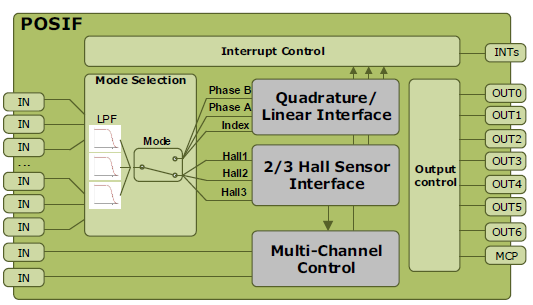
\includegraphics[width=0.8\textwidth]{sensor/posif_overview.PNG}
\caption{POSIF Übersicht}
\label{img:posif_overview}
\end{figure}

Im Wesentlichen verfügt das POSIF Modul über zwei verschiedene Betriebsmodi zum einlesen des Zustands, die Optional mit dem Modul für die Motoransteuerung kombiniert werden können.

\begin{itemize}
\item \textbf{Hall Modus} \\
In diesem Betriebsmodus werden dem POSIF Modul die Signalpegel der Hall-Sensoren zugeführt. Wird eine Änderung detektiert, wird das gemessene Pattern, automatisch mit dem erwarteten verglichen und es wird entweder ein Interrupt für ein \textit{Correct-Hall-Event} oder ein \textit{Wrong-Hall-Event} ausgelöst. In der Interruptroutine muss im Code das Register für das aktuelle und erwartete Hall-Pattern aktualisiert werden, um den reibungslosen Betrieb zu ermöglichen.
\item \textbf{Quadrature Decoder Modus} \\
Dieser Modus verwendet als Informationsquelle einen Inkrementalgeber, der eine Indexleitung, sowie zwei Phasen A und B bereitstellt (alternativ kann auch ein Encoder mit nur \textit{Direction-} und \textit{Count-Leitung} verwendet werden). Unter Zuhilfenahme einer kompletten CCU lassen sich sowohl Umdrehungsgeschwindigkeit als auch Drehwinkel berechnen.
\end{itemize}

\section{Sensor Interface}
Sämtliche Funktionen die das Auslesen der definierten Sensorwerte ermöglichen sollen, sind in ein eigenes Softwaremodul gekapselt, dass die gewünschte Funktionalität über festgelegte Schnittstellen anbietet. \\

\begin{lstlisting}[frame=single, language=c, caption=Sensor Interface, label=lst:SensorInterface]
void Sensor_Init();

void Sensor_StartAll(void);

void Sensor_StopAll(void);

void Sensor_SetDirection(MotorDirection_t direction);

Std_ReturnType Sensor_RegisterHallCallback(HallCallbackType callback);

Std_ReturnType Sensor_GetCurrentHallPattern(HallPattern_t* pattern);

Std_ReturnType Sensor_GetVelocity(double* velocity);

Std_ReturnType Sensor_GetAngle(double* angle);

Std_ReturnType Sensor_GetTemperature(int* temperature);
\end{lstlisting}

\subsection{Modulstruktur}
Das angebotene Interface über die Sensor.h Datei, fungiert nur als Schnittstelle zu den Implementierungen der einzelnen Sensoren. Die Aufteilung in Submodule leitet sich dabei aus den verschiedenen Sensortypen her. \\
\dirtree{%
.1 Sensor.
.2 Sensor\_Types.h.
.2 Sensor\_Hall.h.
.2 Sensor\_QuadratureDecoder.h.
.2 Sensor\_Temperature.h.
}
\noindent \\
Alle Submodule bringen zum jetzigen Zeitpunkt ihre Abhängigkeiten\footnote{Mit Abhängigkeiten sind in erster Linie Konfigurationen der Hardwareelemente wie CCU, ADC oder POSIF gemeint.} schon mit, um den Integrationsaufwand in das fertige Projekt so gering wie möglich zu halten. Dies kann sich zu einem späteren Zeitpunkt noch ändern, wenn die POSIF Konfiguration für das einlesen der Hall-Sensoren mit der Motorsteuerung zusammengezogen wird, da beide Module auf dieselbe Hardwarekomponente zugreifen.

\subsection{Anwendung}
Um Sensorwerte über das Softwaremodul einzulesen muss beim Startvorgang der Steuerung einmal die \textit{Sensor\_Init()} Funktion aufgerufen werden um alle eingesetzten Hardwarekomponenten zu initialisieren. Zu diesem Zeitpunkt sollte auch ein Callback für die Hall-Events registriert werden, um über eintretende Änderungen der Motorwelle informiert zu werden. Registrieren lässt sich eine Callback-Funktion über \textit{Sensor\_RegisterHallCallback(<func\_ptr>)}. \\
Vor dem Start muss dem Sensormodul ebenfalls die gewünschte Drehrichtung des Motors, über die Funktion \textit{Sensor\_SetDirection(<motor\_dir>)} mitgeteilt werden, um das korrekte Hall-Pattern ermitteln zu können. \\
Der Einlesevorgang für die Sensorwerte muss im Anschluss über die Funktion \textit{Sensor\_StartAll()} gestartet werden, und lässt sich über \textit{Sensor\_StopAll()} anhalten. \\

\noindent
Während des Regelbetriebs lassen sich die einzelnen Werte über die restliche API auslesen.

\begin{itemize}
\item \textbf{Sensor\_GetCurrentHallPattern(HallPattern\_t*)} Gibt das Muster zurück, dass sich durch den aktuellen Zustand der digitalen Hall-Sensoren ergibt. HallPatter\_t* beschreibt dabei einen Pointer auf die Hall-Pattern Struktur die durch den Funktionsaufruf mit Werten gefüllt wird.
\item \textbf{Sensor\_GetVelocity(double*)} Gibt die aktuelle Umdrehungsgeschwindigkeit der Motorwelle in Umdrehungen pro Sekunde zurück.
\item \textbf{Sensor\_GetAngle(double*)} Gibt den aktuellen Drehwinkel in Grad, relativ zu einem festgelegten Nullpunkt zurück.
\item \textbf{Sensor\_GetTemperature(int*)} Gibt die aktuelle Temperatur in Grad Celsius im Motor zurück.
\end{itemize}

\section{Hall Sensoren}
Ein Hall-Sensor misst magnetische Flussdichte, durch die Ausnutzung des Hall-Effekts. In unserem Versuchsaufbau sind drei dieser Sensoren, jeweils im Winkel um 120$^\circ$ versetzt, im Motor verbaut (Abbildung \ref{img:hall_sample}). Es handelt sich dabei um digitale Sensoren, was bedeutet, dass der gemessene Sensor-Wert entweder logisch 1 oder 0 ist.

\begin{figure}[ht]
\centering
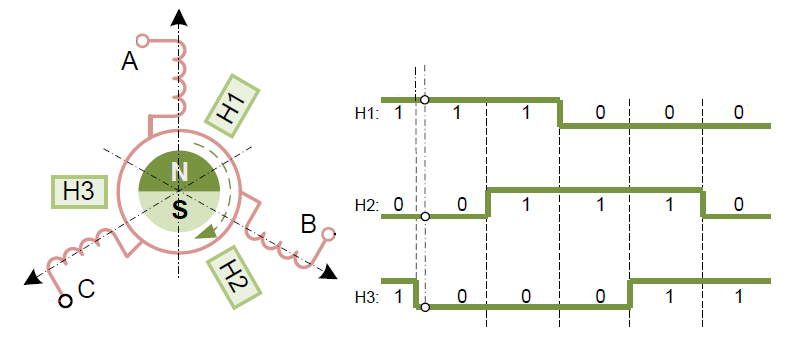
\includegraphics[width=0.8\textwidth]{sensor/hall_sample.PNG}
\caption{Hall Sensoren und Pattern}
\label{img:hall_sample}
\end{figure}

Der Wert ändert sich dabei in Abhängigkeit davon, ob sich grade ein magnetischer Nord- bzw. Südpol über den Sensor befindet. Alle drei Sensorzustände zusammen genommen ergeben ein \textbf{Hall-Pattern}, was im rechten Teil von Abbildung \ref{img:hall_sample} noch einmal verdeutlicht wird. Das Hall-Pattern ist relevant für zwei Dinge. Zum einen kann Anhand des gemessenen und des erwarteten Patterns festgestellt werden, ob beim Drehvorgang Fehler aufgetreten sind (z.B. ob der Motor sich in die falsche Richtung dreht) und zum anderen lässt sich aus dem Zeitpunkt des Auftretens einer Änderung des Musters, eine passende Gelegenheit für die Kommutierung ableiten. Bei gewissen Regelstrategien lässt sich außerdem aus dem Hall-Pattern ein Motor-Pattern ableiten, welches an die Spulen angelegt wird um eine Drehung des Motors zu erzeugen.

\subsection{Einlesen der Hall-Sensoren}
Die für uns effizienteste Möglichkeit das Hall-Pattern einzulesen und seine Korrektheit zu prüfen ist die Verwendung des in Kapitel \ref{lbl:sensor_posif} beschriebenen POSIF Moduls (POSition InterFace), dass die Verwendeten XMC Mikrocontroller mitbringen.\\

\noindent
In der verwendeten Konfiguration benötigt der Hall-Modus zwei CCU Slices. Wird vom POSIF Modul die Änderung der Eingänge detektiert, startet es das erste CCU Slice als Debounce Timer, um auszuschließen, dass die Statusänderung ihren Ursprung in einem Fehlerhaften Signal hat. Anschließend erfolgt der Vergleich, mit dem im Register abgelegten erwarteten Pattern, was entweder die Generierung eines Correct-Hall-Events oder Wrong-Hall-Events zur Folge hat. Im Fall eines CHE, löst die Software das registrierte Hall-Callback aus, um die Motorsteuerung über das eingetretene Ereignis zu benachrichtigen. Ebenfalls wird im Anschluss daran, das Register für das nächste erwartete Hall-Pattern aktualisiert. Das zweite CCU Slice kann verwendet werden, um auf Basis der auftretenden Hall-Events die aktuelle Umdrehungsgeschwindigkeit bzw. den Winkel der Motorwelle zu berechnen.

\subsection{Ermittlung der Hall-Pattern}
Der reibungslose Betrieb des Hall Moduls im Sensor Interface setzt voraus, dass das Register des POSIF Moduls immer mit dem korrekten, erwarteten Hall-Pattern befüllt wird. Dieses Muster unterscheidet sich je nach verwendetem Motor, und musste in unserem Fall extra ausgemessen werden. Dazu habe ich die Hall-Sensoren mit Spannung versorgt und an jede der drei Leitungen ein Oszilloskop gehängt. Durch händisches Drehen des Motors wird die gewünschte Abfolge sichtbar (abgebildet in Abbildung \ref{img:hall_pattern}).

\begin{figure}[ht]
\centering
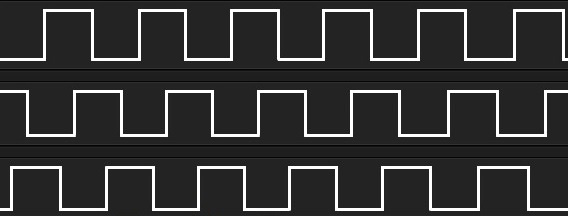
\includegraphics[width=0.8\textwidth]{sensor/hall_pattern.jpg}
\caption{Eingelesenes Hall-Pattern}
\label{img:hall_pattern}
\end{figure}

Auf Basis dieser Messung lässt sich durch festlegen eines beliebigen Startpunkts das Hall-Pattern für die gewählte Drehrichtung ableiten. Ab dem gewählten Startpunkt führt jede Änderung des Zustands zu einem neuen Pattern. Die Analyse hat für unseren Motor hat 6 verschiedene Pattern ergeben, die sich pro Umdrehung 7-Mal wiederholen. Dies ergibt eine Gesamtzahl von 42 Hall-Events pro Umdrehung. Das gleiche Verfahren wurde zu Überprüfungszwecken auch mit der zweiten Drehrichtung durchgeführt, um Fehler zu vermeiden. 

\begin{figure}[ht]
\centering
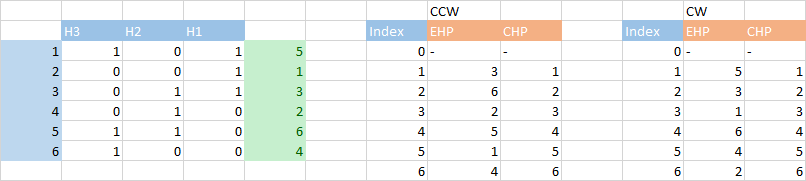
\includegraphics[width=\textwidth]{sensor/hall_pattern_lookup.PNG}
\caption{Hall-Pattern Lookup-Tables}
\label{img:hall_pattern_lookup}
\end{figure}

Um einen effizienten Wechsel der Pattern zu garantieren, wird eine Lookup-Table eingesetzt, die das aktive Hall-Pattern als Index nutzt, um das nächste erwartete Pattern zu finden. Die genaue Struktur der Tabelle ist in Abbildung \ref{img:hall_pattern_lookup} aufgeschlüsselt.

\section{Inkrementalgeber}
Für die Berechnung der Umdrehungsgeschwindigkeit und des aktuellen Winkels steht ein Inkrementalgeber zur Verfügung, der über eine Indexleitung Z und zwei Phasen A und B verfügt. Der Sensor selbst ist mit der Motorwelle gekoppelt und verändert seine Leitungspegel mit den Drehbewegungen der Welle. \\

Die Umdrehungsgeschwindigkeit lässt sich über die Indexleitung errechnet, die pro vollständiger Umdrehung der Welle an einem definierten Punkt für kurze Zeit einen High-Pegel annimmt. Der Winkel sowie die Drehrichtung lassen sich über die Phasen A und B ermitteln. Wie in Abbildung \ref{img:quadrature_overview} gezeigt, wechseln sowohl A als auch B immer zwischen einem High- und Low-Zustand. Da nicht beide Phasen gleichzeitig den Pegelwechsel vollziehen, sondern je nach Drehrichtung eine Phase vor der anderen, lässt sich daraus die Drehrichtung ableiten. Den aktuellen Winkel erhält man durch Mitzählen, da pro Umdrehung immer die gleiche definierte Anzahl an Flankenwechsel durchgeführt werden. Der absolute Winkel, relativ zum Nullpunkt den die Indexleitung vorgibt, erhält man durch die Formel \ref{eq:angle}.

\begin{equation}
\label{eq:angle}
angle = (edge_count / total_edges) * 360
\end{equation}

\begin{figure}[ht]
\centering
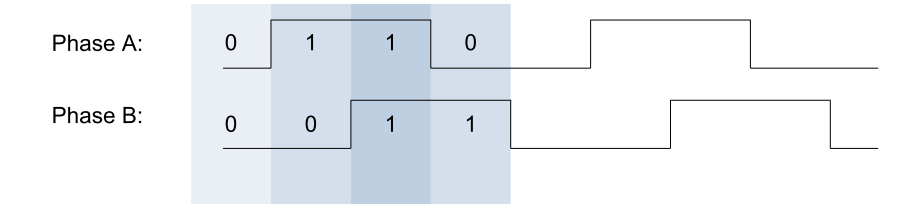
\includegraphics[width=\textwidth]{sensor/quadrature_overview.PNG}
\caption{Inkrementalgeber Phasen}
\label{img:quadrature_overview}
\end{figure}

\subsection{Implementierung}
Für das Einlesen und die Verarbeitung der Leitungssignale des Inkrementalgebers wird das im Kapitel \ref{lbl:sensor_posif} beschriebene POSIF Modul im Quadrature Decoder Modus herangezogen. Durch zuführen der Phasen und der Indexleitung errechnet die verwendete POSIF Instanz sechs verschiedene Ausgänge. 

\begin{itemize}
\item Auftreten des Indexsignals
\item Fertige Umdrehung
\item Drehrichtung
\item Quadrature Clock
\item Period Clock
\item Synchronisierter Start
\end{itemize}
 
In Kombination mit passend konfigurierten CCU Slices lassen sich Anhand der internen Ausgänge des POSIF Moduls die angestrebten Kenngrößen ermitteln.

\section{Temperatursensor}
Der eingesetzte Sensor für die Ermittlung der Temperatur im Motor verwendet einen NTC-Widerstand (Negative Temperature Coefficient) für die Temperaturermittlung. Bei dieser Bauform, sinkt der Widerstand des Sensors bei steigender Temperatur. Die bei uns verbaute Variante deckt einen Temperaturbereich von -40$^\circ$ bis 110$^\circ$ Celsius ab und verfügt über einen Basiswiederstand von 10kOhm bei einer Temperatur von 25$^\circ$ Celsius.

\subsection{Einlesen des Temperaturwerts}
Für die Ermittlung des aktuellen Temperaturwerts ist es notwendig den Widerstandswert des Sensors einzulesen und zu digitalisieren. Da sich der Widerstand nicht direkt messen lässt wird ein Spannungsteiler eingesetzt, dessen Spannung am Messpunkt sich proportional zum Widerstand verhält. Diese Messspannung kann am Controller über einen AD-Wandler eingelesen werden.

\begin{figure}[ht]
\centering
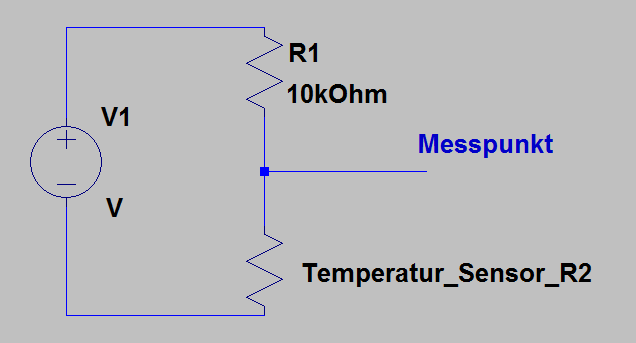
\includegraphics[width=0.65\textwidth]{sensor/temperature_circuit.PNG}
\caption{Spannungsteiler zum einlesen des NTC-Widerstands}
\label{img:temperature_circuit}
\end{figure}

Der genaue Schaltungsaufbau lässt sich aus Abbildung \ref{img:temperature_circuit} entnehmen. Als fixer Widerstand werden 10kOhm verwendet. Dieser Wert spielt später bei der Errechnung des Widerstands des Temperatursensors T1 eine Rolle. Nach Anlegen einer Versorgungsspannung lässt sich die variable Spannung am Messpunkt abgreifen. \\
\label{lbl:temp_equation}
Um aus der gemessenen Spannung den Widerstand zu errechnen, muss zunächst von der Formel für $U_{2}$ des Spannungsteiler ausgegangen werden.

\begin{equation}
U_{2} = \frac{U_{ges}}{R_{1} + R_{2}} * R_{2}
\end{equation}

Bekannt sind in dieser Formel die Werte für $U_{ges}$, die gemessene Spannung $U_{2}$ und der Widerstand $R_{1}$. Durch Äquivalenzumformung lässt sich die Formel auf den gewünschten Wert $R_{2}$ umstellen.

\begin{equation}
R_{2} = \frac{U_{2} * R_{1}}{U_{ges} - U_{2}}
\end{equation}

Ist der Widerstand bekannt, lässt sich aus dem Datenblatt des Sensors die dazu passende Temperatur ermitteln.

\subsubsection{Analog Digital Wandlung}
Die ADC Einheit des XMC Controllers verfügt über vier unabhängige Konvertierungsgruppen mit bis zu 8 analogen Eingängen und einer maximalen Auflösung von 12 Bit. Standard Referenzspannung sind dabei 3.3 Volt.

\begin{figure}[ht]
\centering
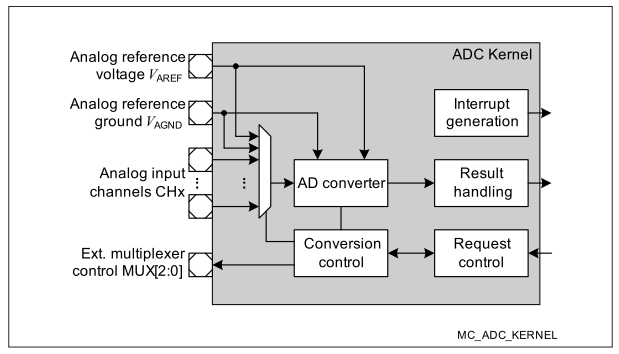
\includegraphics[width=0.9\textwidth]{sensor/xmc_adc.PNG}
\caption{ADC Einheit der XMC Controller}
\label{img:xmc_adc}
\end{figure}

Für die Wandlung stehen drei verschiedene Modi zur Verfügung: 
\begin{itemize}
\item \textbf{Fixed Channel Conversion} \\
Ein einzelner festgelegter Kanal wird konvertiert.
\item \textbf{Auto Scan Conversion} \\
Alle verfügbaren Kanäle werden in einer konfigurierbaren Sequenz automatisch und linear gewandelt.
\item \textbf{Channel Sequence Conversion} \\
Konvertierung von 8 willkürlich gewählten Kanälen.
\end{itemize}
%todo heißt das Arbiter im folgendem Kapitel??
Jeder dieser Modi kann entweder einmalig auf explizite Anfrage, oder kontinuierlich eine Konvertierung durchführen. Als Quelle der Anfragen stehen ebenfalls mehrere Einheiten zur Verfügung (zwei Group-Request-Sources und eine Background-Request-Source). Da von mehreren Quellen Anfragen gleichzeitig eintreffen können, wird die Reihenfolge der Abarbeitung von einem Arbiter festgelegt. Der genaue Aufbau einer einzelnen ADC Einheit lässt sich der Abbildung \ref{img:xmc_adc} entnehmen. \\

In unserem konkreten Beispiel wird eine Fixed-Channel-Konvertierung durchgeführt, da nur ein einzelner Kanal eingelesen werden muss. Das Absetzen der Anfrage wird dabei von der Background-Request-Source übernommen. Da die Konvertierung einige Mikrosekunden Zeit benötigt, wird nach Abschluss des Vorgangs ein Interrupt ausgelöst.

\subsubsection{Implementierung}
Die Ermittlung des aktuellen Temperaturwerts wird nur auf Anfrage durch die Sensor API ausgeführt. Die im Codesnippet \ref{lst:temp_calculation} aufgeführte Funktion, startet die Konvertierung und wartet durch Busy-Waiting auf deren Abschluss. Zu dem gemessenen Spannungswert wird wie bei \ref{lbl:temp_equation} aufgeführt, der zugehörige Widerstandswert berechnet. Der passenden Temperaturwert wird durch die Suche in einer sortierten Tabelle ermittelt.

\begin{lstlisting}[frame=single, language=c, caption=Temperaturberechnung, label=lst:temp_calculation]
int Sensor_Temperature_Calculate(Sensor_TemperatureType sensor)
{
	int i = 0;
	double adcVoltage = 0;
	double res = 0;

	/* Start measurement */
	MeasurementRunning = 1;
	Sensor_Temperature_ADC_StartConversion();

	/* Wait for measurement to finish*/
	while(MeasurementRunning == 1);

	/* Calculate temperature */
	adcVoltage = ConvertToVoltage(SensorVoltages[sensor]);
	res = (adcVoltage * R1) / (SENSOR_REF_VOLTAGE - adcVoltage);

	while(TemperatureLookupTable[i++].resistence > res && 
			i < NTC_LOOKUP_ENTRIES);

	return TemperatureLookupTable[i].temperature;
}
\end{lstlisting}

\section{Ausblick}
Momentan befindet sich der Code für das Einlesen der Sensorwerte vom Inkrementalgeber noch in Entwicklung. Bei der aktuellen Bearbeitungslage ist eine vollständige Fertigstellung nicht absehbar. \\
Basierend auf der Ideensammlung aus der Analysephase wäre eine mögliche Erweiterung dieses Arbeitspakets die Portierung auf andere Controller. Durch das mögliche Fehlend des POSIF Moduls auf anderen Plattformen wird dadurch eine Neuimplementierung für das Einlesen der Hall-Sensoren sowie des Inkrementalgebers notwendig. \\ \\
Eine weitere Aufgabe wäre die Kommutierung nicht von den Hall-Events abhängig zu machen, sondern als Basis den Inkrementalgeber zu verwenden. Dies ermöglicht die Verwendung neuer Kommutierungsstrategien und stellt mit Sicherheit eine interessante Erweiterung des Funktionsumfangs da.

\graphicspath{{./regulation/}}
\chapter{Arbeitspaket Regelung}
Für die Analyse, Entwurf, Implementierung und Integration dieses Arbeitspaketes übernahm Herr Krupinski die Verantwortung.
\paragraph{}
Die Regelung stellt im wesentlichen ``Glue-Code'' für die Kommunikation, Motorsteuerung und Sensorik bereit. Dabei ist der Kern eine Implementierung eines PID(proportional–integral–derivative)-Regler.
\section{Analysephase}
\subsection{Hardware}
Für die Regelung ist es möglich die Programmierung nahezu Hardware unabhängig zu realisieren. Dafür müssen die $\mu$-Controller abhängigen Komponenten (Kommunikation, Motorsteuerung und Sensorik) über ein Interface abstrahiert werden. Die Regelung ``kennt'' und kommuniziert nur gegen diese Interfaces, was es ermöglicht die spezifischen Implementierungen jederzeit austauschen zu können, ohne die Regelung erneut ändern zu müssen.\\
Da für den I- und D-Anteil der Regelung allerdings eine relative Zeit benötigt wird, ist es nicht komplett möglich $\mu$-Controller unabhängig zu entwickeln. Um diese relative Zeit messen zu können, müssen Timer-Komponenten der Hardware genutzt werden. Die einzige Möglichkeit dies zu vermeiden, wäre eine Annahme zu treffen, wie viel Zeit seit der letzten Iteration vergangen ist.
\paragraph{}
\subsection{Software}
Der Motor soll auf verschiedene Werte hin gesteuert werden können. Zum Beispiel auf eine bestimme Drehzahl oder Drehmoment. Grundsätzlich ist dies davon abhängig, welche Werte der Controller über die Sensorik lesen und welche Werte über die Motorsteuerung direkt, oder indirekt beeinflusst werden können. Deshalb muss es möglich sein ohne großen Aufwand die Regelung auf mehrere Werte zu erweitern, beziehungsweise grundsätzlich dafür entworfen sein. Zusätzlich müssen diese Parameter zur Laufzeit, über die Kommunikations-Schnittstelle, verändert werden können. Konkret die Einflussfaktoren der P-, I- und D-Anteile, Zielwert und zu regelnden Wert.

\section{Entwurfsphase}
Hauptteil des Entwurfs bestand aus der konkreten Definition der Interfaces zwischen Regelung und Kommunikation/Motorsteuerung/Sensorik.
\section{Implementierung}
\section{Integration}
\section{Ausblick}


\chapterauthor{Ricardo Krause}
\graphicspath{{./gui/Bilder/}}

\chapter{Arbeitspaket GUI}
\label{GUI}
Für die Analyse, den Entwurf und die Implementierung dieses Arbeitspaketes übernahm Herr Krause die Verantwortung. Er wurde bei der Implementierung von den selbst erstellten Steuerelementen vom Herrn Krupinski unterstützt. Während der Integration des Arbeitspaketes waren die Herren Krupinski und Schleinkofer unterstützend beteiligt.
\paragraph{}
In der Projektspezifikation wurde die Anforderung der Visualisierung von Motor-Charakteristiken und die Steuerung des Motors mit aufgenommen. Zu diesem Zweck wurde eine Benutzeroberfläche in der Programmiersprache C\# mit Hilfe des Grafik-Framework\footnote{Rahmenstruktur in der Software} \textit{WPF} \footnote{Windows Presentation Foundation} von Microsoft erstellt.

\section{Analysephase}
Das Arbeitspaket GUI wurde mit einer Analysephase begonnen. In dieser Phase wurden die möglichen funktionalen und nicht-funktionalen Anforderungen in einer Spezifikation zusammengetragen und aufgelistet. Es wurden Stakeholder\footnote{Projektbeteiligte, welche nicht an der Entwicklung beteiligt sind} befragt, um die gewünschten Anforderungen an das System zu erhalten und anschließend wurden die Ergebnisse der Befragung validiert, priorisiert und in die Spezifikation mit aufgenommen. Die umzusetzenden Projektinhalte wurden dann aus dieser abgleitet.\\
Die wichtigsten drei Anforderungen jeder Gruppe, basierend auf der Analyse: \\

\begin{minipage}[t]{0.4\textwidth}
\textbf{Funktionale Anforderungen:}
\begin{itemize}
	\item Anzeige von Sensordaten in der GUI
	\item Einstellung möglicher Parameter des Motors
	\item Justierung der PID Regelung in der GUI
	\end{itemize} 
\end{minipage}\hfill\begin{minipage}[t]{0.5\textwidth}
\textbf{Nicht-Funktionale Anforderungen:}
\begin{itemize}
	\item Die Software soll Modular aufgebaut und erweiterbar sein
	\item Es soll das aktuelle Metro-Design verwendet werden
	\item Der Aufbau soll möglichst einfach gehalten sein, um die Stabilität und Benutzbarkeit zu verbessern.
\end{itemize} 
\end{minipage}
\newline
\newline
\newline
Als weiteres Ergebnis der Analyse ergab sich eine zwingende Abhängigkeit zu dem Arbeitspaket Kommunikation, wo die erforderlichen Schnittstellen und Datenstrukturen in enger Zusammenarbeit erstellt wurden. Diese sind ebenfalls in die Spezifikation mit aufgenommen worden.
\section{Entwurfsphase}
Mit den Ergebnissen der Analysephase, wurde ein Entwurf der Benutzeroberfläche erstellt. Dieser wurde auf der einen Seite für die Code Struktur und Architektur durchgeführt, auf der anderen Seite wurden mögliche Designentwürfe des Layouts erstellt.\\

Als grundlegende Architektur wurde ein drei Schichtenmodell \ref{fig:arc} verwendet, welches den Anforderungen der Analysephase gerecht wird und allen Entwicklern des Projektes bekannt ist. In diesem gewählten Modell kommunizieren nur benachbarte Schichten miteinander. Und jede Schicht hat eine separate Aufgabe.

\begin{figure}[ht]
	\centering
		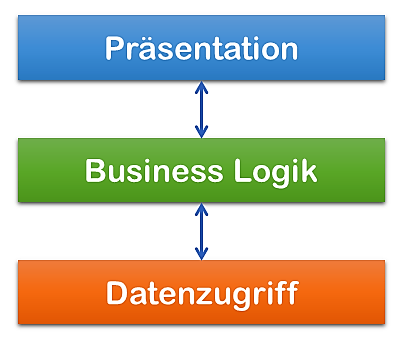
\includegraphics[scale=0.5]{Arc1}
		\caption{Grober Architektur Entwurf}
		\label{fig:arc}
\end{figure}

Es wurden mehrere Entwurfsmuster verwendet, welche zur Softwarequalität beitragen und dem Entwickler einzelne Lösungsgerüste für wiederkehrende Probleme liefern.\\

Für die oberen beiden Schichten wurde das MVVM\footnote{kurzw. für Model-View-ViewModel} Entwurfsmuster \ref{fig:mvvm} gewählt. Dieses Muster trennt die Oberfläche von der zugrundeliegenden Business-Logik, dies ermöglicht es die Komponenten unabhängig und austauschbar von der Businesslogik zu entwickeln.\\ 

\begin{figure}[ht]
	\centering
		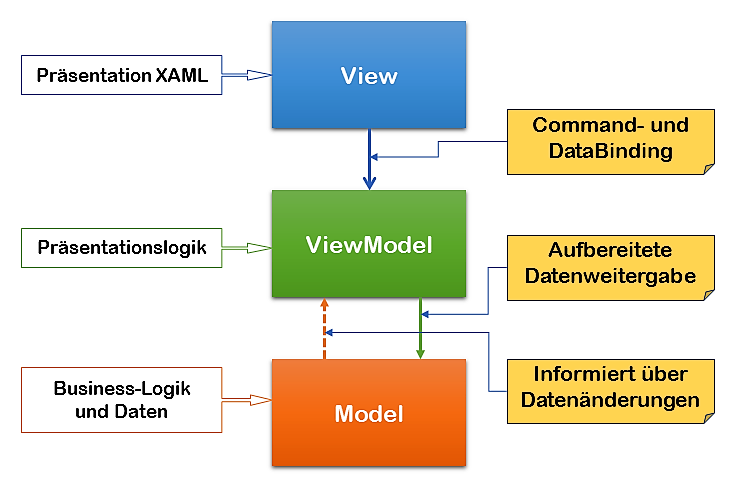
\includegraphics[width=0.6\textwidth]{MVVM}
		\caption{MVVM-Konzept}
		\label{fig:mvvm}
\end{figure}

Weitere eingesetzte Entwurfsmuster sind das Kommandomuster, welches alle ausgeführten Events auf der Benutzeroberfläche auffängt und im ViewModel behandelt und verarbeitet, das Repository\footnote{engl. Haufen}-Muster, welches die Daten Verwaltung und Kommunikation zu Subsystemen übernimmt und flexible auf Änderungen im Kommunikationsmodul reagiert und das "Umkehrung der Kontrolle"-Muster, für dessen Zweck ein Abhängigkeits-Container zu Beginn des Systemstarts erstellt und mit allen bekannten Abhängigkeiten gefüllt wird. Anschließend ist der Zugriff auf die im Container befindlichen Objekte von jedem Punkt der Anwendung her ermöglicht.\\

Wie bereits in der Analysephase erwähnt, wurden die Datenstrukturen dem Kommunikationsmodul angepasst siehe Abbildung \ref{lst:SensorData}.\\
\begin{lstlisting}[frame=single, caption=Beschreibung der Sensordatenstruktur, label=lst:SensorData]
public class SensorData
{
public ulong Timestamp { get; set; }
public SortedList<ushort, double> DataTable { get; set; }
}
\end{lstlisting}
Im zweiten Teil des Entwurfes wurde ein erstes einfaches Layout \ref{fig:gui} erstellt. Für dieses wurde das Werkzeug Pencil\footnote{Link zum Projekt \url{http://pencil.evolus.vn/}} eingesetzt. Es ist einfach zu bedienen und lieferte schnell ein Ergebnis, welches im Projektteam besprochen werden konnte.

\begin{figure}[ht]
	\centering
		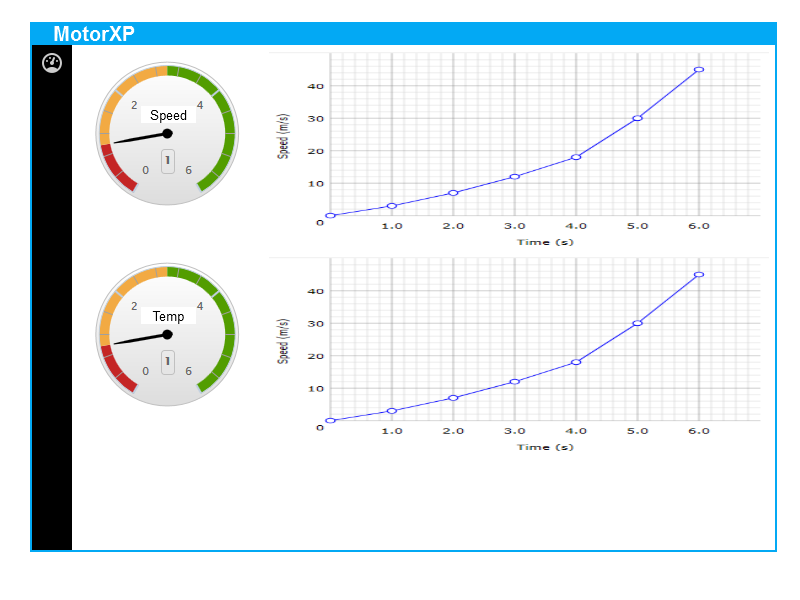
\includegraphics[width=0.5\textwidth]{Mockup}
		\caption{Erster Layout Entwurf der GUI}
		\label{fig:gui}
\end{figure}

\section{Implementierung}

In diesem Abschnitt werden wurden die Ergebnisse der Entwurfsphase umgesetzt und die Benutzeroberfläche erstellt. Das Programm wurde mit dem Visual Studio 2015 in der Programmiersprache C\# und den .NET Framework WPF erstellt. In dieser Phase kommen die vom Herrn Krupinski erstellten Steuerelemente zum Einsatz unterstützt.\\

Zu Beginn der Implementierung wurde die Frage aufgeworfen, welche Technologie für die Oberfläche zum Einsatz gebracht werden sollten. Zur Auswahl stand, es mit neuesten Multi-Plattform fähigen Web-Technologien umzusetzen und auf das ASP.NET-Framework\footnote{Microsoft Framework zur Entwicklung von Web-Applikationen} zu setzen oder eine reine Desktop Applikation mit dem WPF-Framework umzusetzen. Aufgrund des relativ knappen Zeitplanes für das Projekt und der mehrheitlichen Erfahrungen im WPF-Framework, wurde sich für dieses entschieden.\\

Als Entwicklungsumgebung wurde das Visual Studio Enterprise 2015 eingesetzt. Dieses Tool bietet dem Entwickler einen sehr kraftvollen Code-Editor, einfach zu bedienenden Debugger, umfangreiche Diagnose Tools, integriertes Test Framework und ist flexibel erweiterbar zusätzlich werden Projekt Templates bereitgestellt, welche schon grundlegende Konzepte wie Architektur Muster mitbringen.\\

Als Grundlage für den Start des Projektes wurde das MVVM-Light\footnote{Link zum Projekt\url{https://mvvmlight.codeplex.com/}} Toolkit verwendet. Es beinhaltet grundlegende Funktionalitäten und Templates, welche den Entwickler, indem es Basistechnologien wie die Architektur Struktur MVVM und DI-Techniken mitbringt, entlasten. Dieses Toolkit ist ebenfalls als Erweiterung direkt im Visual Studio verfügbar.\\

Der Datenzugriff wurde durch den Einsatz vom Repository-Muster (siehe Abbildung \ref{fig:repo}) realisiert. Dies ermöglichte zu Beginn des Projektes und für Test gegen eine Attrappe des Kommunikationsmoduls zu entwickeln. Diese täuschte das fehlende Modul vor und konnte problemlos durch das fertig implementierte Modul ersetzt werden. Durch die vorangegangene Schnittstellen Definition mussten für die Integration des Kommunikationsmoduls keine Änderungen an der internen Systemlogik vorgenommen werden.   

\begin{figure}[ht]
	\centering
		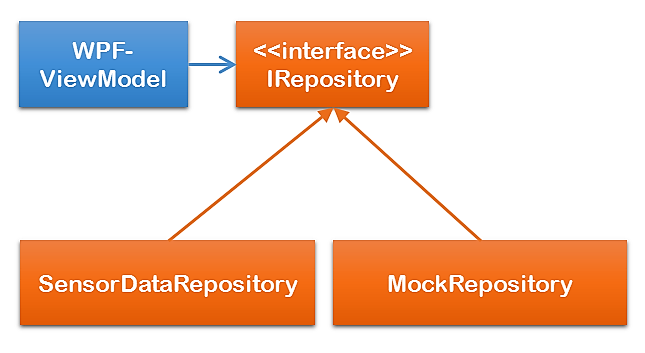
\includegraphics[width=0.5\textwidth]{RepoPattern}
		\caption{Repository Muster in der GUI}
		\label{fig:repo}
\end{figure}

Ein weiteres Problem, welches es zu lösen gab, waren die Steuerelemente für die Anzeige. Es folgte eine kurze Evaluation und Testphase für die möglichen Tachometer und Linienchart Anzeigen, leider mit dem Ergebnis, dass die fertigen Produkte entweder Kostenpflicht waren oder schlecht dokumentiert und nicht genügend Anpassbar für unseren Zweck waren.\\

Daraufhin erstellte der Herr Krupinski diese beiden aufwändigen Steuerelemente als Benutzerdefinierte WPF-Steuerelemente selbst, welche uns die geforderten Funktionalitäten und die notwendige Veränderbarkeit mitbrachten. 



\subsection*{Gauge Control}
Das entwickelte "Gauge"\footnote{Englisch für Tachometer.} Control in Abbildung \ref{fig:gauge} besteht aus einer Skala(1) mit einem minimal und maximal Wert, einen Zeiger(2) und einem Label(3), welches den Aktuellen Wert anzeigt.

\begin{figure}[ht]
	\centering
		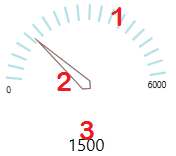
\includegraphics[width=0.3\textwidth]{Gauge1}
		\caption{Tachometer Anzeige der GUI}
		\label{fig:gauge}
\end{figure}

\subsection*{LineChart Control}

In Abbildung \ref{fig:line} ist das "LineChart"\footnote{Englisch für Liniendiagramm.} Control abgebildet. Es besteht aus einem anzeige Raster (1), einen Graphen (2) zur Visualisierung der Werte einer Anzeige für die Y-Achse (3) mit einstellbaren Werten und einer Anzeige für den ersten und letzten Wert der X-Achse (4).

\begin{figure}[ht]
	\centering
	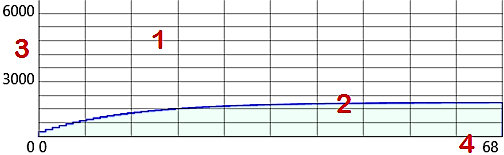
\includegraphics[width=0.6\textwidth]{Line1}
	\caption{Liniendiagramm Anzeige der GUI}
	\label{fig:line}
\end{figure}

\newpage

\subsection{Implementierung Gauge und Line Control}
\chapterauthor{Bernd Krupinski}
\subsection{Gauge Control Implementierung}

Die Implementierung der Gauge Control erfolgte in der Windows Presentation Foundation (WPF) über eine Custom Control. Zur Darstellung der Skala(1) und dem Zeiger(2) wurden jeweils ein Canvas verwendet. Ein Canvas stellt in WPF eine Zeichenoberfläche dar.\\



Das Control stellt eine Reihe an Variablen zur Verfügung. Diese ermöglichen es dem Entwickler das Control mit Hilfe von wenigen Zeilen Code stark anzupassen. 
\begin{figure}[ht]
	\centering
	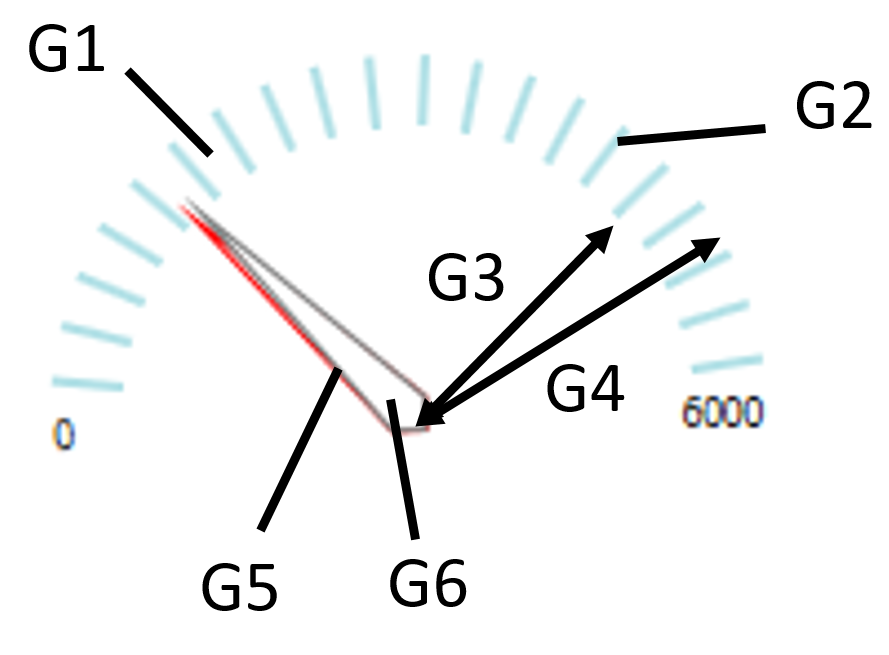
\includegraphics[width=0.6\textwidth]{GaugeDetails}
	\caption{Gauge Control Details}
	\label{fig:gauge}
\end{figure}
Umfassen dabei sind visuelle Parameter wie Kreishintergrundfarbe(G1), Strichlänge, Strichfarbe, Strichanzahl(G2), innerer Radius(G3), Nadellänge, Nadelfarbe(G6) oder Nadelfüllfarbe(G5). Zusätzlich dazu funktionelle Parameter wie Maximalwert, Minimalwert, aktueller Wert etc.\\\\

Das Canvas Control benutzt den Render Zyklus von WPF. Das heißt dass von unserer Seite das Canvas nur geändert werden muss, sollte einer der genannten Variablen sich verändern, also ein neu zeichnen des Tachometers notwendig ist.\\
Dies geschieht in 2 Schritten. \\
\begin{itemize}
	\item Zeichnen des Hintergrunds (Canvas 1)
	\item Zeichnen der Nadel (Canvas 2)
\end{itemize}

Der Hintergrund besteht wiederum aus 2 Teilen. \\

\begin{itemize}
	\item Der kreisförmige Hintergrund.
	\item Halbkreis aus Strichen.
\end{itemize}
Während die Striche mit einer Menge an Strich-Formen entlang des inneren Radius mit der Länge Äußerer Radius(G4) - Innerer Radius, einfach gelöst wird, stellt der Hintergrund eine etwas interessante Problematik.\\
Zwar gibt es eine Ellipsen Form für WPF's Canvas Control, allerdings besteht die Anforderung aus keiner rein einfarbigen Ellipse, sondern stattdessen aus einer zwei geteilte Form wie unten abgebildet.
\begin{figure}[ht]
	\centering
	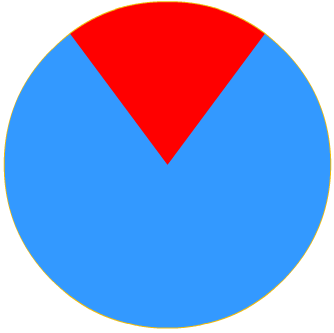
\includegraphics[width=0.6\textwidth]{GaugeForm}
	\caption{Gauge Control Details}
	\label{fig:gauge}
\end{figure}
Stattdessen wird ein Polygon benutzt. Ein Polygon ist eine mit einer Linie verbundene, Menge an Punkten. Optional kann die daraus entstehende Fläche mit einer Farbe gefüllt werden.\\
Um die gewünschte Form zu erzielen, werden 2 Polygone gezeichnet. Das eine (blau) umschließt das andere (rot) und bilden zusammen einen vollen Kreis.\\
\\
Die Nadel wird genau wie der Hintergrund über ein Polygon gezeichnet. Dabei wird die Nadel selbst auf dem Canvas stets richtung Osten gezeichnet. Damit die Nadel schließlich auf den entsprechenden Winkel zeigt, der den aktuellen Wert entspricht, wird nicht die Nadel schräg gezeichnet, sondern stattdessen das Canvas selbst über eine Rotations-Transformation gedreht.


\chapterauthor{Bernd Krupinski}
\subsection{LineChart Control Implementierung}
Das LineChart Control wurde ähnlich die das Gauge Control ebenfalls mit 2 Canvas in einer Custom Control in WPF geschrieben. 1 Canvas für den Hintergrund und Skala und 1 Canvas für den Graphen selbst.\\
Das Control ist wie das GaugeControl ebenfalls stark anpassbar. Diese Werte sind unter anderen vertikale Linien zeichnen, horizontale Linien zeichnen, Anzahl horizontale/vertikale Linien, Füllfarbe, Strichfarbe und mehr funktionale Variablen wie Mindestwert, Maximalwert, Fenstergröße, Fensterposition.\\
Für die genaue Erklärungen für jeden Wert siehe in-Code Dokumentation.
Das Control nimmt eine Menge an Punkten an und versucht diese so gut wie möglich darzustellen. Dabei kann das Control nur ein Fenster (Siehe Variablen Fenstergröße, Fensterposition) oder die gesamte Menge anzeigen.\\
Dies geschieht wieder über ein Polygon. Allerdings muss darauf geachtet werden, dass das Canvas eine variable Größe hat. D.h. der Graph muss relativ gezeichnet werden. Es entstehen zwei Fälle:\\
\begin{itemize}
	\item Es existieren mehr Pixel als Sample
	\item Es existieren mehr Sample (Punkte) als Pixel
\end{itemize}
Diese werden im Code unterschieden.\\
\newpage
Für den Fall mehr Pixel als Sample, wird durch jedes Sample iteriert und berechnet wie viele Pixel das momentane Sample entspricht. In der Abbildung entspricht jedes Sample mit Abstand von drei, zwei Pixel.\\
\begin{figure}[ht]
	\centering
	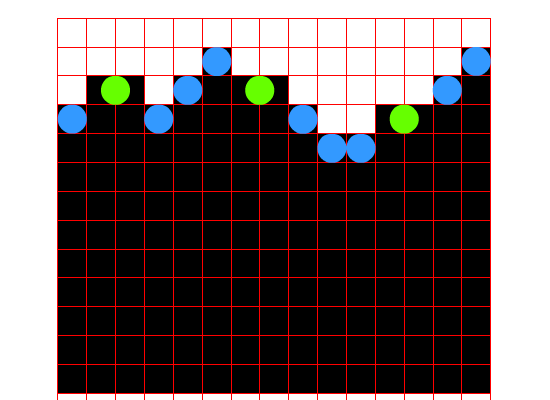
\includegraphics[width=0.6\textwidth]{TooFewSamples02}
	\caption{Beispiel: Mehr Pixel als Sample}
	\label{fig:gauge}
\end{figure}

Für den Fall mehr Sample als Pixel, wird wiederum durch jeden Pixel iteriert und berechnet welche Sample für das momentane Pixel relevant sind. Dabei werden stets 2 Pixel gleichzeitig betrachtet, da für die Darstellung das lokale Minimum und Maximum gezeichnet wird.\\

\begin{figure}[ht]
	\centering
	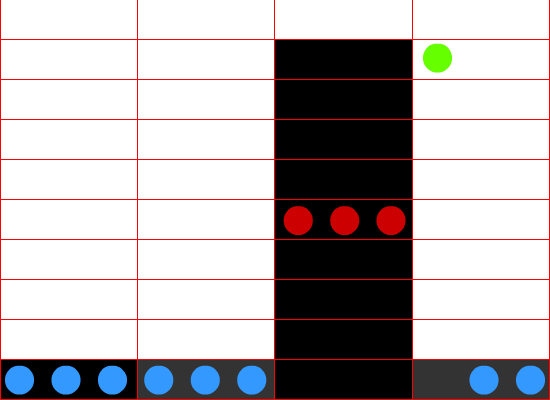
\includegraphics[width=0.6\textwidth]{TooManySamples030001}
	\caption{Beispiel: Mehr Pixel als Sample 01}
	\label{fig:gauge}
\end{figure}
In diese Abbildung zum Beispiel sind für die rechten zwei Pixel Spalten sechs Sample relevant. Drei rote Sample mit mittel hohen Wert, ein grünes Sample mit einem sehr hohen Wert und zwei blaue Sample mit niedrigen Werten.\\
Das Minimum und Maximum wird bestimmt. Das grüne Sample entspricht dem Maximum, während eins der blauen Sample das Mimimum entspricht. Da das Maximum (grün) rechts vom Minimum (blau) ist, wird entsprechend die linke Spalte das Maximum und die rechte Spalte das Minimum anzeigen.\\
\newpage
\chapterauthor{Ricardo Krause}
\subsection{Integration Controls}
Diese Steuerelemente bieten dem Entwickler diverse Einstellmöglichkeiten in Form und Farbgebung und sind beliebig erweiterbar für kommende Anforderungen. Die beiden Benutzer definierten Steuerelemente wurden zu einem eigenen Control zusammengefasst und mit weiteren Steuerelementen ergänzt. In Abbildung \ref{fig:control1} ist exemplarisch ein komplettes Anzeigeelement für einen Sensorwert abgebildet.

\begin{figure}[ht]
	\centering
		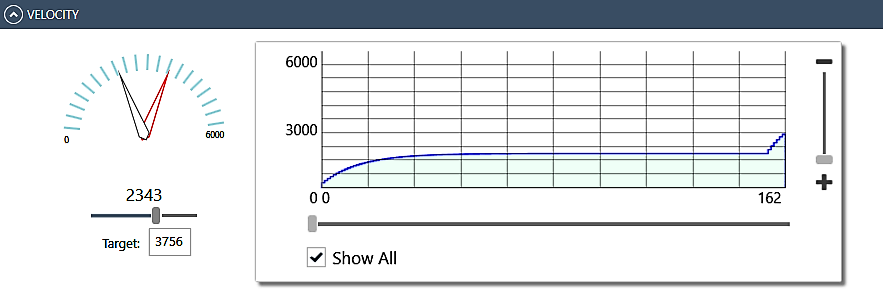
\includegraphics[width=\textwidth]{GUIScreenshot3}
		\caption{Datenanzeige Control}
		\label{fig:control1}
\end{figure}

Die Abbildung \ref{fig:guifinal} zeigt fertige die GUI zum Ende des Projektes. Sie ist aktuell in der Lage die definierten Sensorwerte anzuzeigen, die einzelnen Anzeigeelemente \ref{fig:control1} bieten die Möglichkeiten im Liniendiagramm zu Zoomen und das Wertefenster der X-Achse festzulegen und zu verschieben. Für einstellbare Größen, wie zum Beispiel die Drehgeschwindigkeit kann ein Zielwert eingegeben werden, welcher durch eine zweite rote Nadel im Tachometer angezeigt wird. Im oberen Bereich der GUI kann man die Regelparameter ebenfalls verändern und an den Controller senden.

\begin{figure}[h]
	\centering
		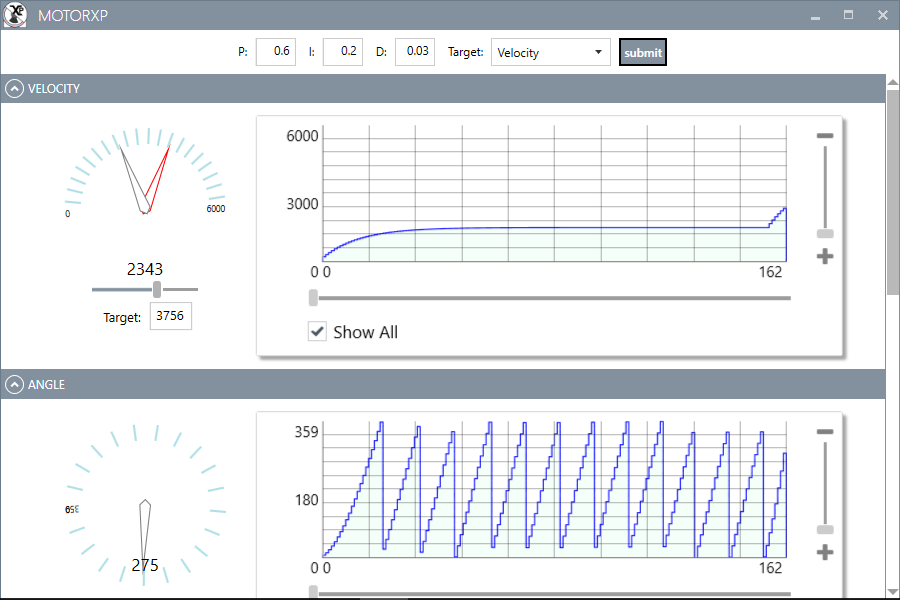
\includegraphics[width=.8\textwidth]{GUIScreenshot2}
		\caption{Ansicht der GUI zum Projektende}
		\label{fig:guifinal}
\end{figure}

Zum Abschluss der Implementierungsphase wurden Unit-Tests geschrieben, wodurch noch einige Fehler aus der Codebasis aufgespürt werden konnten. Diese Tests helfen ebenfalls zukünftigen Entwickler an dem Projekt, da unbedachte Änderungen welche zu Fehlverhalten der Applikation führen können schnell aufgedeckt werden.

\section{Ausblick}
Dieser Abschnitt beinhaltet mögliche Erweiterungen und nicht vollständig umgesetzte Projektteile, welche eine weitere Gruppe als Arbeitspaket aufnehmen kann. 

\begin{description}
\item[Multi-Plattformfähigkeit] Durch die Separierung der einzelnen Codeteile in eigenständige Projekte und die strikte Umsetzung eines Domain Driven Designs kann man die WPF GUI austauschbar machen und durch zum Beispiel eine Web-API ersetzen, welche anschließend mit einem Web-Frontend z.B. ASP.NET oder Angular2 kommuniziert. Auch eine Smartphone Applikation mit zum Beispiel Xamarin wäre möglich.
\item[MouseHover in LineChart] Diese Funktionalität konnte leider nicht Fertiggestellt werden, es wird noch nicht der aktuelle Wert unter der Maus angezeigt.
\item[Änderung des Layoutes] Durch eine Änderung des Layoutes wäre es möglich alle Sensorwerte auf einen Bildschirm Darzustellen, ohne die Notwendigkeit von Scrolbars zu haben. Empfehlung dafür wäre ein Wrappanel mit Horizontaler Ausrichtung.
\item[Hall Pattern Anzeige] Die Aktuelle Anzeige des Hall Pattern ist in einem extra Control unter dem ItemsTemplate für die Anzeigeelemente, dies verhindert Aktuell die einfache Umsetzung der vorher beschriebenen Änderung des Layouts. Hier müsste das Hall Pattern mit in das ItemsTemplate implementiert werden.
\item[ComPort Auswahl] Eine wichtige Erweiterung wäre eine Einstellmöglichkeit für den ComPort, da dieser aktuell Hardcoded ist und ggf. im Quelltext angepasst werden muss. Eine Notlösung wäre eine Auslagerung der Einstellung in eine Konfigurations-Datei. Aber die bessere Lösung wäre eine ComboBox in der GUI zur Auswahl aus verfügbaren Ports. 
\item[Mehrere Inputs] Die GUI könnte noch für mehrere Inputs erweitert werden um es zu ermöglichen mehrere Messstationen oder die Simulation nebeneinander Vergleichend laufen zu lassen.
\item[Benutzer Handbuch] Dem knappen Zeitrahmen geschuldet wurde noch kein Benutzerhandbuch erstellt. Dies wäre Sinnvoll nach der Änderung des Layouts zu erstellen, um aktuelle Bilder verwenden zu können.
\item[Weitere Tests] Sinnvoll für mehr Stabilität wären weitere Tests, einmal für die CustomControls (Gauge und LineChart) Unittests, für die Oberfläche allgemein Coded-UI Tests und ein automatisierter Integrationstest für das Kommunikationsmodul.
\item[Import/Export] Eine Im-/Exportfunktion um Testläufe zu sichern und wiederholt zu laden.
\item[RingSpeicher] Implementierung eines Ringspeichers, welcher eine Maximale Anzahl an Elementen fasst und überschüssige Daten auf der Festplatte oder ähnlich Speichert, um ein Überlaufen des Arbeitsspeichers zu verhindern.
\end{description}


%brauche folgende pakete
%\usepackage{tikz}
%\usetikzlibrary{circuits.ee.IEC}
%\usepackage{placeins}






\chapter{Arbeitspaket Simulation}
Für Analyse, Entwurf und Implementierung dieses Arbeitspakets übernahm Herr Welker die Verantwortung.


\section{Analysephase I - Verwendung existierender Bausteine}
Gemäß Projektspezifikation wurde gewünscht, dass die zu entwickelnde Simulation in Echtzeit laufen soll (1 Sekunde Simulation soll einer Sekunde in der Realität entsprechen), so dass die Simulationsergebnisse später ggf. mit dem realen Versuchsaufbau verglichen oder gar verbunden werden können. 

Zunächst wurde hierzu der Einsatz eines \textit{Rapid Prototyping System} von dSPACE erwogen. %https://de.mathworks.com/products/connections/product_detail/product_35337.html
Das Problem hierbei ist jedoch die Beschaffung (Hardware) und der nach bereits früher erhaltenen Aussagen extrem hohe Preis. 

Eine weitere Alternative wäre \textit{Simulink Desktop Real-Time}. %https://de.mathworks.com/products/simulink-desktop-real-time.html
Hier wird zwar keine kostspielige externe Hardware benötigt, aber auch die Anschaffungskosten von 2000 Euro %https://de.mathworks.com/pricing-licensing.html?prodcode=WT
wären für den Simulationsteil des Projekts wesentlich zu hoch. 

Aufgrund dieser Randbedingungen wurde von einer Simulation in Echtzeit zunächst wieder Abstand genommen.

Ein zusätzliches Ziel der Simulation sollte eine Kommunikations-Verbindung mit der GUI sein. Hierbei wäre es wünschenswert, wenn die Kommunikation äquivalent zur echten Hardware funktionieren würde, so dass mit ein- und derselben GUI sowohl Simulation als realer Versuchsaufbau angesprochen werden können. 

Da im realen Aufbau die Kommunikation zwischen $\mu$-Controller und PC mithilfe der seriellen Schnittstelle umgesetzt werden würde, sollte auch in der Simulation die Kommunikations-Verbindung mittels serieller Schnittstelle realisiert werden. 

Simulink stellt hierfür eigene Blöcke bereit, mit deren Hilfe es möglich ist, Modelle mit externen Geräten kommunizieren zu lassen.

Da in der Konzept-Phase nicht eindeutig ausgeschlossen werden konnte, dass Simulation und GUI ggf. auf demselben PC laufen würden, wurde eine Möglichkeit gesucht, dies mithilfe von virtuellen COM-Ports zu realisieren. 

Hierzu wurde das Programm \textit{Virtual Serial Port Driver} %http://www.eltima.com/de/products/vspdxp/ 
ausgewählt, mit dessen Hilfe es möglich ist, virtuelle COM-Ports zu erzeugen und diese virtuell zu verbinden. Damit wird es möglich, Simulation und GUI auf demselben PC laufen zu lassen und dieselben Schnittstellen zu verwenden wie bei Kommunikation mit externer realer Hardware.

Da die Simulation alle real verfügbaren Sensoren sowie das Verhalten des Motors möglichst gut abbilden soll, wurde weiterhin recherchiert, wie sich der reale Aufbau des Motor-Experimentierplatzes am besten in Simulink umsetzen ließ. Im Verlauf dieser Recherchen wurde festgestellt, dass es in Simulink bereits mehrere Modelle für einen solchen Aufbau (BLCD Motor mit Sensorik) gibt, die anhand ihrer Anpassbarkeit hinsichtlich der Motorparameter evaluiert wurden. 

Dabei stellte sich heraus, dass das Modell \textit{power\_pmmotor}
%https://www.facebook.com/l.php?u=https%3A%2F%2Fde.mathworks.com%2Fhelp%2Fphysmod%2Fsps%2Fexamples%2Fpermanent-magnet-synchronous-machine.html&h=2AQHLRXS auch als referenz verwendbar, wobei das Bild in matlab gemacht wurde
am besten hinsichtlich der Motorparameter eingestellt werden kann. 

Dieses Modell ist in Abbildung \ref{FigPowerPmmotor}
\begin{figure}[htbp]
	\centering
	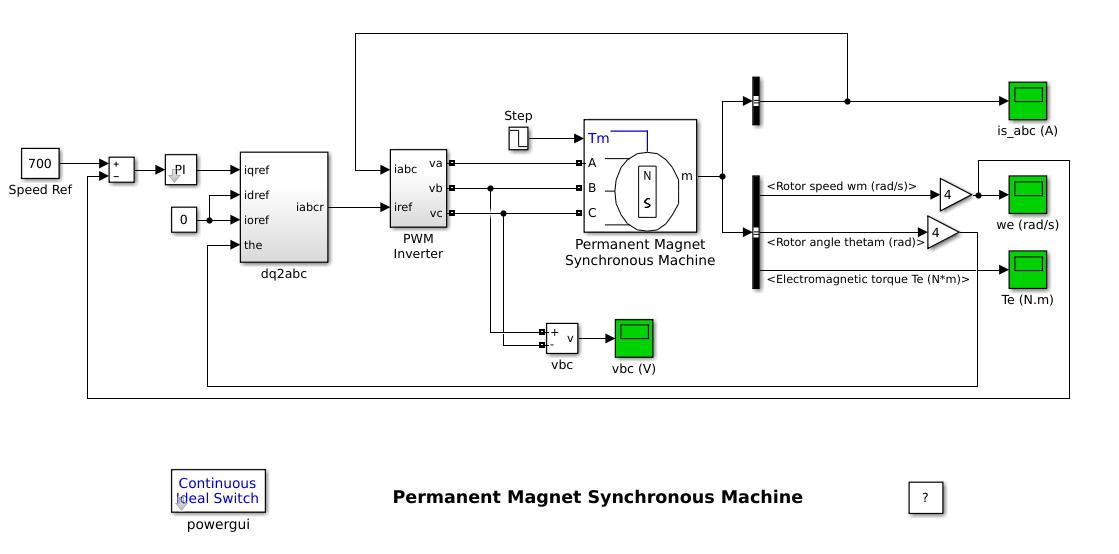
\includegraphics[width=0.8\textwidth]{./sim/pictures/powerPmmotor.png}
	\caption{power\_pmmotor Simulink Modell}
	\label{FigPowerPmmotor}
\end{figure}

zu sehen. Hier ist zu erkennen, dass in diesem Modell sowohl der Motor als auch die Sensorik (Hall-Sensoren) bereits umgesetzt sind. 

Das Modell bietet Einstellmöglichkeiten für folgende (in der Motorspezifikation angegebenen) Parameter des echten Motors sowie der Regelung:
\begin{itemize}
	\item Anzahl Polpaare
	\item Anzahl der Spulen
	\item Spulen Ansteuerungsform (sinusförmig)
	\item Rotor Typ (rund)
	\item Parameter für Modus (Generator- oder Motor-Betrieb)
	\item Spulen-Widerstand (0,33$\Omega$) 
	\item Drehmomentkonstante (0,065$Nm/A$)
	\item (Regelungsparameter): Motor-Regelung auf Drehzahl-Sollwert 
	\item P- und I-Anteil des Drehzahl-Reglers
\end{itemize}

Das Modell berechnet zusätzlich zur Drehzahl-Regelung das Motor-Drehmoment, die Werte der Hallsensoren sowie die Ströme in den Spulen. Des weiteren führt das Modell auch die Kommutierung durch, welche benötigt wird um das Drehmoment auf einem konstanten Level zu halten.

Im ersten Simulations-Modell wird also Simulink mit dem Modell \textit{power\_pmmotor} verwendet und per \textit{Virtual Serial Port Driver} an eine GUI angebunden (Implementierung des Kommunikations-Protokolls im Simulations-Kontext fehlt noch, der externe Kommunikationspartner wurde im Rahmen weiterer Teilgebiete dieses Projekts erstellt).


\section{Entwurfsphase und Implementierung I - Anpass-Arbeiten}
Es wurde damit begonnen, das Modell an den echten/geplanten Versuchsaufbau anzupassen:  
\begin{itemize}
	\item Um sich möglichst viele Freiheiten bei der Drehzahlregelung offen halten zu können, wurde geplant, einen PID-Regler zu verwenden. 
	\item Weiterhin wurden die zusätzlich benötigten Simulink-Blöcke für die serielle Kommunikation implementiert und passend parametrisiert. Da das Modell mit einem \textit{Solver} mit variabler Schrittgröße berechnet wird (hierbei berechnet der Lösungsalgorithmus von Simulink selbst, zu welchen Zeitpunkten die nächste Berechnung durchgeführt werden muss), konnte die Kommunikation nicht direkt umgesetzt werden, da die Kommunikationsblöcke nur mit \textit{Solvern} funktionieren die eine feste Schrittgröße (festes Abtastraster) verwenden. 
	Um dieses Problem zu lösen wurde hierfür ein \textit{Sample and Hold} Block eingesetzt. Dieser Block behält den Wert am Eingang so lange gültig, bis ein neuer Wert em Eingang anliegt, gibt am Ausgang jedoch zu definierten Zeiten einen Wert aus. Hiermit war es möglich zyklisch Daten aus dem Simulink Modell heraus zu senden und zu empfangen.
	\item Anschließend wurde äquivalent zum realen Versuchs-Aufbau begonnen Protobuff %todo: namen checken
	zu implementieren, da die GUI-Schnittstelle mit diesem Protokoll kommuniziert. Diese Arbeiten wurde dann zugunsten eines alternativen Motormodells (s.u.) allerdings auf Eis gelegt.
\end{itemize}


\section{Analysephase II - Alternativ-Modell}
Da ohne den echten Aufbau nicht weiter getestet werden konnte, ob das in der ersten Entwurfsphase ausgewählte Matlab Modell den Aufbau bereits ausreichend genau beschreiben kann und zum anderen die Komplexität dieses Modells sehr hoch ist, wurde beschlossen, ein neues, eigenes und nach Möglichkeit einfacheres Alternativ-Modell zu erstellen.


\section{Entwurfsphase II - eigene Motor-Modellierung}
Das Alternativ-Modell für den Motor sollte folgende Form haben - siehe Abbildung \ref{FigMotorBlock}:

\begin{figure}[htbp]
	\centering
	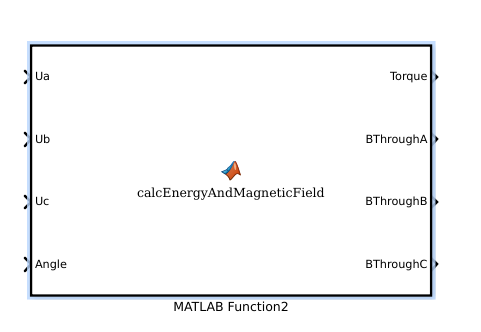
\includegraphics[width=0.6\textwidth]{./sim/pictures/matlabBox.png}
	\caption{Eigenschaften neuer Simulink Motor Block}
	\label{FigMotorBlock}
\end{figure}
Hierbei sind die Eingangsgrößen zu erkennen
\begin{itemize}
	\item $U_a$, $U_b$, $U_c$ an den drei Phasen U/V/W (an Spulen anliegende Spannung)
	\item Angle (Drehwinkel)
\end{itemize}
sowie die Ausgangsgrößen
\begin{itemize}
	\item \textit{BThroughA}, \textit{BThrougB} und \textit{BThrougC} (Spulen durchdringendes Magnetfeld)
	\item \textit{Torque} (Drehmoment)
\end{itemize}

\vspace{1cm}
Der Motor ist wie in Abbildung \ref{FigMotorAufbau} zu sehen ist aufgebaut:

\begin{figure}[htbp] 
	\centering
	\includestandalone{./sim/pictures/motorAufbau}
	\caption{Motor Aufbau}
	\label{FigMotorAufbau}
\end{figure}


Hierbei sind die 14 Permanentmagneten im außen laufenden Rotor zu erkennen. Diese sind so angeordnet, dass sich ihre Polung kontinuierlich abwechselt. 

Im Inneren des Motors sind die einzelnen Spulen des Stators zu erkennen. Mithilfe der farbigen Zuordnung ist es möglich zu identifizieren welche Spulen zu einer großen Spule (U,V oder W) zusammengeschlossen sind. 

Es ist zu erkennen, dass die großen Spulen sternförmig (über die Teil-Spulen 4, 5 und 12) zusammengeschaltet sind (der Sternpunkt des Motors ist von außen nicht zugänglich).
Die U/V/W-Anschlüsse sind mithilfe der Pfeile markiert (vgl. Spule 1, 8 und 9). 
Es sollte noch erwähnt werden, dass die Spulen unterschiedlich gewickelt sind. So sind die Spulen 1, 3, 6, 8, 9 und 11 im Uhrzeigersinn gewickelt und die Spulen 2, 4, 5, 7, 10 und 12 entgegen diesem.

In der symbolischen Abbildung ist zu erkennen, dass sowohl zwischen den Permanentmagneten im Rotor, als auch zwischen den Spulen im Stator jeweils Abstände existieren. 
Im realen Motor ist außerdem ein Luftspalt zwischen dem Rotor und dem Stator vorhanden. 
Die Formgebung der Polschuhe wird nicht dargestellt.


Vereinfachungs-Annahmen: 
Da ein einfaches Modell erstellt werden sollte, wurden folgende Annahmen getroffen, vgl. auch Abbildung \ref{FigVereinfachtesModell}:
\begin{itemize}
	\item Zwei der drei Phasen werden in der Darstellung mit Spannung versorgt, die dritte Spule ist offen.
	\item Alle Luftspalte werden vernachlässigt. D.h. weder die räumlichen Abstände zwischen den Permanentmagneten im Rotor noch der räumliche Verlauf der von den Spulen in Stator erzeugten Magnetfelder werden modelliert. 
	\item Weiterhin wird insbesondere auch der Luftspalt zwischen Rotor und Stator vernachlässigt.
	\item Es werden nur senkrechte Magnetfeldlinien angenommen, der Einfluss der Polschuhe wird vernachlässigt.
	\item Die Zuordnung der Spulen zu den großen Spulen, die Verbindung mit den Zuleitungen usw. entspricht der vorhergehenden Abbildung. 
\end{itemize}

\begin{figure}[htbp]
	\begin{center}
		\includestandalone{./sim/pictures/vereinfachtesModell}
		\caption{Vereinfachtes Modell}
		\label{FigVereinfachtesModell}
	\end{center}
	
\end{figure}


Um dieses Modell mithilfe von Arrays in Simulink umsetzen zu können, wurde gedanklich zwischen 1 und 12/14 aufgeschnitten und der Kreis ausgerollt. Dabei ergibt sich dann folgendes Bild \ref{FigAbgerolltesModell}.


\begin{figure}[htbp]
	\begin{center}
		\includestandalone{./sim/pictures/abgerolltesModell}
		\caption{Abgerolltes Modell}
		\label{FigAbgerolltesModell}
	\end{center}
	
\end{figure}

%\FloatBarrier
\section{Implementierung II - neues Motormodell}
Für die genaue Modellierung wurde folgender Ansatz verwendet: Sowohl für den Stator als auch den Rotor wird ein Array angelegt. Beim Rotor (Permanentmagnete) werden die Einträge mithilfe einer Konstanten für die magnetische Flussdichte gefüllt, dabei bekommt jeder Nordpol willkürlich gewählt ein positives und jeder Südpol ein negatives Vorzeichen. 

Da (wie im Bild zu erkennen ist) der Rotor 14 und der Stator zwölf Einheiten besitzen, wird die Anzahl der Arrayeinträge auf (mindestens) das kleinste gemeinsame Vielfache (84) festgelegt. Somit ist es mithilfe des Modells möglich den Motor simuliert in 84 Stufen zu drehen was einer Schrittgröße von ca. 4,3$^{\circ}$ entspricht. 

Für das Array des Stators wird berücksichtigt, welche Spulen aktuell bestromt sind und wie groß die angelegte Spannung ist. Mit Hilfe der Spannung und dem Spulen-Widerstand kann eine statische Stromstärke berechnet werden (die Induktivität der Spulen wird zunächst vernachlässigt), daraus lässt sich die magnetische Flussdichte in den Spulen bestimmen. 

Abhängig vom Winkel und der angelegten Spannung (d.h. welche Spulen bestromt sind) wird das Array für den Stator entsprechend befüllt. 

Anschließend wird abhängig vom Winkel das Rotor Array rotiert. 

Das resultierende Magnetfeld wird bestimmt, indem diejenigen Array-Einträge addiert werden, die sich einander gegenüber befinden. 
Die Einträge des so entstanden resultierenden Arrays werden quadriert (und durch die Konstante $2*\mu_0$ geteilt). 

Um am Ende die Energie zu errechnen, welche zu diesem Zeitpunkt im resultierenden Magnetfeld steckt, wird über die einzelnen Array-Einträge integriert. 
Somit ergibt sich ein Energiewert für diesen Zustand bzw. Zeitpunkt. 

Um das resultierende Drehmoment zu erhalten wird dieselbe Rechnung erneut durchgeführt, allerdings für den Fall, dass der Rotor $1/84$ weiter gedreht wird. 

Aus der Differenz dieser beiden Energiewerte kann das Drehmoment bestimmt werden unter der Annahme, dass die ganze Energie-Änderung in die Beschleunigung des Rotors eingeht.

Zusätzlich werden die resultierenden Magnetfelder über den Spulen (U,V und W) ebenfalls aufintegriert, um mit Hilfe dieser Werte im weiteren Modellaufbau die Induktionsspannung berechnen zu können.

\section{Bewertung des neuen Modells}
Bei der Untersuchung des neuen Modells muss festgehalten werden, dass die Induktivität der Spulen nicht mithilfe dieses Modells berechnet werden kann. 
Der modellierte Magnetfeld-Verlauf für eine Spule hat die in Abbildung \ref{FigResultierendesFeld}
dargestellte Form.

\begin{figure}[htbp]
	\centering
	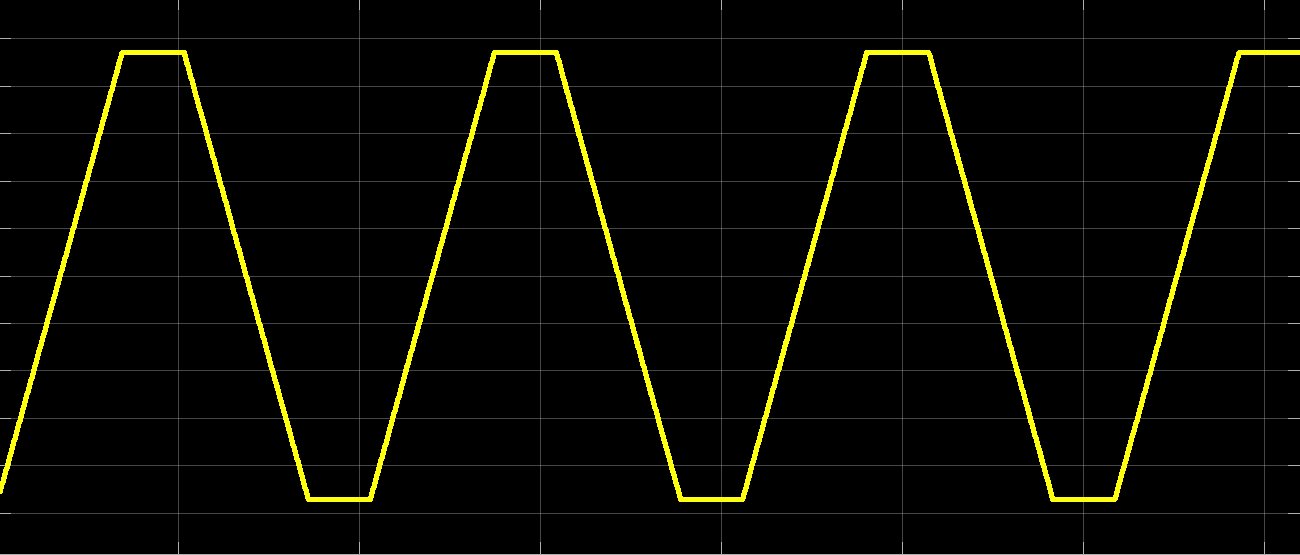
\includegraphics[width=0.8\textwidth]{./sim/pictures/resultierendesFeld.png}
	\caption{Verlauf Magnetfeld in einer Spule}
	\label{FigResultierendesFeld}
\end{figure}

Dies lässt sich dadurch begründen, dass bei der Betrachtung einer Spule (z.B. der V-Spule) für das Feld im Stator 4*7= 28 Array-Elemente des resultierenden Arrays beteiligt sind. Über diese wird integriert, um die Größe für das Feld zu bekommen, was einer Aufsummierung der beteiligten Array-Elemente entspricht $\sum \limits_1^{28} V_{res_i}$. 

Wobei sich ein Eintrag $V_{res_i}$ aus der Addition des Spuleneintrags $V_i$ und des Eintrags des darüber liegenden $R_i$ also dem Wert des Rotormagnetfeldes an dieser Stelle ergibt. So lässt sich $\sum \limits_1^{28} V_{res_i}$ zu $\sum \limits_1^{28} (V_i+R_i)$ umstellen. Diese Summe lässt sich nun allerdings nun in zwei Summen zerlegen, zum einen in $\sum \limits_1^{28} V_i$ und zum anderen $\sum \limits_1^{28} R_i$. 

Hierbei ist die erste Summe  $\sum \limits_1^{28} V_i$ immer 0, da die vier Spulen einer großen Spule (im Beispiel Phase V) in der Wicklungsrichtung abwechseln. 

Somit bleibt nur noch $\sum \limits_1^{28} R_i$ übrig um den Verlauf zu erklären: Wie in Abbildung \ref{FigAbgerolltesModell} zu erkennen ist, ist ein Element des Rotors kleiner als eines des Stators. So kürzen sich zwar auch viele Elemente des Rotors heraus, jedoch nicht alle. Dies führt zum erkennbaren Magnetfeld-Verlauf. 

Das hat jedoch nicht wirklich etwas mit dem Verlauf zu tun, der modelliert werden soll. Aus diesem Grund ist das Modell hierfür nicht passend und sollte nicht ohne weitere Änderungen verwendet werden (insbesondere bedeutet eine ausschließlich statische Betrachtung der Magnetfeldverläufe eine unzulässige Vereinfachung).

Hingegen scheint der Verlauf für das Drehmoment durchaus Sinn zu ergeben, wie in Abbildung \ref{FigDrehmoment} zu erkennen ist: Da in diesem Modell in die Berechnung der resultierenden  Energie ein Quadrat eingeht, ist hier das zuvor beschriebene Verhalten des Wegkürzens nicht mehr vorhanden. 

Es ist jedoch noch darauf hinzuweisen, dass eine Vergrößerung der Anzahl an Array-Elementen (entspricht einer Erhöhung der Auflösung) nicht dazu führt, dass dieser Verlauf glatter werden würde, sondern es werden immer dieselben zwölf Stufen, welche den Spulen-Polpaaren entsprechen, im Verlauf zu erkennen sein.
Dies ist eine Folge der zu Beginn getroffenen Vereinfachungen, wonach Luftspalt, Polform und nicht-senkrechte Magnetfeldlinien vernachlässigt wurden.


\begin{figure}[htbp]
	\centering
	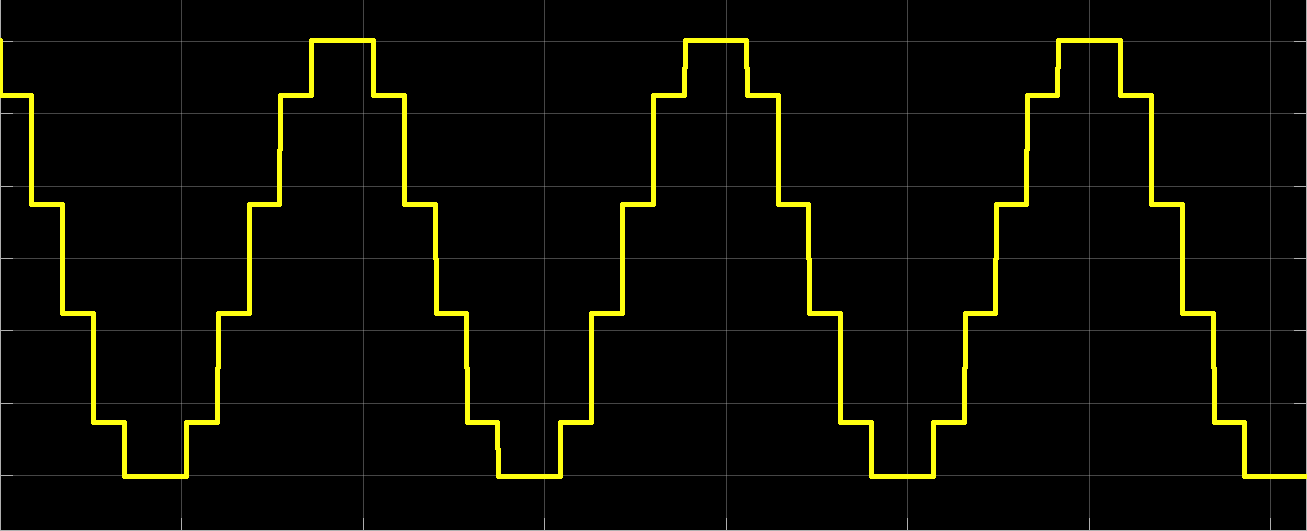
\includegraphics[width=0.8\textwidth]{./sim/pictures/drehmoment.png}
	\caption{Drehmoment bei Spannung an $U_a$ und Masse bei $U_b$}
	\label{FigDrehmoment}
\end{figure}


\section{Bewertung der beiden Modelle}
Für eine Simulation des Motor-Experimentierplatzes ist das zweite Modell (zumindest in der vorliegenden Form) nicht geeignet, es geht von statischen Zuständen aus und vernachlässigt die dominanten Parameter (Induktivität, Luftspaltgestaltung usw.) eines realen Motors.

Ein Vergleich des ersten Modells mit dem Verhalten des realen Experimentierplatzes steht noch aus.

\section{Ausblick}
Für das neue, zweite Modell gibt es noch viel Verbesserungs-Potenzial, z.B.:

\begin{itemize}
	\item So wäre es möglich, bzw. wurde schon damit begonnen, die Kommutierung umzusetzen. Diese soll anhand des Winkels die Spulen unterschiedlich an Masse und Spannung anschließen mit dem Ziel ein konstantes Drehmoment zu erhalten.
	
	\item Mit dieser Erweiterung könnte dann ein (Strom-/Drehmoment-)Regler implementiert werden welcher z.B. auf ein konstantes Drehmoment regelt.
	
	\item Das reale Drehmoment ist eine Funktion zahlreicher mechanischer und elektromagnetischer Details der Motorgestaltung. Einfluss der Induktivität, Luftspaltgestaltung usw. könnten Gegenstand weiterer Modell-Verfeinerungen sein. 
	
	\item Um das neue Modell in die Simulationsumgebung anstelle des ersten Modells einbetten zu können, sind dieselben Erweiterungen durchzuführen, mit denen bereits am ursprünglichen Modell begonnen wurde (z.B. damit auch dieses Modell in der Lage wäre mit der GUI zu kommunizieren, um simulierte Größen auszutauschen bzw. von dort Regelgrößen zu bekommen).
\end{itemize}

Zuvor sollte das erste Modell (Matlab-Bausteine) weiter mit dem Verhalten des realen Motor-Experimentierplatzes verglichen werden (Messwerte). 

Da der reale Aufbau noch nicht fertiggestellt war, konnte hierfür noch keine eindeutige Modell-Bewertung gegeben werden.





\chapterauthor{Christian Brunner}

\newcommand{\quelle}{%
	\small Quelle:
}

\newcommand{\registered}{\textsuperscript{\textregistered}}

%Einzug bei neuem Absatz auf 0pt Einrücken
%\setlength{\parindent}{0pt}

\chapter{Hardware}


Im Rahmen des Projektes wurden unterschiedlichste Komponenten von verschiedenen Herstellern eingesetzt.
Dieses Kapitel soll einen Überblick über die verwendete Hardware geben.
Darunter einige Eigenschaften und Besonderheiten auf die ggf. in den Nachfolgenden Unterabschnitten näher eingegangen wird.

%----------------------------------------------------------------------------------
\section{Infineon XMC 4700/4800 Relax Kit}
\label{sec:INF XM4700/4800}
Für die Auswertung der verschiedenen Sensoren wurden Mikrocontroller des Herstellers Infineon aus der XMC 4000 Serie genutzt.
Diese werden kurz beschrieben.
Im Anschluss wird auf Probleme mit diesen eingegangen.

\subsection{Allgemeine Beschreibung} 
\paragraph{Hinweis:} Da die Mikrocontroller XMC 4700 und XMC 4800 nahezu identisch sind ist die nachfolgende Beschreibung für beide Controller gültig.
Auch wird zwischen den beiden Relax Kits nicht unterschieden
Auf die Besonderheiten nach dem folgenden Abschnitt eingegangen.

\paragraph{XMC Mikrocontroller:}
Bei dem XMC Relax Kit handelt es sich um eine Entwicklungsplattform für den XMC Mikrocontroller.
Innerhalb des Controllers arbeitet ein ARM\registered Cortex\registered-M4 mit einer Taktfrequenz von 144 MHz.
Dieser bildet die CPU, welche um zahlreiche Schnittstellen erweitert wird.
Als Kommunikationsschnittstellen stehen unter anderem Ethernet, USB,  CAN und USART zur Verfügung.
Für die Erfassung Analogen Signalen stehen mehrere \enquote{Versatile Analog-Digital Converters} (VADC) mit je 8 Kanälen und einer Auflösung von 12-Bit zur Verfügung.
Weiterhin sind Digital-Analog-Konverter(DAC) mit einer Auflösung von 12-Bit integriert.

Eine Besonderheit der XMC 4000 Serie ist das \enquote{Position Interface} (POSIF).
Dieses Modul stellt eine Schnittstelle für die Steuerung von Motoren bereit.
Hierzu kann POSIF wahlweise mit Hall-Sensoren, Drehgebern oder mittels Software versorgt werden.
Aus diesen Sensorinformationen wird im Anschluss ein Steuersignal für die Ansteuerung des Motors generiert.\cite{InfineonTechnologies2016a}
%Hierbei handelt es sich um ein Modul für die Steuerung von verschiedensten Motoren unter Verwendung von Hall-Sensoren, Drehgebern oder externen Steuersignalen. \cite[Kap. 25]{InfineonTechnologies2016}
%ref Reference Manual Chap 25.2.7.1

Eine vollständige Auflistung der enthaltenen Komponenten kann dem Referenzhandbuch \cite{InfineonTechnologies2016} oder der Produkthomepage \cite{InfineonTechnologies2017} entnommen werden .

\newpage
\paragraph{Relax Kits:}
Infineon stellt, für die Einarbeitung und Tests, kleine Entwicklungsplattformen bereit.
Dabei handelt es sich um Platinen, die bereits mit einem XMC Mikrocontroller und allen dafür notwendigen Bauteilen versehen ist.
Zum Teil sind diese Entwicklungsplatinen für die Aufnahme von sog. Arduino Shields vorgesehen um Modular den Mikrocontroller zu erweitern.
Hier ist jedoch zu beachten, dass nicht jedes Relax Kit alle Erweiterungsplatinen aufnehmen kann.
Für das Aufspielen von Programmen bzw. zum Debuggen verfügen die Relax Kits über eine JTAG Schnittstelle\footnote{Kurzform für Joint Test Action Group und Synonym für IEEE-Standard 1149.1.}.

In Abbildung \ref{fig:XMC4700} ist Beispielhaft eines der Relax Kits dargestellt, die während des Projektes zum Einsatz kamen.
In der Mitte befindet sich der Mikrocontroller. 
Über- und Unterhalb von diesem sind Buchsenleisten für die Aufnahme von Arduino Shields bereits aufgelötet.
Die noch nicht bestückten Lötaugen sind mit dem Controller verbunden und können mit Stift- oder Buchsenleisten versehen werden.
In der linken unteren Ecke ist die JTAG Schnittstelle angebracht, die mittels eines Micor-USB Anschlusses mit einem PC verbunden werden kann. 

\subsection{XMC 4700 Relax Kit 5V}
\label{sec:XMC4700}
Dieses Kit ist für die Verwendung der Arduino Shields vorgesehen.
Da es sich bei der Arduino Plattform um 5 Volt Mikrocontroller handelt sind die Shield vorwiegend auf diese Spannung ausgelegt.
Der XMC arbeitet hingegen mit einem Logikpegel von 3.3 Volt.
Aus diesem Grund hat Infineon für die Digitalen Pins Bidirektionalen Levelshifter verbaut.
Mit diesen werden die 5 Volt Signal auf 3.3 Volt bzw. anderes herum gewandelt.
Dadurch kann eine Vielzahl von Erweiterungsplatinen ohne Änderungen verwendet werden.

\begin{figure}[h]
	\centering
	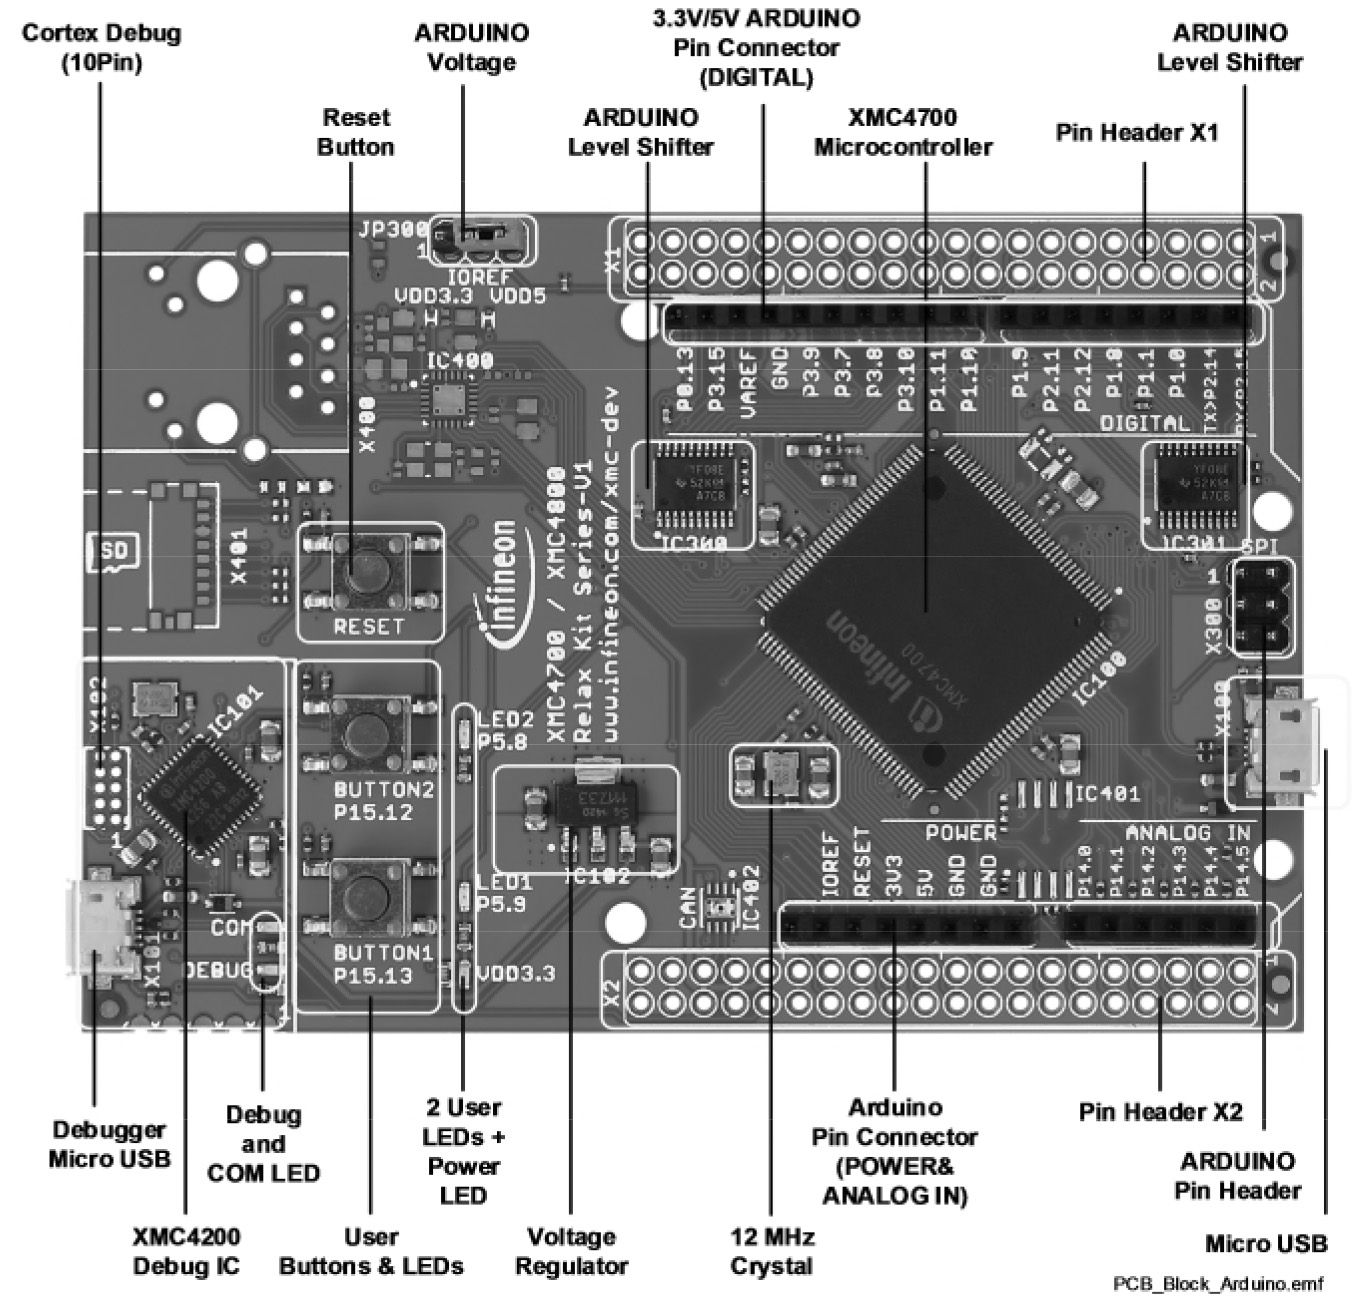
\includegraphics[width=\textwidth-6cm]{hardware/graphics/XMC_4700_Board_overview}
	\caption{XMC 4700 Relax Kit 5V}
	\quelle \url{http://www.infineon.com}
	%quelle http://www.infineon.com/export/sites/default/media/products/Microcontrollers/XMC/XMC4700_Relax_Kit.JPG_472149771.jpg
	\label{fig:XMC4700}	
\end{figure}

\paragraph{Bidirektionale Spannungswandler TXS0108:}
Auf dem Relax Kit sind für die Pegelwandlung von 5 Volt zu 3.3 Volt zwei Levelshifter vom Typ TXS0108 aufgebracht.
Diese setzen einen angelegten Logischen Pegel von einer Quellspannung auf eine zweite um.
Dies kann bidirektional geschehen.
Dadurch ist es möglich die I/O Pins als Ein- oder Ausgang zu verwenden.

Ein Problem, dass während der Durchführung des Projektes auftrat war ein Schwingen bzw. ein Burst-Signal. 
Ursache hierfür waren zu lange Anschlussleitungen.
Der Hersteller, Texas Instruments, verweist in seinem Handbuch darauf, dass die Leitungslänge kurz gehalten werden muss um Reflexionen zu vermeiden.
Das Verhalten bei solchen Reflexionen wird nicht näher beschrieben.
Genaueres kann dem Abschnitt Hardwaretest und Analyse entnommen werden.
Unter Normalbedingungen, damit ist die Verwendung der Levelshifter mit Arduino Shields gemeint, dürfte ein solches Problem nicht auftreten, da die Signalleitungen nur wenige Zentimeter betragen.

%----------------------------------------------------------------------------------


\subsection{XMC 4800 Relax EtherCat Kit}
\label{sec:XMC4800}
Dieses Kit entspricht, mit ein paar Unterschieden, dem XMC 4700 Relax Kit 5V.
Auf diesem Kit befinden sich keine Levelshifter.
Dies sind durch 0-Ohm Widerstände ersetzt.
In Abbildung \ref{fig:XMC4800} sind diese entsprechend markiert.
Dadurch ist die Verwendung von 5 Volt Arduino Shields nicht möglich.
Des weiteren ist bereits eine Anschlussbuchse für Ethernet und ein EtherCat Adapterboard vorhanden.
Bei EtherCat handelt es sich um eine echtzeitfähige Ethernet Kommunikation, die vorwiegend in der Automatisierungstechnik eingesetzt wird. 

\begin{figure}[hptb]
	\centering
	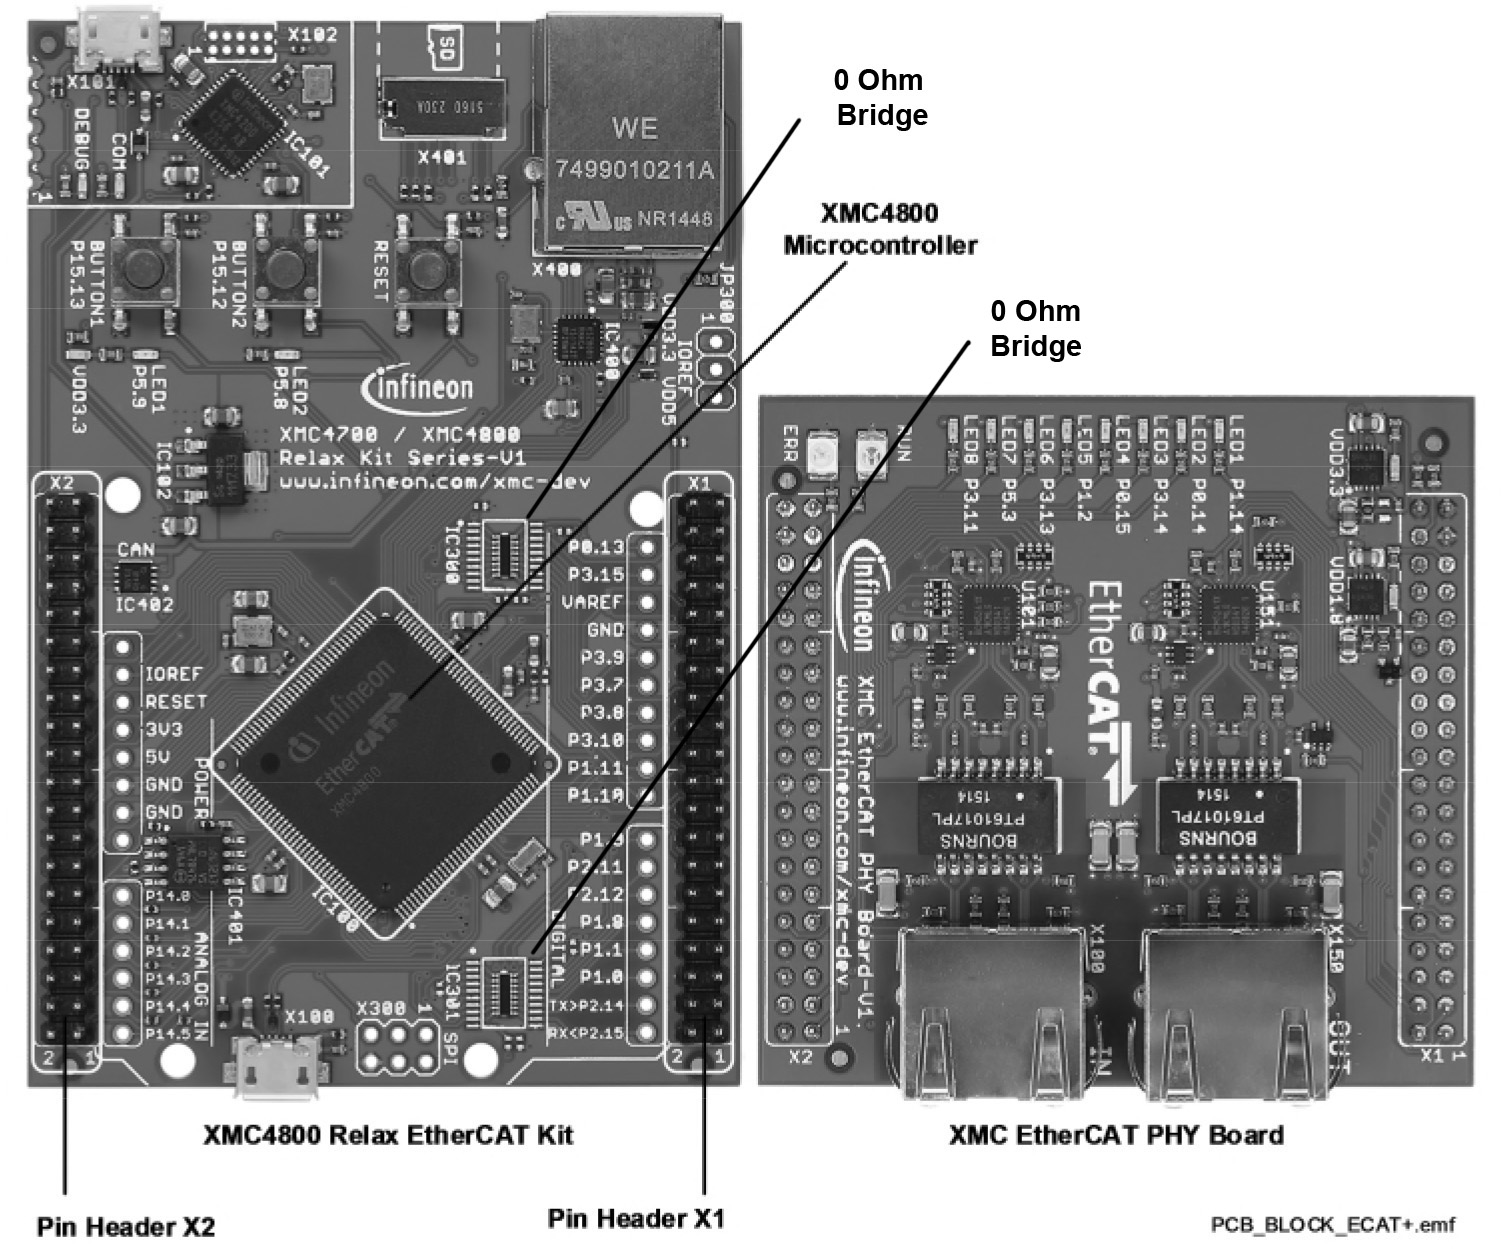
\includegraphics[width=\textwidth-4cm]{hardware/graphics/XMC_4800_Board_with_EtherCAT}
	\caption{XMC 4800 Relax Kit mit EtherCat PHY Board}
	\quelle http://www.infineon.com
	%quelle 
	\label{fig:XMC4800}
\end{figure}

%----------------------------------------------------------------------------------

\newpage
\section{Texas Instrument DRV8302 Evaluation Kit}	
\label{sec:TI DRV8302 EvalKit}
Mit diesem Kit stellt Texas Instrument eine fertig Plattform für die Entwicklung von Motorsteuerungen und das Experimentieren mit BLDC-Motoren\footnote{BLDC ist die Kurzform für Brushless DC und bezeichnet den Grundlegenden Aufbau eines Motors.} zur Verfügung.
Es besteht aus dem Evaluation Board, Controller Karte, Anschlusskabeln und einer Steuerungssoftware für die Controller Karte (siehe Abbildung \ref{fig:DRV8302EvalKit}).
Damit ist es ohne großen Aufwand möglich BLDC-Motoren anzusteuern.
Über verschiedene, auf der Platine vorhandenen, Schutzmechanismen wie Überstrombegrenzung soll ein Zerstören des Angeschlossenen Motors verhindert werden.

\begin{figure}[h]
	\centering
	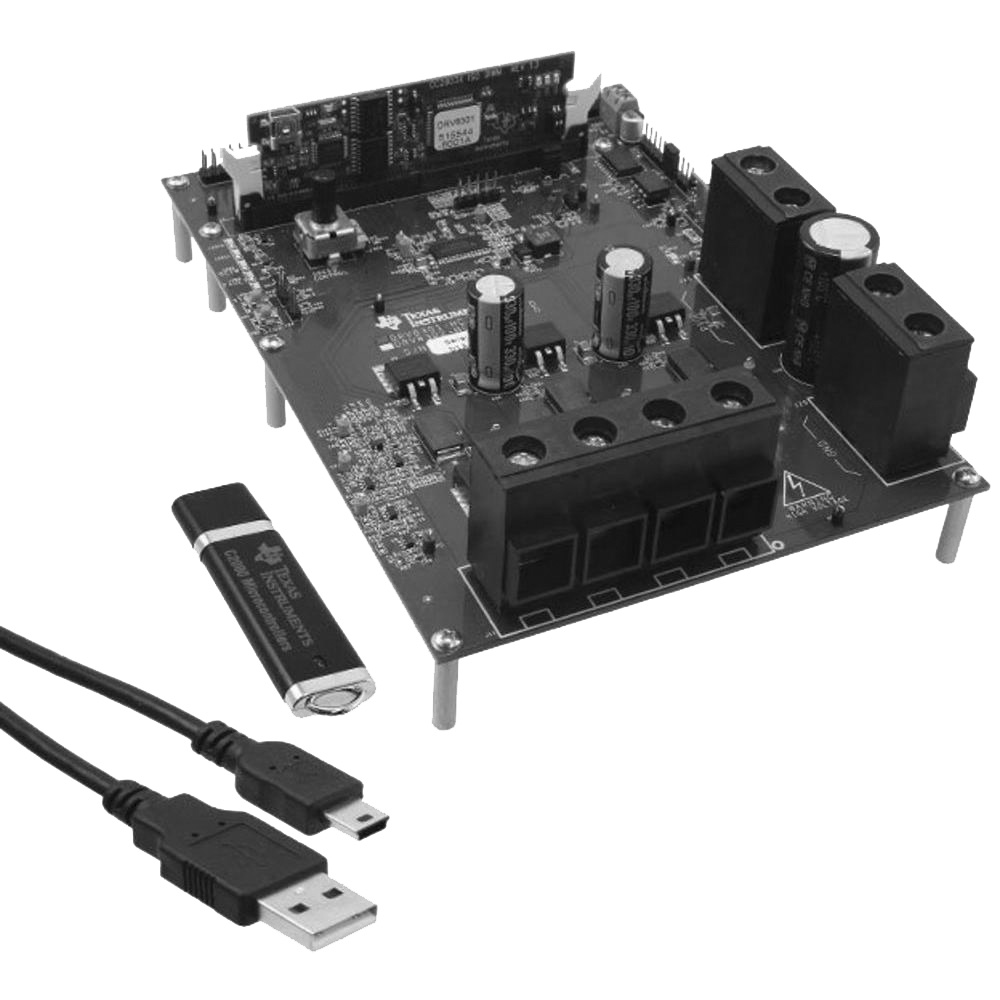
\includegraphics[width=8cm]{hardware/graphics/1189086_BB_00_FB}
	\caption[DRV8302 Evaluation Kit]{Texas Instrument DRV8302 Evaluation Kit}
	\quelle http://www.ti.com
	\label{fig:DRV8302EvalKit}
\end{figure}

In Abbildung \ref{fig:DRV8302Board} ist das Evaluation Board dargestellt.
Kernstück des Evaluation Boards ist ein Drei-Phasen-Treiberchip (DRV8302).
Dieser steuert die darunter liegenden Feldeffekttransistor, welche den Arbeitsstrom auf die verschiedenen Wicklungen des Motors schalten.
Der DRV8302 kann mit einer Spannung von 8 V bis 60 V Gleichspannung versorgt werden.
Die Leistungstransistoren können eine Spitzenstrom von 60 A pro Phase schalten.
Am unteren Ende der Platine befindet sich das Anschlussterminal für den Motor.
Rechts daneben das für die Versorgungsspannung.\\

\begin{figure}[htbp]
	\centering
	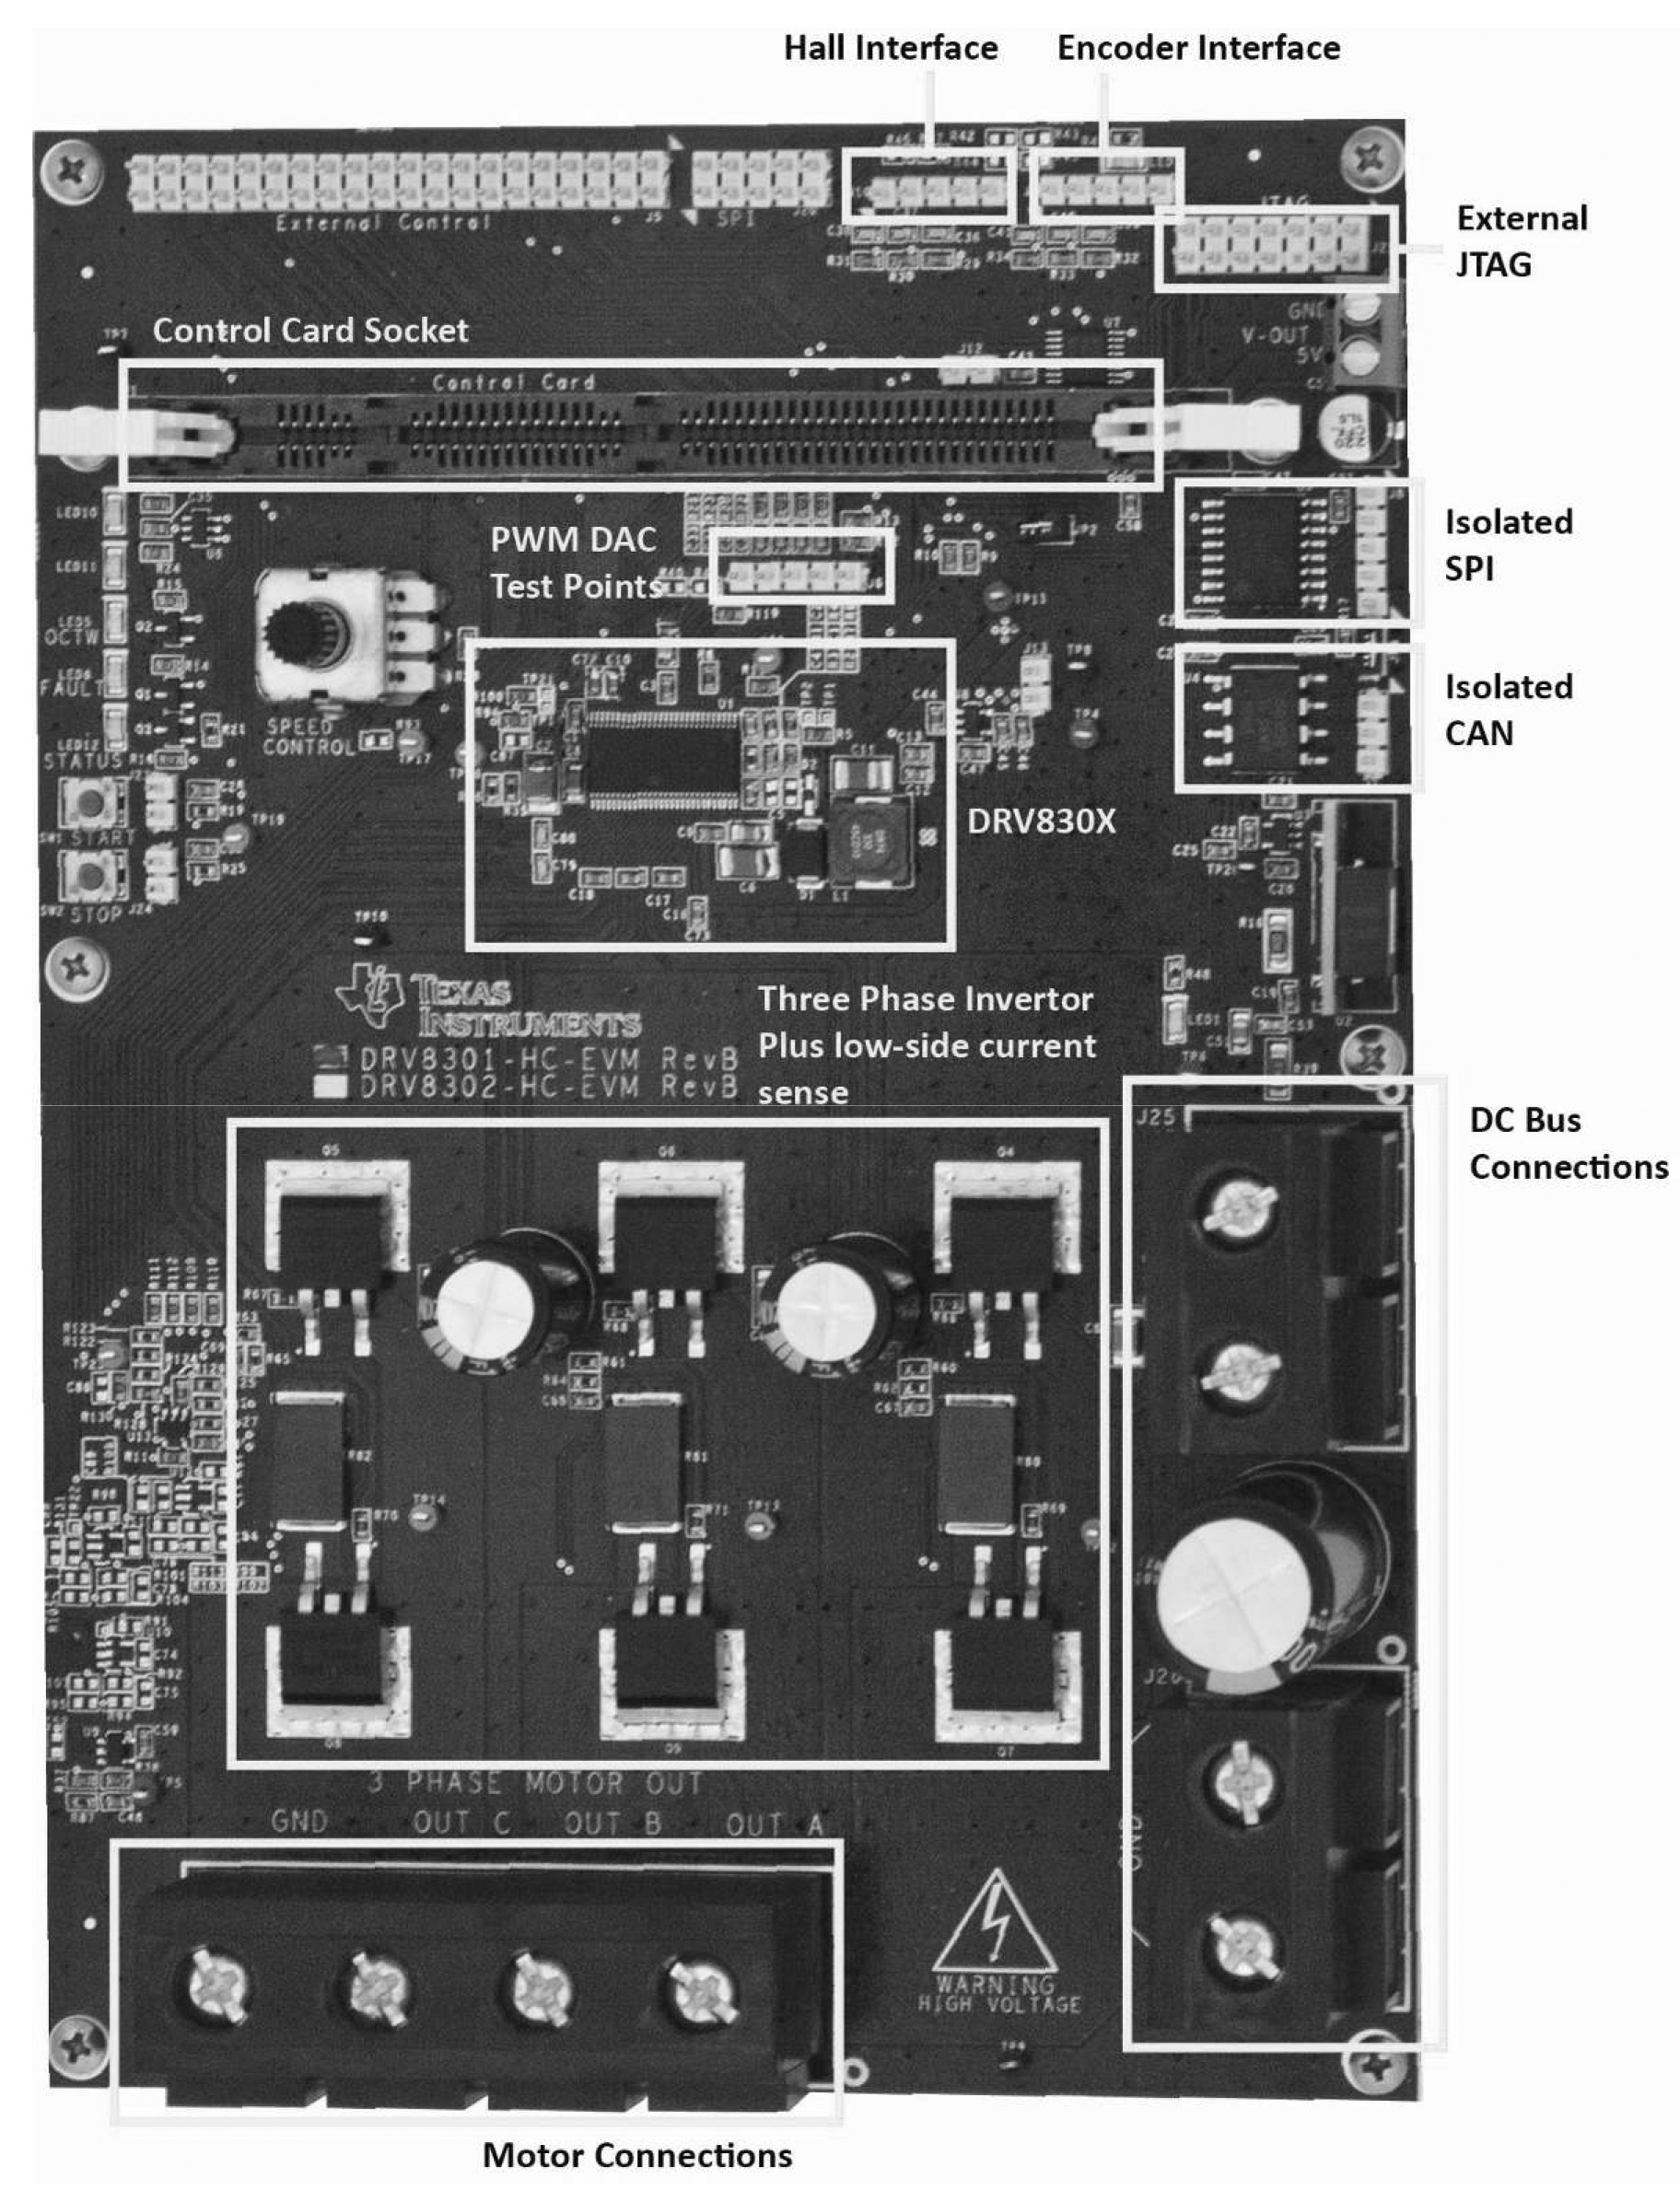
\includegraphics[width=\textwidth]{hardware/graphics/TI_Eval_Board}
	\caption{DRV8302 Evaluation Board}
	\quelle \cite{Instruments2014}
	\label{fig:DRV8302Board}
\end{figure}

Zur Ansteuerung der Leistungstransistoren werden mehrere Steuersignale benötigt.
Diese erzeugt der Treiberchip, welcher seine Signale von einem externen Controller erhält.
Der DRV8302 kann dazu in zwei unterschiedlichen Betriebsmodi betrieben werden.
Entweder alle sechs Steuersignale für die Leistungstransistoren stellt der externe Controller bereit oder es werden nur drei Signale bereitgestellt.
Der erste Fall (6 Steuersignale) gibt dem Nutzer bzw. dem externen Controller die Möglichkeit beide MOSFETs auf LOW zu schalten.
Dadurch wird erreicht dass nur zwei Motorleitungen (z.B. U und W) einen geschlossenen Stromkreis bilden und nur über diese beiden Spulen Strom fliest.
Im Gegensatz dazu ist es im zweiten Fall (3 Steuerleitungen) nur möglich eine Motoranschlussleitung auf HIGH oder LOW zu legen. 
Es müssen also alle drei Leitungen für die Generierung des Motorsignals herangezogen werden.
%todo weiterschreiben. Auch noch ein Beispiel bringen
%----------------------------------------------------------------------------------

\newpage
\section{PMD-BLDC-1500/65}
Als Motor für den Experimentierplatz wird ein Bürstenloser Gleichstrommotor eingesetzt (kurz BLDC), genauer gesagt ein LRK Motor. 
Benannt ist dieser nach den drei Person, die an seiner Entwicklung beteiligt waren.
Christian \textbf{L}ukas hatte Ende 2000 die Idee von diesen Motoren, die Ludwig \textbf{R}etzbach in der Elektro-Modell veröffentlichte, und Herr \textbf{K}ühfuß die ersten Drehteile herstellte.
%quelle http://www.torquemax.de/Motoren/default.html
Es handelt sich dabei um einen sog. Außenläufer.
Bei diesem bildet die Motorabdeckung, in der sich 14 Magnete befinden, den Rotor.
Die Motorwicklung im Inneren ist starr und mit Kupferdraht umwickelt.\\


Der allgemeine Vorteil von Bürstenlosen Motoren liegt darin, dass es keine Verschleißteile gibt.
Hingegen müssen bei klassischen Gleichstrommotoren mit Bürsten diese ersetzt werden sobald sie verbraucht oder zerstört sind.
Zur Regelung des BLDC-Motors sind drei digitale Hall-Sensoren verbaut.
Diese Sensoren reagieren auf Magnetfelder und ändern bei einem bestimmten Schwellwert ihren Ausgangspegel.
Genaueres ist dem Abschnitt Sensor zu entnehmen.\\


Zur Temperaturüberwachung ist ein NTC-Sensor innerhalb des Motors angebracht. 
NTC ist hierbei die Kurzform für Negative Temperature Coefficient Thermistor und beschreibt einen Temperaturabhängigen Widerstand.
Dieser verringert seinen Widerstand bei steigender Temperatur.\\

In Abbildung \ref{fig:BLDC} sieht man den Motor mit den drei Motoranschlussleitungen.
Der daneben liegende Stecker mit sieben weiteren Kabeln ist das Anschlussterminal für die Hall-Sensoren und den Temperatursensor.
Auf der Vorderseite ist die Welle und darum die Befestigungslöcher zu sehen.

\begin{figure}[htbp]
	\centering
	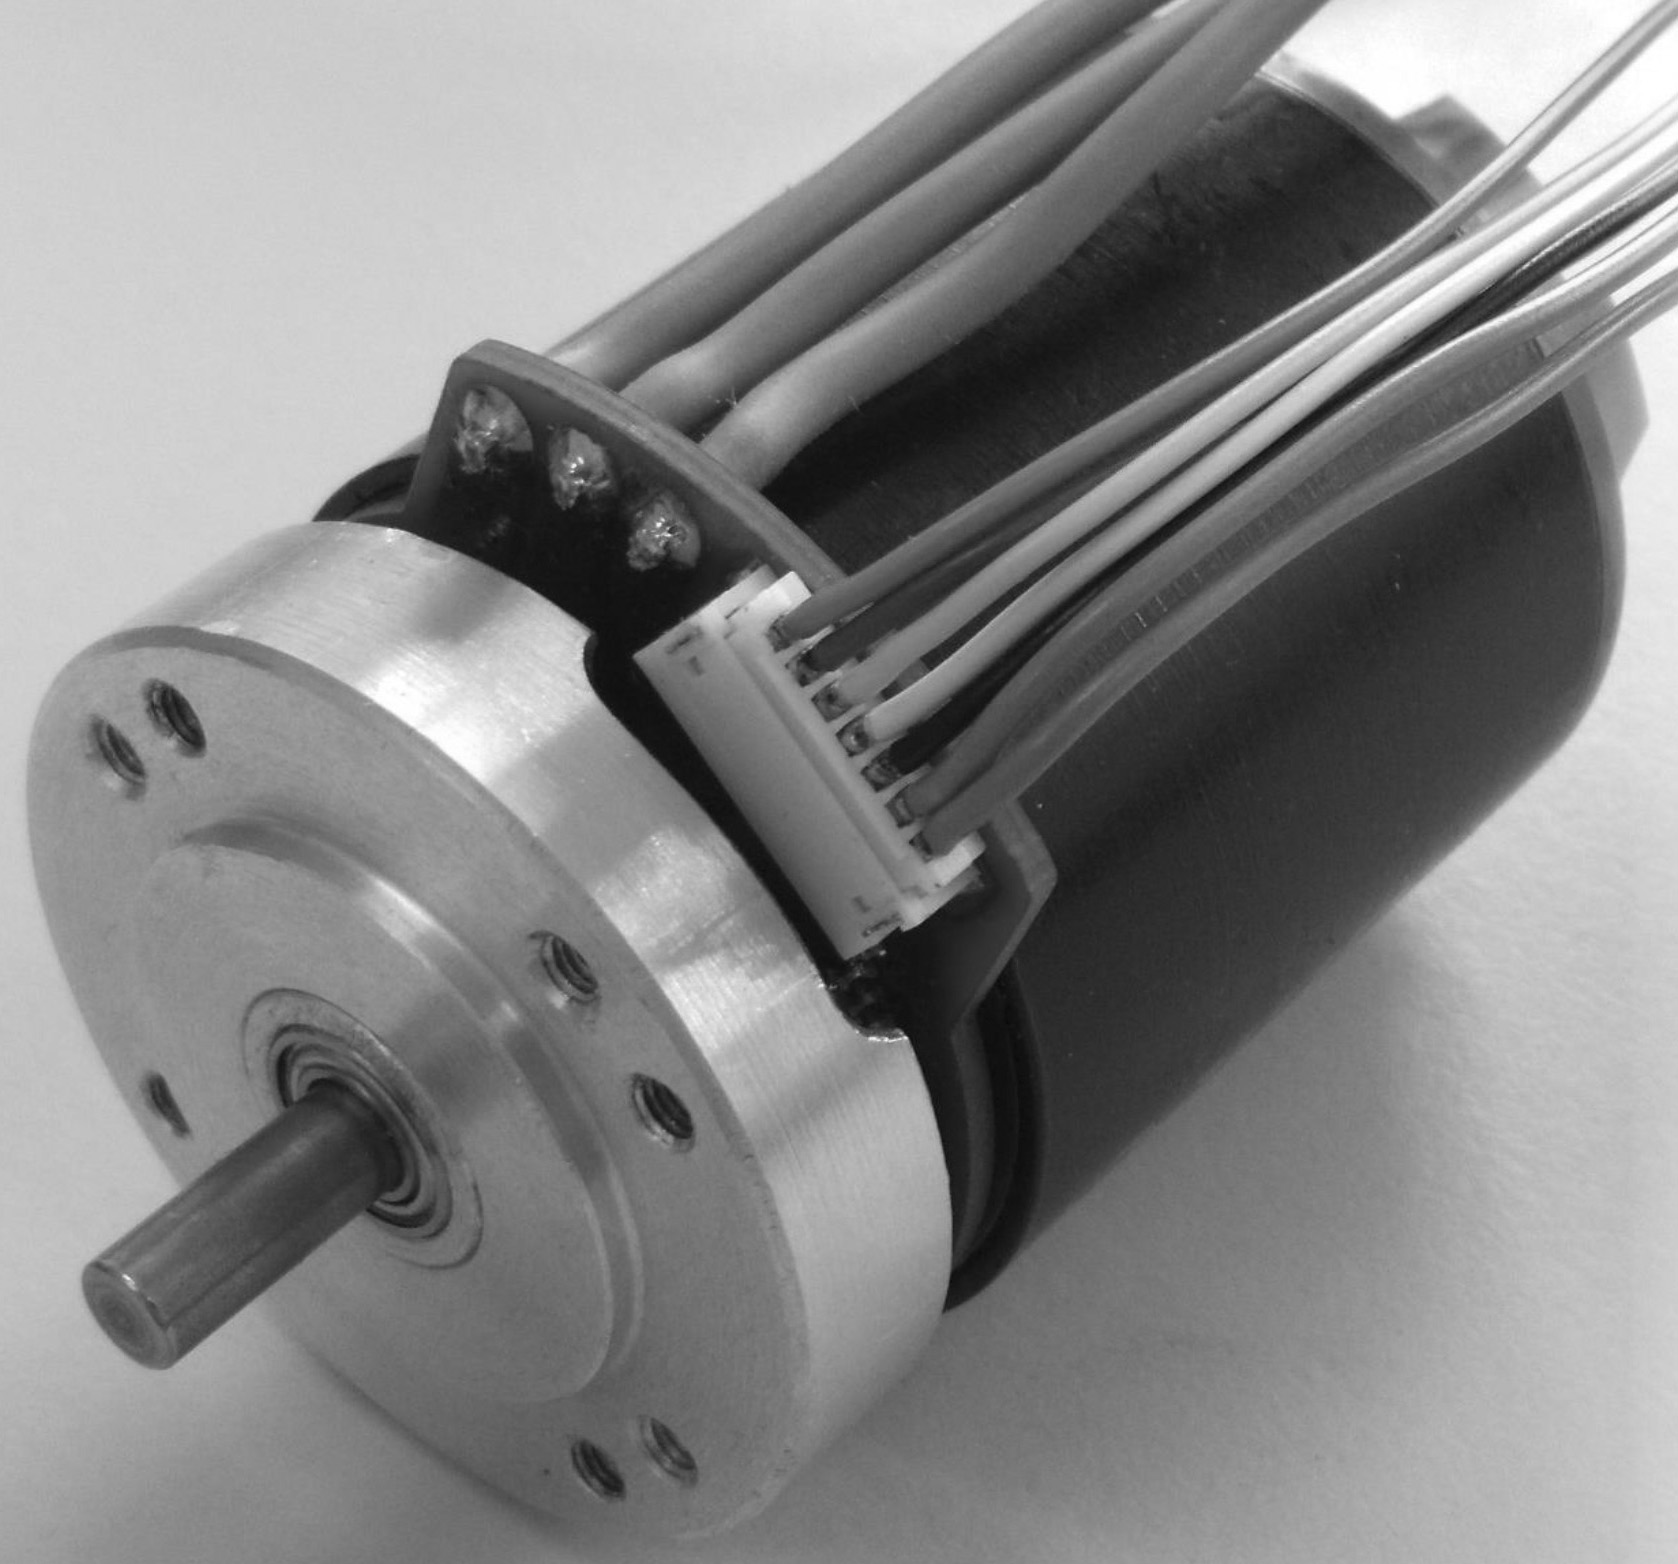
\includegraphics[width=6cm]{hardware/graphics/BLDC_Motor}
	\caption{PMD-BLDC-1500/65 Motor}
	\quelle Herstellerdatenblatt
	\label{fig:BLDC}
\end{figure}

\newpage
\section{BLDC Motorprüfstand}
Bei dem Prüfstand handelt es sich um eine Grundplatte aus Holz mit den ungefähren Abmessungen von 60 cm mal 40 cm.
Auf dieser sind Aluminiumprofile montiert, die das Grundgerüst für verschiedene Halter bilden.
Über die Profile ist es recht einfach möglich, den gesamten Aufbau zu verschieben.\\


Die verschiedenen Hardwarekomponenten bilden zusammen den Motorprüfstand.
In Abbildung \ref{fig:Schemata_Hardware_Gesamt} ist dies schematisch dargestellt.
Der BLDC-Motor wird über die H-Brücke bzw. dem Texas Instrument DRV8302 Evaluation Kit gesteuert.
Dieses erhält seine Steuersignale wiederum von einem Mikrocontroller. 
In der Abschlusskonfiguration war dies das XMC 4800 Relax EtherCat Kit.
Um Fehler detektieren zu können werden Sensorsignale von der H-Brücke und BLDC-Motor an den Mikrocontroller gesendet.
Der Controller selbst bildet in Verbindung mit den Sensorsignalen einen Regler.
Dessen Parameter erhält er von einer PC Applikation an die auch die Sensorwerte weitergeleitet werden.
Dort werden diese grafisch aufbereitet und in verschiedenen Diagrammen dargestellt.

%todo noch etwas über den Motorprüfstand schreiben

\begin{figure}[htbp]
	\centering
	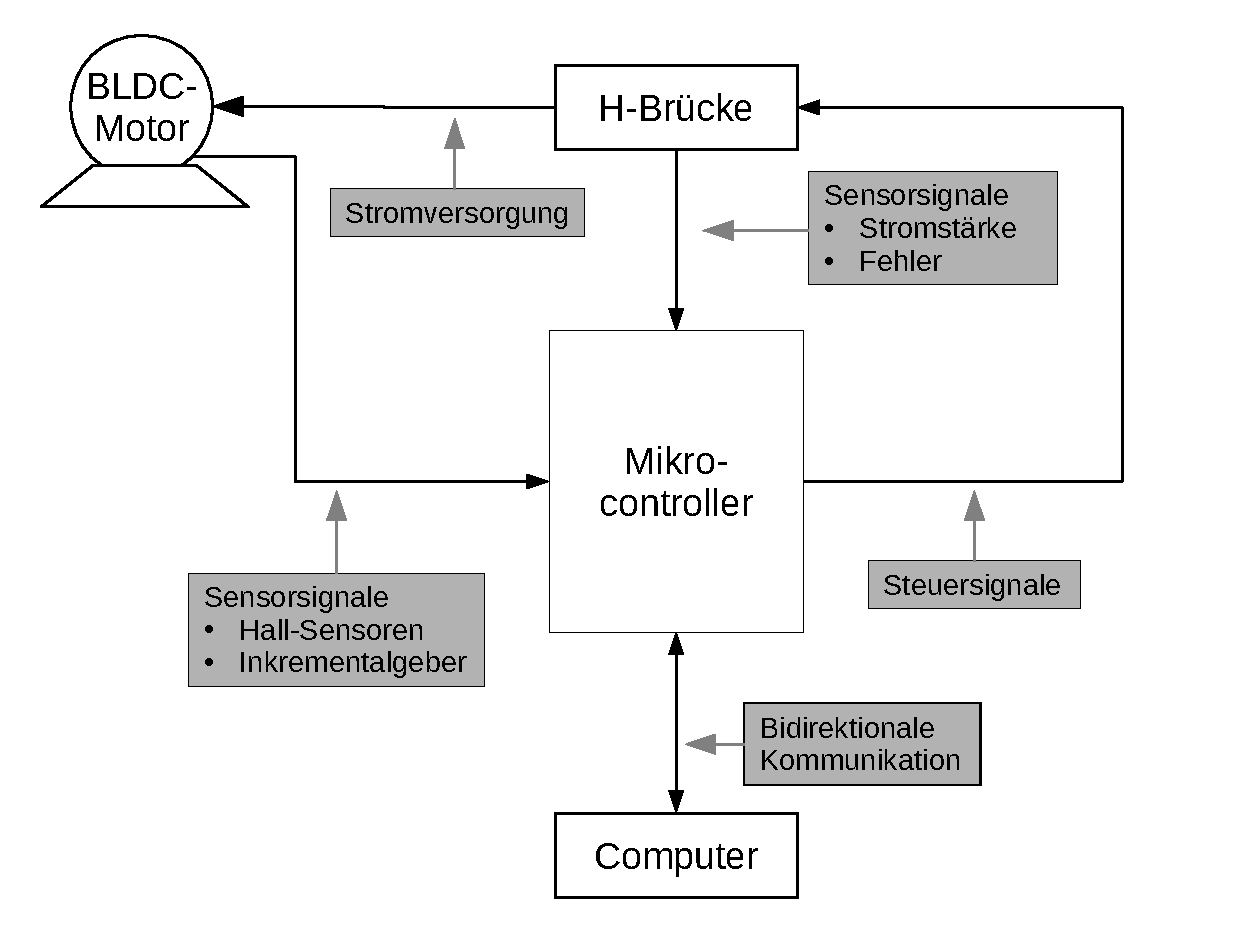
\includegraphics[width=\textwidth-4cm]{hardware/graphics/Schema_Uebersicht.pdf}
	\caption{Schematische Übersicht der einzelnen Hardwarekomponenten}
	\quelle Selbst erstellte Grafik
	\label{fig:Schemata_Hardware_Gesamt}
\end{figure}
\chapterauthor{Andreas Kölbl}

\chapter{Arbeitspaket Motor}
Die Analyse, Implementierung, Test und Integration, sowie die Verkabelung der H-Brücke mit Unterst\"utzung von Herrn Brunner f\"ur Hardware-relevante Problemstellungen war Aufgabe von Herrn Kölbl. Die Drehzahl des Motors soll gesteuert werden können.

\section{Analysephase}
Aus der Projektspezifikation ergibt sich, dass sich der Motor in zwei Richtungen drehen soll. Auch soll die Drehzahl des Motors einstellbar sein.

\subsection{Verkabelung Motor}
\begin{figure}
    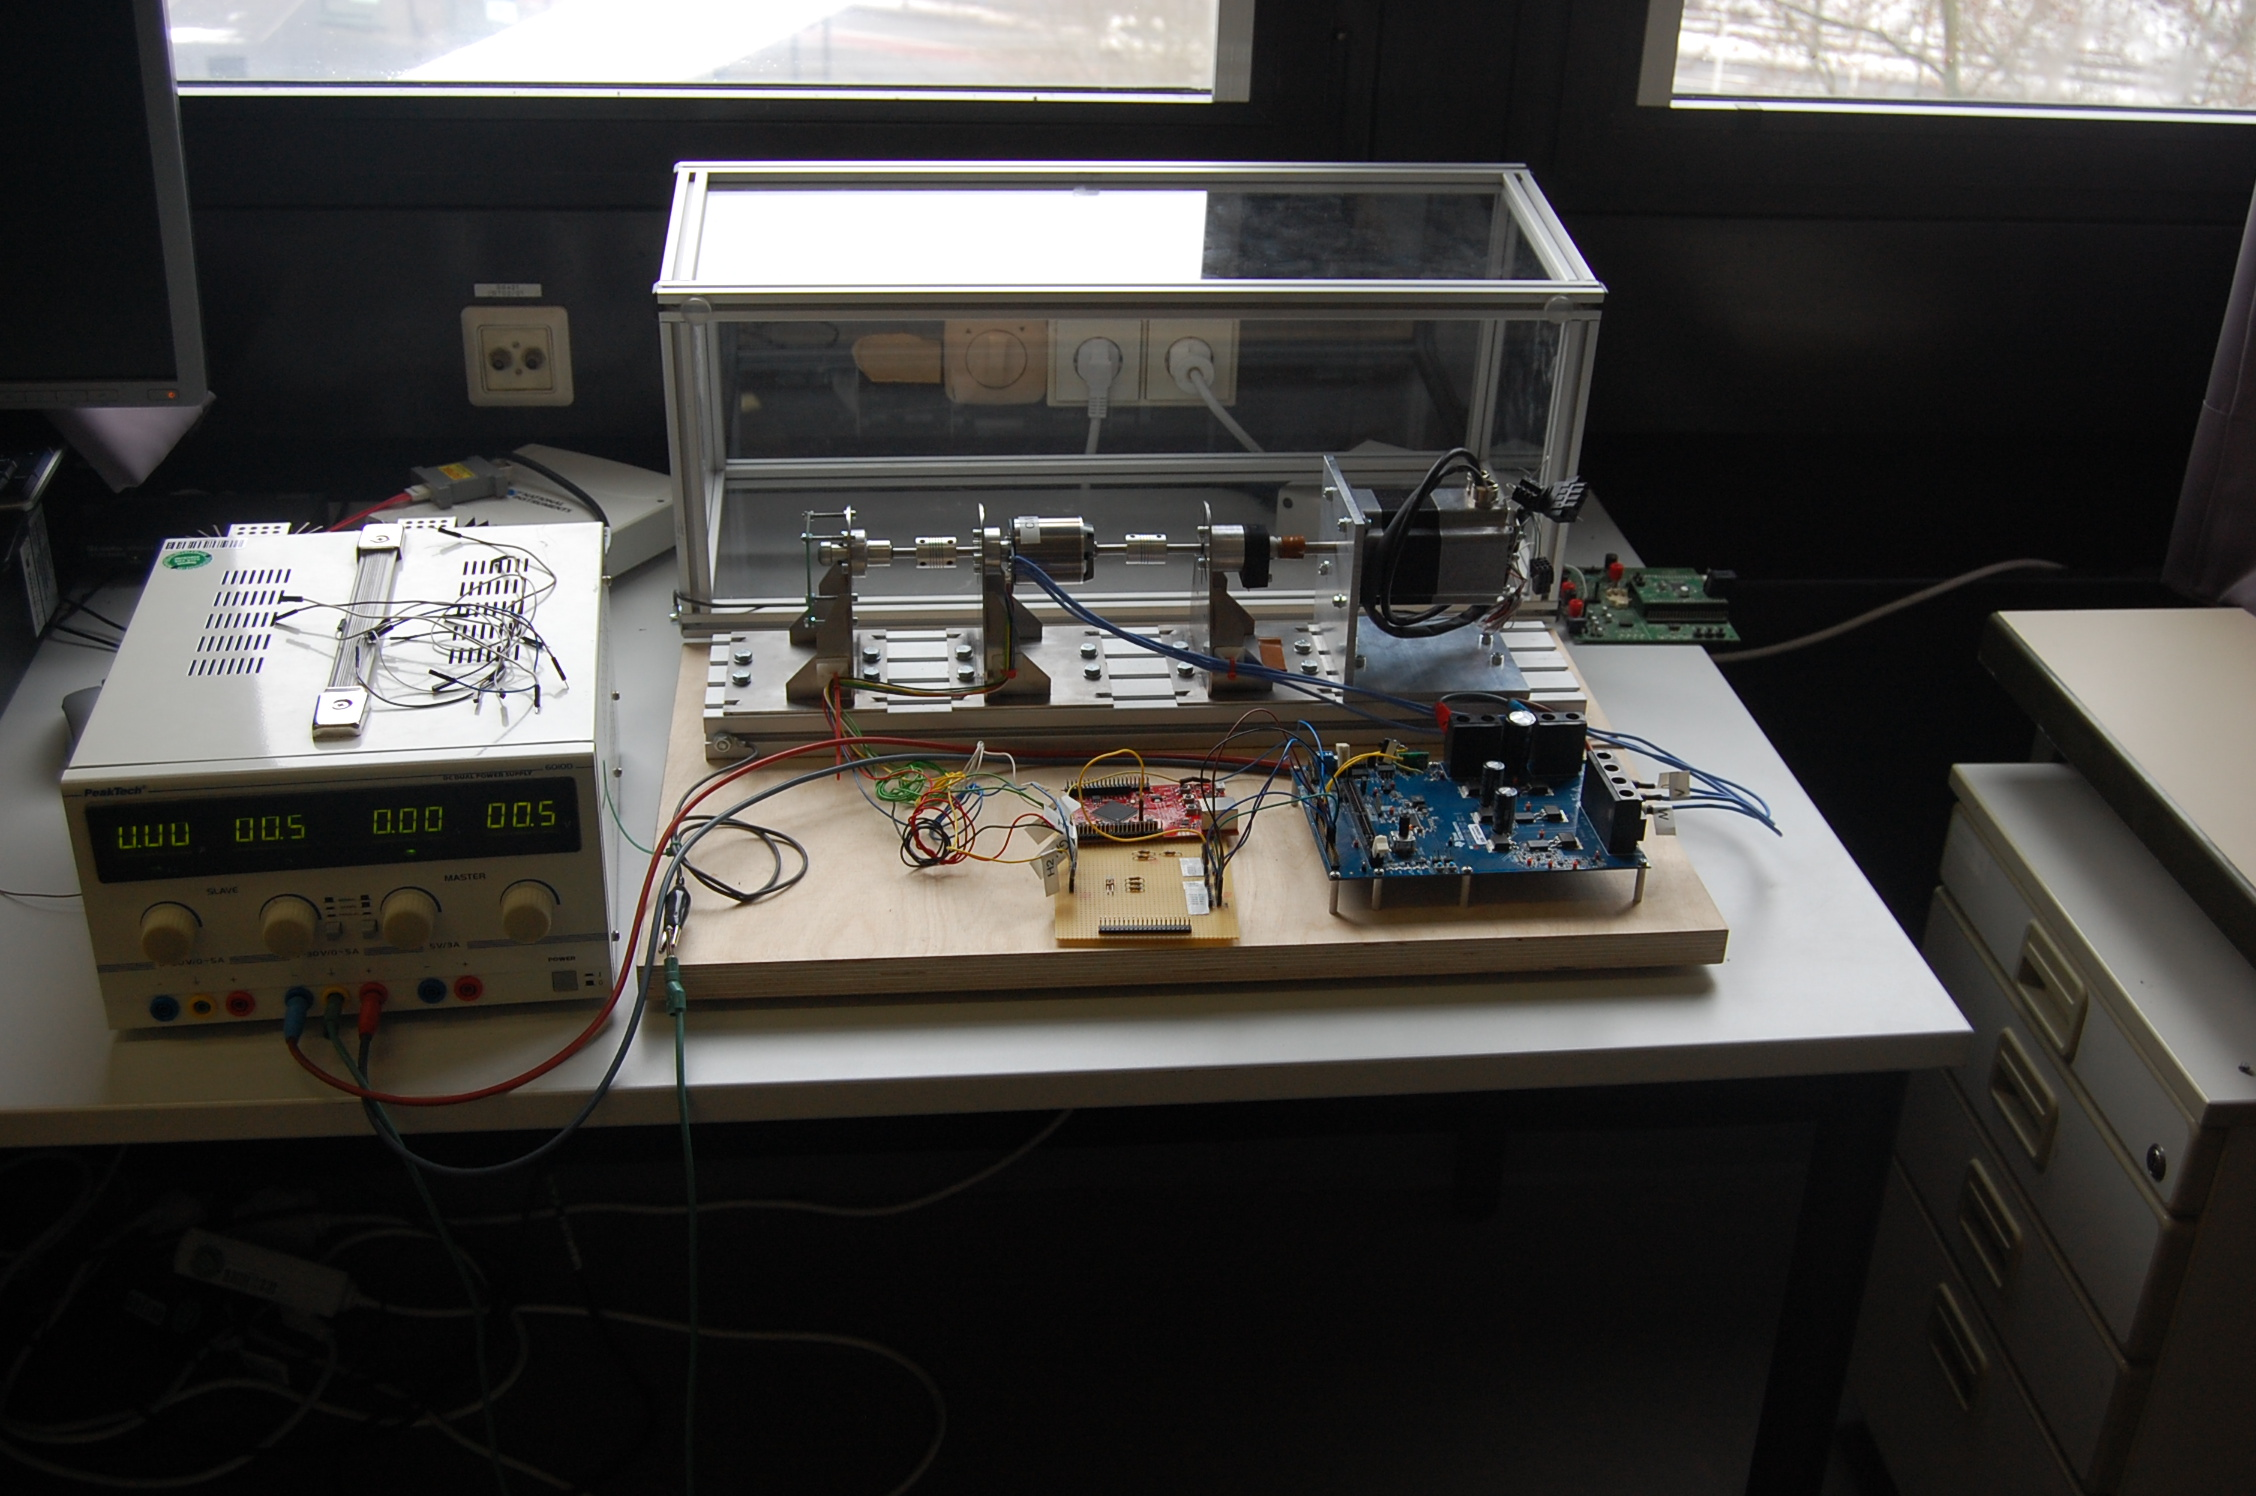
\includegraphics[width=\textwidth]{motor/MotorWiring.JPG}
    \caption{Verkabelung des Motors}
    \label{fig:MotorWiring}
\end{figure}

Die H-Brücke, die in Abbildung \ref{fig:MotorWiring} zu sehen ist, ist mit einem Netzteil (im ausgeschaltetem Zustand) und dem Motor verbunden. Es wäre auch ein Netzteil mit einer höheren Ausgangsspannung einsetzbar, da die H-Brücke bis zu 60V Gleichspannung betrieben werden kann. Das Erdungskabel zum Netzteil ist mit dem Motor verbunden. \\
Die H-Brücke ist außerdem noch mit der Adapterplatine gemäß dem Schaltplan verbunden. In dem Ausschnitt \ref{fig:TIWiring} ist der PIN-Header "External Control" zu sehen, der zur manuellen Kommutierung benutzt wird. Dabei sind die drei Phasen U, V und W mit deren jeweiligen High- und Low-Anschluss als PWM\_AH, PWM\_AL, PWM\_BH, PWM\_BL, PWM\_CH und PWM\_CL beschrieben. Diese sind mit dem Mikrocontroller zu verbinden. Dabei ist darauf zu achten, dass die jeweiligen Pins auf dem Controller für die Capture-Compare Units verwendet werden können \cite{InfineonTechnologies2016}.
\begin{figure}
    \includegraphics[width=0.66\textwidth]{motor/TI_Wiring.png}
    \caption{H-Brücke 40 Pin-Header}
    \quelle \cite{Instruments2014}
    \label{fig:TIWiring}
\end{figure}
Der Motor muss mit den Stromausgängen U, V und W verbunden werden. Die Kabel wurden für diesen Zweck beschriftet. \\

\subsection{BLDC-Motor}
Den Brushless DC-Motor zu verwenden bringt Vor- und Nachteile mit sich.

Der allgemeine Vorteil von Bürstenlosen Motoren liegt darin, dass es keine Verschleißteile gibt.
Hingegen müssen bei klassischen Gleichstrommotoren mit Bürsten diese ersetzt werden sobald sie verbraucht oder zerstört sind. Im Idealfall werden auch keine störenden Induktionsspannungen durch die Stromwendung erzeugt \cite{Babiel2014}. Der bürstenlose Motor läuft sehr leise und lässt sich sehr genau von ganz langsam (nicht alle) bis ganz schnell elektronisch regeln. Dazu hat er erheblich mehr Kraft bei gleichen Abmessungen oder einen geringeren Stromverbrauch mit weniger Verlustleistung. \\
Der Nachteil des BLDC-Motors ist, dass der Motor nicht stehen bleibt, wenn die Spannung weg ist. Er muss gezielt abgebremst und gestoppt werden.
Durch den deutlich höheren Preis sollten diese bürstenlosen DC Motoren nur in anspruchsvollen Geräten eingesetzt werden.
Die Auswahlkriterien für die bürstenlosen Gleichstromservomotoren sind meist "extrem präzise stufenlose Geschwindigkeit" bei sich stetig ändernder Last im geschlossenen Regelkreis mit Prozessorsteuerung.

\subsection{TI InstaSPIN}
Die von Texas Instruments gelieferte H-Brücke bietet zusätzlich zum manuellen Ansteuern eines Motors noch die Möglichkeit, diesen über das Programm InstaSPIN anzusteuern. Hierfür ist eine lizensierte Steuerkarte enthalten, die mit einer Testlizenz von 30 Tagen geliefert wurde. Eine Ansteuerung über ein virtualisiertes Windows-Betriebssystem war nicht möglich, da Linux als Betriebssystem nicht unterstützt wird. Dieses Programm führt eine Ansteuerung des Motors ohne Hall-Sensoren durch. Hierbei wird lediglich der Spannungsabfall am Stromausgang durch einen ADC-Converter gemessen und den Messwerten entsprechend kommutiert. Über den Drehregler in Abbildung \ref{fig:InstaSPIN} lässt sich die Drehzahl des Motors beeinflussen.
\begin{figure}
    \includegraphics[width=\textwidth]{motor/InstaSPIN}
    \caption{Texas Instruments InstaSPIN}
    \quelle \cite{Instruments2011}
    \label{fig:InstaSPIN}
\end{figure}
\section{Implementierung}
\subsection{POSIF}
\subsubsection{Zweck von POSIF}
Da Software als solches in der Erstellung und Pflege teurer wird und Hardwarekosten stetig sinken, ist ein Trend erkennbar, Software direkt als Hardware zu implementieren. Das Ergebnis sind bessere Schaltgeschwindigkeiten und weniger Kosten durch Programmierung und Wartung von Software. So erreicht man durch die besseren Schaltgeschwindigkeiten neue Rekorde, wie bspw. den \emph{Rubik's Cube} zu lösen \cite{POSIF2016}.

\subsubsection{Zuweisung im Multi-Channel Mode}
In Abbildung \ref{fig:interconnects} wird die interne Verschaltung des POSIF-Interfaces mit den jeweiligen Capture-Compare Units dargestellt. Die Capture-Compare Units geben das PWM-Signal auf deren jeweilig zugewiesenen Ausgängen aus, sobald ein neues \emph{Correct Hall Event} aufgetreten ist. Wie diese Zuweisung auszusehen hat, kann leider nur durch das lesen vieler Dokumente die auf der Website von Infineon bei den Chips der Serie XMC1000/XMC4000 erahnt werden. Letztlich gibt der Code vom XMC44xx-Chip von Infineon ein vorbildliches Beispiel, wie das POSIF-Interface zu implementieren ist. Es ist notwendig, die Variablen, die in Abbildung \ref{fig:interconnects} dargestellt sind, den entsprechenden Ausgängen zuzuweisen.  Leider wurde dieses Beispiel eines anderen Chips erst in einer sehr späten Projektphase entdeckt. Deswegen ist im Beispielcode das POSIF-Interface lediglich dazu da, Hall-Events weiterzuleiten. Je nach Hall-Event werden die Ausgänge zum Schalten der Motoren mit voller Leistung angetrieben.
\begin{figure}
    \includegraphics[width=\textwidth]{motor/interconnects}
    \caption{Verbindungen des Patterns zum Ausgang einer CCU Slice}
     \quelle {Infineon}
    \label{fig:interconnects}
\end{figure}

\section{Ausblick}
Der Code zur Steuerung und Regelung des Motors befindet sich momentan noch in den Anfängen. Bei der aktuellen Bearbeitungslage ist eine vollständige Fertigstellung nicht absehbar. \\
Basierend auf der Ideensammlung aus der Analysephase wäre eine mögliche Erweiterung dieses Arbeitspaketes die Portierung des Codes auf eine andere Hardwareplattform ohne POSIF-Interface. Das hätte eine Neuimplementierung der Steuerung zur Folge. \\
Der Beispielcode des POSIF-Interfaces, welches alle Features des POSIF-Interfaces nutzt wäre ein sinnvoller Ansatz, um eine Portierung vom XMC44xx-Chip zum XMC4800 vorzunehmen. Somit können alle Vorteile des POSIF-Interfaces ausgenutzt werden. \\
Die Verkabelung muss noch gesichert werden. Die H-Brücke soll außerdem während des Betriebs durch Eingriffe in die Elektronik geschützt werden, da an den auf der H-Brücke verbauten Kondensatoren sehr hohe Ströme auftreten können. 


\chapterauthor{Christian Brunner}

\chapter{Hardwaretest und Analyse}
\label{chap:Test_and_Analysis}
Dieses Kapitel beschäftigt sich mit Test und Analyse von Hardwarekomponenten, Aufbauten und elektrischen Signalen.
Es werden keinerlei Softwaretests im klassischen Sinn behandelt.
Der Fokus liegt dabei zu überprüfen ob und wie die einzelnen Komponenten Funktionieren bzw. welche Fehler auftreten bzw. auftreten können.

\section{BLDC Motor mit Fremderregung}
\label{sec:BLDC_mit_Fremderregung}
Zu Beginn des Projektes erhielten wir den Motor.
Da zu diesem Zeitpunkt noch keine Regelung bzw. Steuerung zur Verfügung stand stellte sich die Frage,
welches Signal der Motor benötigen würde.
Da ein Motor auch als Generator betrieben werden kann wurde, in Absprache mit Herrn Prof. Dr. Roth, mit wenigen Widerständen und einem Oszilloskop eine Messschaltung aufgebaut.\\


In Abbildung \ref{fig:BLDC_Fremderregung} ist der elektrische Aufbau zu sehen.
Auf der linken Seite bilden die drei Spulen (U, V und W) den Motor ab.
Rechts daneben befinden sich drei Messwiderstände.
Die Messsonden eines 2-Kanal-Oszilloskops wurde an die Leitungen U und V angeschlossen.
Anschlussleitung W diente als Bezugsmasse für die Messung.
Die Widerstandswerte, in der Abbildung mit 1 Kilo-Ohm angegeben, sind nur beispielhaft da diese mehrfach ausgetauscht wurden.
Die Messreihe umfasste dabei vier Messungen mit wechselnden Widerständen und geänderter Drehrichtung.


\begin{figure}[htbp]
	\centering
	\includegraphics[width=8cm]{tests/graphics/Messchaltung_Fremderregung}
	\caption[Aufbau Spannungsmessung BLDC Motor]{Messaufbau zur Messung der \\generierten Spannung am BLDC Motor}
	\label{fig:BLDC_Fremderregung}
\end{figure}


Durch das erzeugen einer Drehbewegung, mittels einer an die Motorwelle angebrachten Bohrmaschine, wurde in den Spulen eine Spannung erzeugt.
In Abbildung \ref{fig:Spannungsmessung_BLDC_Motor} ist eine dieser Messungen dargestellt.
Im oberen Bereich ist der Anlauf gut zu erkennen.
Die Spannung an den Spulen U und V sind ca. 120 $^\circ$ zueinander verschoben.\\


Ebenso wurden die drei Hall-Sensoren des Motors und das Indexsignal eines Drehgebers, welcher an der Motorwelle befestigt ist, aufgezeichnet.
Weiterhin ist in der Abbildung zu sehen, dass die Flankenwechsel der Hall-Sensoren verschoben sind.
Es gibt dabei ein Muster von sechs Zuständen, welche die Hall-Sensoren bilden können.
Aus der Überlegung drei Signale, die jeweils zwei unterschiedliche Zustände annehmen könnte es den Anschein haben, dass es acht ($2^3$) Zustände sein sollten.
Dem ist jedoch nicht so. 
Es gibt keinen Zustand, bei dem alle Signalleitungen HIGH bzw. LOW sind. Dadurch fallen diese weg.
Im Detail ist zu erkennen, dass es 42 Flankenwechsel für eine Umdrehung notwendig sind.

\begin{figure}[htbp]
	\centering
	\includegraphics[width=\textwidth-2cm]{tests/graphics/Spannungssignal_Messung}
	\caption{Spannungsmessung BLDC-Motor}
	\label{fig:Spannungsmessung_BLDC_Motor}
\end{figure}


Doch jede Messung ist nur so gut wie Ihr Messaufbau.
Dies musste im auch bei diesem Aufbau festgestellt werden.
Für die Erzeugung der Drehbewegung wurde, wie eingangs erwähnt, eine Bohrmaschine verwendet.
Dabei handelt es sich um ein Gerät mit Anschlussleitung.\\


Abbildung \ref{fig:Fehlerbehaftete_Spannungsmessung_BLDC_Motor} zeigt das Messergebnis, welches mit der Messschaltung aus Abbildung \ref{fig:BLDC_Fremderregung} gemessen wurde.
Im Vergleich zu \ref{fig:Spannungsmessung_BLDC_Motor} zeigt dieses Bild Spannungsspitzen und Verzerrungen.
Die Störungen aus dem Analogsignal wurden durch Einstreuung auch auf die digitalen Signale der Hall-Sensoren übertragen.
Zu erkennen sind diese durch die vielen kleinen Spitzen.
Zuerst konnte der Fehler nicht gefunden werden.
Es wurde der Messaufbau neu erstellt, neue bzw. andere Messleitungen und sogar ein anderes Oszilloskop verwendet.
All diese Maßnahmen halfen jedoch nicht den Fehler zu beseitigen.
Es stellte sich heraus, dass die Anschlussleitung der Bohrmaschine bei diesen Messungen direkt über den Messleitungen verlief.
Dabei wurden Störungen, die durch den Gleichstrommotor in der Bohrmaschine entstanden sind, auf die Messleitungen übertragen.


\begin{figure}[htbp]
	\centering
	\includegraphics[width=\textwidth-2cm]{tests/graphics/Fehlerhaftes_Spannungssignal}
	\caption{Fehlerbehaftete Spannungsmessung BLDC-Motor}
	\label{fig:Fehlerbehaftete_Spannungsmessung_BLDC_Motor}
\end{figure}


\section{Hall-Sensorsignale in Verbindung mit dem XMC 4700 Relax Kit 5V}
Wie bereits im Abschnitt Hardware angedeutet hat es während des Projektverlaufs Probleme mit der Auswertung von digitalen Signalen in Verbindung mit dem XMC 4700 Relax Kit 5V gegeben.

Im Abschnitt \ref{sec:BLDC_mit_Fremderregung} sind in einigen Abbildungen die Signale der Hall-Sensor zu erkennen.
Diese wurden nur mit einem Oszilloskop aufgezeichnet.
Zur besseren Darstellung soll Abbildung \ref{fig:Hall_Sensor_OK} dienen.
Dort sind die verschiedenen Flankenwechsel gut zu erkennen.
Das Signal nimmt definierte Werte an und schwingt nicht.


\begin{figure}[htbp]
	\centering
	\includegraphics[width=\textwidth-4cm]{tests/graphics/hall_ok}
	\caption[Sensorsignal Hall-Sensor]{Sensorsignal eines Hall-Sensors}
	\label{fig:Hall_Sensor_OK}
\end{figure}

Dieses Signal veränderte sich jedoch als die Hall-Sensoren mit dem XMC 4700 Relax Kit 5V verbunden wurden.
Bild \ref{fig:Hall_Sensor_Fehlerhaft} zeigt das gemessenen Signal.
Gut zu sehen ist, dass es die Pegel nur bei LOW (0 Volt) einen definierten Wert annehmen.
Bei einem Wechsel auf HIGH (5 Volt) begann das Signal zu schwingen.
Nach mehreren Versuchen, dass Signal mit Kondensatoren zu stützen geriet der auf dem Relax Kit verbaute Pegelwandler in Verdacht.

Als Folge wurde das XMC 4700 Relax Kit 5V gegen ein XMC 4800 Relax EtherCat Kit ausgetauscht.
Dieses Board besitzt keine Pegelwandler.
Nach dem Austausch verschwand das Schwingen auf den Signalleitungen.

Der Hersteller der Pegelwandler, Texas Instruments, verweist mehrfach im Datenblatt des Pegelwandlers darauf die Signalleitungen so kurz wie möglich zu halten.
Auch auf den verschiedenen Supportseiten des Herstellers ist dieses Phänomen häufiger beschrieben.
Testweise wurden die Anschlussleitungen zwischen Hall-Sensoren und XMC 4700 Relax Kit 5V stark verkürzt.
Dadurch konnte das Schwingen eliminiert werden.

\begin{figure}[htbp]
	\centering
	\includegraphics[width=\textwidth-4cm]{tests/graphics/hall_jitter_4700}
	\caption[Fehlerhaftes Sensorsignal eines Hall-Sensors]{Sensorsignal eines Hall-Sensors mit Störungen}
	\label{fig:Hall_Sensor_Fehlerhaft}
\end{figure}


\section{Steuersignale Relax Kit / H-Brücke}
Zur 



\section{Ansteuerungssignale Texas Instrument Evaluation Kit}

\section{Steuerungssignale }

\chapterauthor{ }
\listoffigures
\listoftables
\appendix
\chapterauthor{Michael Schleinkofer}
\chapter{Codeausschnitt aus der C\#-Bibliothek mit ComPort-Settings}
\label{ComAPP:ComPortSettings}
\begin{lstlisting}
private void port_Init()
{
  try
  {
    _uart.BaudRate = 9600;
    _uart.DataBits = 8;
    _uart.StopBits = StopBits.One;
    _uart.Handshake = Handshake.None;
    _uart.Parity = Parity.Even;
    _uart.DtrEnable = false;
    _uart.RtsEnable = false;
    _uart.DataReceived += uart_DataReceived;
    _uart.ReceivedBytesThreshold = 10;
    _uart.Open();
    _isInit = true;
  }
  catch(Exception e)
  {
    throw new SystemException("Uart init failed! Message: " + e.Message);
  }
}
\end{lstlisting}
\chapter{Codeausschnitt aus der C\#-Bibliothek zum Senden der Bytes}
\label{ComAPP:SendWait}
\begin{lstlisting}
  buf = Frameparser.EncapsuleFrame(buf);
  try
  {
    // ReSharper disable once UnusedVariable
    foreach (var elem in buf)
    {
      _uart.Write(buf, i, 1);
      i++;
      System.Threading.Thread.Sleep(30);
    }
    return true;
  }
  catch (Exception e)
  {
    throw new SystemException("Could not send Params! Error: " + e.Message);
  }
\end{lstlisting}

\chapter{Codeausschnitt aus der C\#-Bibliothek mit dem SoF-Automaten}
\label{ComAPP:SoFMachine}
\begin{lstlisting}
//Start of Frame checker
var state = 0; //state 0: no sof; state 1: 0x55 detected; state 2: 0x55 and 0xD5 detected
do{
  spL.Read(SofDel, 0, 1);
  if (state == 0 && SofDel[0] == 0x55)
  {
    state = 1;
    continue;
  }
  if(state == 1 && SofDel[0] == 0x55)
  {
    state = 1;
    continue;
  }
  if (state == 1 && SofDel[0] == 0xD5)
  {
    state = 2;
    continue;
  }
  if (SofDel[0] != 0x55 || SofDel[0] != 0xD5)
  {
    state = 0;
    continue;
  }
}while(state != 2);
state = 0;
//End of Frame Checker
\end{lstlisting}

\chapterauthor{ }
\chapterauthor{Michael Schleinkofer}
\chapter{Stundenzettel Michael Schleinkofer}
\begin{minipage}{0.5\textwidth}
    \begin{tabular}{llr}
       Datum& Tätigkeit&Stunden\\
       05.10.16&Anforderungsanalyse&3 \\
       07.10.16&Anforderungsanalyse&2 \\
       08.10.16&Anforderungsanalyse&5 \\
       11.10.16&Schnittstellen definieren&3 \\
       12.10.16&Schnittstellen definieren&3 \\
       14.10.16&Architekturentwurf&2 \\
       15.10.16&Architekturentwurf&5 \\
       18.10.16&Komponentenentwurf&3 \\
       19.10.16&Komponentenentwurf&3 \\
       21.10.16&Implementierung&3 \\
       22.10.16&Implementierung&5 \\
       25.10.16&Implementierung&3 \\
       26.10.16&Implementierung&3 \\
       31.10.16&Implementierung&5 \\
       02.11.16&Implementierung&3 \\
       04.11.16&Implementierung&2 \\
       05.11.16&Implementierung&5 \\
       08.11.16&Implementierung&3 \\
       09.11.16&Implementierung&3 \\
       11.11.16&Implementierung&1 \\
       12.11.16&Implementierung&4 \\
       15.11.16&Implementierung&3 \\
       16.11.16&Implementierung&3 \\
       18.11.16&Implementierung&2 \\
       19.11.16&Implementierung&4 \\
       22.11.16&Modultest&3 \\
       23.11.16&Modultest&3 \\
       25.11.16&Modultest&2 \\
       26.11.16&Modultest&4 \\
       29.11.16&Modultest&3 \\
       30.11.16&Modultest&3 \\
    \end{tabular}
\end{minipage}
\begin{minipage}{0.5\textwidth}
    \begin{tabular}{llr}
       Datum& Tätigkeit&Stunden\\
       02.12.16&Modultest&2 \\
       03.12.16&Modultest&4 \\
       06.12.16&Integration&3 \\
       07.12.16&Integration&3 \\
       09.12.16&Integration&1 \\
       10.12.16&Integration&4 \\
       13.12.16&Integration&3 \\
       14.12.16&Integration&3 \\
       16.12.16&Integration&1 \\
       17.12.16&Integration&4 \\
       20.12.16&Integration&3 \\
       21.12.16&Integration&3 \\
       23.12.16&Vorbereitung Präsentation&1 \\
       26.12.16&Dokumentation&6 \\
       27.12.16&Dokumentation&6 \\
       28.12.16&Dokumentation&6 \\
       10.01.17&Präsentation&1 \\
       &\textbf{Gesamt}&\textbf{153}
    \end{tabular}
\end{minipage}

\chapterauthor{ }
\chapter{Stundenzettel Ricardo Krause}
\begin{minipage}{0.5\textwidth}
    \begin{tabular}{llr}
       Datum& Tätigkeit&Stunden\\
       
       04.10.16&Anforderungsanalyse&5 \\
       05.10.16&Anforderungsanalyse&5 \\
       11.10.16&Schnittstellen definieren&3 \\
       12.10.16&Projektplan&3 \\
       12.10.16&Gruppenerfassungsbogen&2\\
       13.10.16&Git/Komunnikation &6\\
       18.10.16&Architekturentwurf&2 \\
       19.10.16&Architekturentwurf&5 \\
       25.10.16&Komponentenentwurf&5 \\
       26.10.16&Evaluation Controlls&5 \\
       02.11.16&Implementierung&6 \\
       03.11.16&Implementierung&6 \\
       08.11.16&Implementierung&6 \\
       09.11.16&Implementierung&6 \\
       11.11.16&Implementierung&3 \\
       15.11.16&Implementierung&6 \\
       16.11.16&Implementierung&6 \\



    \end{tabular}
\end{minipage}
\begin{minipage}{0.5\textwidth}
    \begin{tabular}{llr}
       Datum& Tätigkeit&Stunden\\
       19.11.16&Implementierung&3 \\
       22.11.16&Implementierung&6 \\
       23.11.16&Implementierung&6 \\
       26.11.16&Implementierung&6 \\
       29.11.16&Modultest&5 \\
       30.11.16&Modultest&5 \\
       06.12.16&Modultest&5 \\
       07.12.16&Integration&5 \\
       13.12.16&Integration&5 \\
       14.12.16&Integration&5 \\      
       20.12.16&Integration&5 \\
       21.12.16&Integration&5 \\
       23.12.16&Vorbereitung Präsentation&1 \\
       27.12.16&Dokumentation&6 \\
       28.12.16&Dokumentation&6 \\
       10.01.17&Präsentation&1 \\
       &\textbf{Gesamt}&\textbf{155}
    \end{tabular}
\end{minipage}
\chapterauthor{ }
\chapter{Stundenzettel Franz Welker}
\begin{minipage}{0.5\textwidth}
    \begin{tabular}{lp{4cm}r}
       Datum& Tätigkeit&Stunden\\
       
       04.10.16&Anforderungsanalyse&4 \\
       05.10.16&Anforderungsanalyse&3 \\
       
       11.10.16&Einarbeitung Simulink&6 \\
       12.10.16&Einarbeitung Simulink&4 \\
       12.10.16&Recherche nach \newline 
		        Simulink Modellen&2 \\
       
       18.10.16&Recherche nach \newline
		        Simulink Modellen&7 \\
       19.10.16&Evaluierung Simulink \newline
		        Modelle&6 \\
       19.10.16&Mithelfen bei anderen \newline
		        Gruppen&2 \\
       
       
       25.10.16&Recherche nach \newline
	            Simulink Modellen&2 \\
       25.10.16&Recherche Echtzeit \newline
		        Simulation&5 \\
       26.10.16&Recherche COM Ports&6 \\
       
       28.10.16&Simulink COM Blöcke einbauen&6\\
       02.11.16&Protobuf für Simulink&7 \\
       
       08.11.16&rotobuf für Simulink&2 \\
       09.11.16&Analyse Motoraufbau&7 \\
       
       15.11.16&Analyse Motoraufbau&4 \\
       15.11.16&Entwicklung neues \newline
		        Modell&3 \\
       16.11.16&Entwicklung neues \newline
		        Modell&7 \\



    \end{tabular}
\end{minipage}
\begin{minipage}{0.5\textwidth}
    \begin{tabular}{lp{4cm}r}
       Datum& Tätigkeit&Stunden\\
       
       22.11.16&Entwicklung neues \newline
		        Modell&6 \\
       23.11.16&Entwicklung neues \newline
		        Modell&2 \\
       23.11.16&Überarbeitung neues \newline
		        Modell&5 \\
       
       29.11.16&Überarbeitung neues \newline
		        Modell&3 \\
       29.11.16&Analyse neues Modell&3 \\
       30.11.16&Helfen in anderen \newline
			    Bereichen&6 \\
       
       06.12.16&Helfen in anderen \newline
		        Bereichen&6 \\
       07.12.16&Analyse neues Modell&3 \\
       07.12.16&Helfen in anderen \newline
		        Bereichen&5 \\
       
       13.12.16&Integration&5 \\
       14.12.16&Integration&5 \\ 
            
       20.12.16&Integration&5 \\
       
       22.12.16&Dokumentation&6 \\
       23.12.16&Dokumentation&6 \\
       25.12.16&Dokumentation&1 \\
       
       
       27.12.16&Dokumentation&3 \\
       03.01.17&Vorbereitung Präsentation&2 \\
       10.01.17&Präsentation&1 \\
       &\textbf{Gesamt}&\textbf{156}
    \end{tabular}
\end{minipage}
\chapterauthor{ }
\chapter{Stundenzettel Christian Brunner}
\begin{minipage}{0.5\textwidth}
    \begin{tabular}{lp{4.5cm}r}
		Datum		&	Tätigkeit				&Stunden	\\
					&							&			\\
		04.10.16	&	Anforderungsanalyse		&	5		\\
		05.10.16	&	Recherche				&	5		\\
		11.10.16	&	Recherche				&	5		\\
		12.10.16	&	Unterestützung \newline
						Teammitglieder			&	5		\\
		18.10.16	&	Unterestützung \newline
						Teammitglieder			&	5		\\
		19.10.16	&	Messungen und Analyse	&	5		\\
		25.10.16	&	Messungen und Analyse	&	5		\\
		26.10.16	&	Messungen und Analyse	&	5		\\
		02.11.16	&	Inbetriebnahme \newline
						Motorprüfstand			&	5		\\
		08.11.16	&	Inbetriebnahme \newline
						Motorprüfstand			&	5		\\
		09.11.16	&	Recherche H-Brücke		&	5		\\
		15.11.16	&	Test Fremderregung		&	5		\\
		16.11.16	&	Analyse Fremderregung	&	5		\\
		22.11.16	&	Diskussion Steuersignal	&	5		\\
		23.11.16	&	Unterstützung \newline
						Teammitglieder			&	5		\\
		

    \end{tabular}
\end{minipage}
\vline
\begin{minipage}{0.5\textwidth}
    \begin{tabular}{lp{4.5cm}r}
		Datum		&	Tätigkeit				&Stunden	\\
					&							&			\\
		29.11.16	&	Entwurf Adapterplatine	&	5		\\
		30.11.16	&	Aufbau Adapterplatine	&	5		\\
		06.12.16	&	Messungen und Analyse	&	5		\\
		07.12.16	&	Fehleranalyse \newline
						Hall-Sensoren			&	5		\\
		13.12.16	&	Recherche BLDC \newline
						Steuerungssignal		&	5		\\
		14.12.16	&	Recherche BLDC \newline
						Steuerungssignal		&	5		\\
		19.10.16	&	Messungen und Analyse	&	5		\\
		20.12.16	&	Messungen und Analyse	&	5		\\
		21.12.16	&	Anfertigung Präsentation	&	5	\\
		10.01.17	&	Präsentation	&	5	\\
		11.01.17	&	Dokumentation	&	5	\\
		17.01.17	&	Dokumentation	&	5	\\
		18.01.17	&	Dokumentation	&	5	\\
		11.01.17	&	Dokumentation	&	5	\\
		15.01.17	&	Dokumentation	&	5	\\
		16.01.17	&	Dokumentation	&	5	\\
			        &	\textbf{Gesamt}	&	\textbf{155}
    \end{tabular}
\end{minipage}
\chapter{Stundenzettel Andreas Kölbl}
\begin{minipage}{0.5\textwidth}
    \begin{tabular}{lp{4cm}r}
       Datum& Tätigkeit&Stunden\\
       
       04.10.16&Anforderungsanalyse&5 \\
       05.10.16&Anforderungsanalyse&5 \\
       
       11.10.16&Einarbeitung Microcontroller XMC4700&6 \\
       12.10.16&Einarbeitung H-Brücke&5 \\
       12.10.16&Einarbeitung Instaspin&5 \\
       
       18.10.16&Erstellen von Virtuellem Image fürs Projekt&7 \\
       19.10.16&Recherche POSIF&6 \\
       19.10.16&Recherche POSIF&2 \\
       
       
       25.10.16&Recherche Kommutierung&7 \\
       26.10.16&Recherche H-Brücke&6 \\
       
       28.10.16&Recherche POSIF&6\\
       02.11.16&Recherche POSIF&7 \\
       
       08.11.16&Recherche POSIF&5 \\
       09.11.16&Recherche POSIF&7 \\
       
       15.11.16&Analyse Motoraufbau&4 \\
       15.11.16&Analyse PWM&3 \\
       16.11.16&Recherche BLDC&7 \\


    \end{tabular}
\end{minipage}
\begin{minipage}{0.5\textwidth}
    \begin{tabular}{lp{4cm}r}
       Datum& Tätigkeit&Stunden\\
       
       22.11.16&Recherche BLDC&6 \\
       23.11.16&Implementierung in POSIF&2 \\
       
       29.11.16&Implementierung in POSIF&3 \\
       29.11.16&Implementierung in POSIF&3 \\
       30.11.16&Helfen in anderen \newline
			    Bereichen&6 \\
       
       06.12.16&Implementierung in POSIF&6 \\
       07.12.16&Implementierung in POSIF&3 \\
       07.12.16&Implementierung in POSIF&5 \\
       
       13.12.16&Integration&5 \\
       14.12.16&Integration&5 \\ 
            
       20.12.16&Integration&5 \\
       
       22.12.16&Dokumentation&6 \\
       23.12.16&Dokumentation&6 \\
       25.12.16&Dokumentation&1 \\
       
       
       27.12.16&Dokumentation&3 \\
       03.01.17&Vorbereitung Präsentation&2 \\
       10.01.17&Präsentation&1 \\
       &\textbf{Gesamt}&\textbf{156}
    \end{tabular}
\end{minipage}
\chapterauthor{ }
\bibliography{communication/comCite,hardware/bib_hardware,tests/bib_test,regulation/regCite,motor/bib_motor}
\end{document}
